\documentclass[acmsmall,screen,review,anonymous]{acmart}
\usepackage{bbm}
\usepackage{ebproof}
\usepackage{minted}
\usepackage{tikz-cd}
\usepackage{subcaption}

% Parameters {{{
\setcopyright{none}
\bibliographystyle{ACM-Reference-Format}
\citestyle{acmauthoryear}
\newtheorem{remark}{Remark}
%}}}

% Notations {{{
\newcommand{\kw}[1]{\ensuremath{ \mathsf{#1} }}
\newcommand{\ifr}[1]{\mathrel{[{#1}]}}
\newcommand{\que}{\circ}
\newcommand{\ans}{\bullet}
\newcommand{\vref}{\le_\kw{v}}
\newcommand{\mext}{\le_\kw{m}}
\newcommand{\refby}{\preceq}
\newcommand{\scref}{\sqsupseteq}
\newcommand{\screfd}{\sqsubseteq}
\newcommand{\unitset}{\mathds{1}}
\renewcommand{\preceq}{\preccurlyeq}
\newcommand{\intl}[1]{\underline{#1}}
%\newcommand{\caller}[1]{{\rtimes}#1}
%\newcommand{\callee}[1]{{\ltimes}#1}
\newcommand{\caller}[1]{\langle #1 ]}
\newcommand{\callee}[1]{[ #1 \rangle}
%}}}

% Names of things {{{
\newcommand{\ClightP}{\ensuremath{ \mathsf{ClightP} }}
\newcommand{\Clight}{\ensuremath{ \mathsf{Clight} }}
%}}}

% Custom symbols {{{
\makeatletter
\providecommand*{\cupdot}{%
  \mathbin{%
    \mathpalette\@cupdot{}%
  }%
}
\newcommand*{\@cupdot}[2]{%
  \ooalign{%
    $\m@th#1\cup$\cr
    \hidewidth$\m@th#1\cdot$\hidewidth
  }%
}
\makeatother
%}}}

%\title{Compositional Compiler Correctness with Encapsulated State}
\title{A Framework for Compositional Verification with
  Data Abstraction, Encapsulated State and Certified Compilation}

\begin{document}

\maketitle

\section*{New material} %{{{

\begin{definition}[Tensor product of simulation conventions] \label{def:sctens}
For the language interfaces $A$ and $B$,
the language interface $A \otimes B$ and $\mathbf{I}$
are defined as:
\[
  A \otimes B \::=\:
  \langle
    A^\que \times B^\que, \:
    A^\ans \times B^\ans
  \rangle
  \qquad
  \mathbf{I} := \langle \mathbbm{1}, \mathbbm{1} \rangle
\]
Moreover,
given $R_A : A^\sharp \Leftrightarrow A^\flat$
and $R_B : B^\sharp \Leftrightarrow B^\flat$,
we can define the simulation convention
$R_A \otimes R_B : A^\sharp \otimes B^\sharp
  \Leftrightarrow
  A^\flat \otimes B^\flat$
as follows:
\[
  R_A \otimes R_B \: := \:
    \big\langle
      W_A \times W_B, \:
      R_A^\que \times R_B^\que, \:
      R_A^\ans \times R_B^\ans
    \big\rangle
\]
\end{definition}

\begin{theorem}
$\mathbf{SC}$ under $\otimes$ is a symmetric monoidal category.
\end{theorem}

\subsection*{Protected explicit state}

The Kripke relation
$\Lambda_U \in \mathcal{R}_V(\mathbbm{1}, U)$
is defined by the rule:
\[
  \begin{prooftree}
    \infer0{u \Vdash * \ifr{\Lambda_U} u}
  \end{prooftree}
\]

\begin{definition}
For a set $U$,
the simulation convention $\caller{U} : I \Leftrightarrow U$
is defined as:
\[
  \caller{U} := \big\langle U,
      \Lambda_U,
      \Lambda_U
    \big\rangle
\]
\end{definition}

\begin{definition}
For a pointed set $U$,
the stateful simulation convention
$\callee{U} : I \leftrightarrow U$
is defined as
\[
  \callee U \: := \: \big\langle
      U, \,
      \Lambda_U, \,
      \Lambda_U, \,
      {=}_U, \,
      \top_U
    \big\rangle
\]
\end{definition}

\[
  \begin{tikzcd}[sep=large]
    \mathcal{C}\otimes\kw{mem}
      \ar[r, "\mathsf{ClightP}(M)"]
      \ar[d, equals] &
    \mathcal{C}\otimes\kw{mem}
      \ar[r, equals]
      \ar[d, leftrightarrow, "\mathcal{C} \otimes \kw{mem} \otimes \callee{p_0}"] &
    \mathcal{C}\otimes\kw{mem}
      \ar[dd, leftrightarrow, "\mathcal{C} \otimes \kw{mem} \otimes \callee{m_0}"]
    \\
    \mathcal{C} \otimes \kw{mem}
      \ar[r, "\mathsf{ClightP} \langle M \rangle"]
      \ar[d, leftrightarrow, "\mathsf{C} \otimes \kw{mem} \otimes \caller{\kw{mem}}"'] &
    \mathcal{C} \otimes \kw{mem} \otimes \kw{penv}
      \ar[d, leftrightarrow, "\mathcal{C} \otimes \kw{mem} \otimes R"]
    \\
    \mathcal{C} \otimes \kw{mem} \otimes \kw{mem}
      \ar[d, leftrightarrow, "\mathcal{C} \otimes {\bullet}"'] &
    \mathcal{C} \otimes \kw{mem} \otimes \kw{mem}
      \ar[d, leftrightarrow, "\mathcal{C} \otimes {\bullet}"]
      \ar[r, equals] &
    \mathcal{C} \otimes \kw{mem} \otimes \kw{mem}
      \ar[d, leftrightarrow, "\mathcal{C} \otimes {\bullet}"]
    \\
    \mathcal{C} \otimes \kw{mem}
      \ar[r, "\mathsf{Clight}(M)"] &
    \mathcal{C} \otimes \kw{mem}
      \ar[r, equals] &
    \mathcal{C} \otimes \kw{mem}
  \end{tikzcd}
\]

\[
  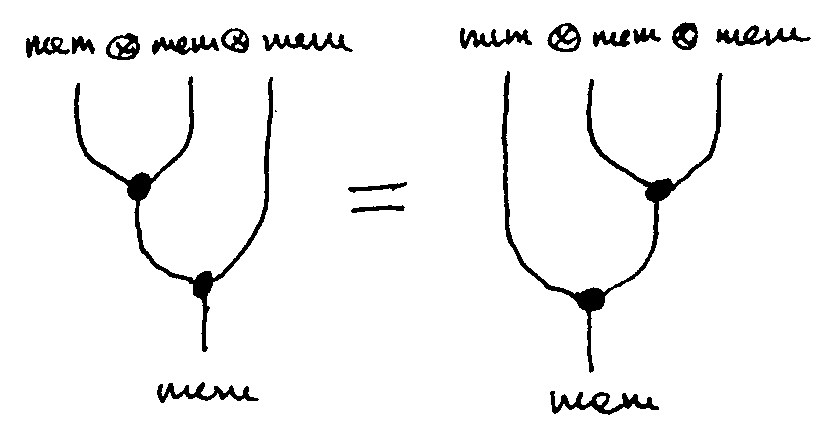
\includegraphics[scale=0.18]{draftfig/assoc}
\]

\[
  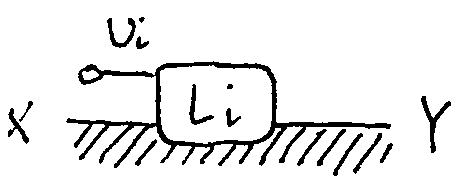
\includegraphics[scale=0.16]{draftfig/encap}
  \qquad\qquad
  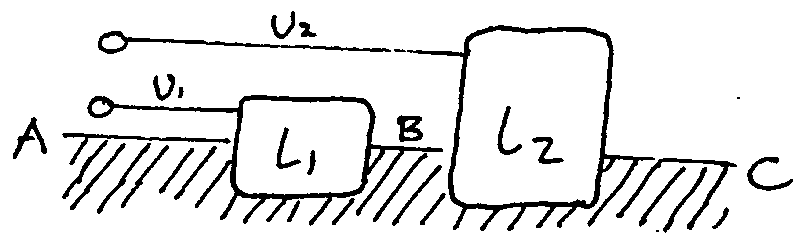
\includegraphics[scale=0.16]{draftfig/encap-comp}
\]

\[
  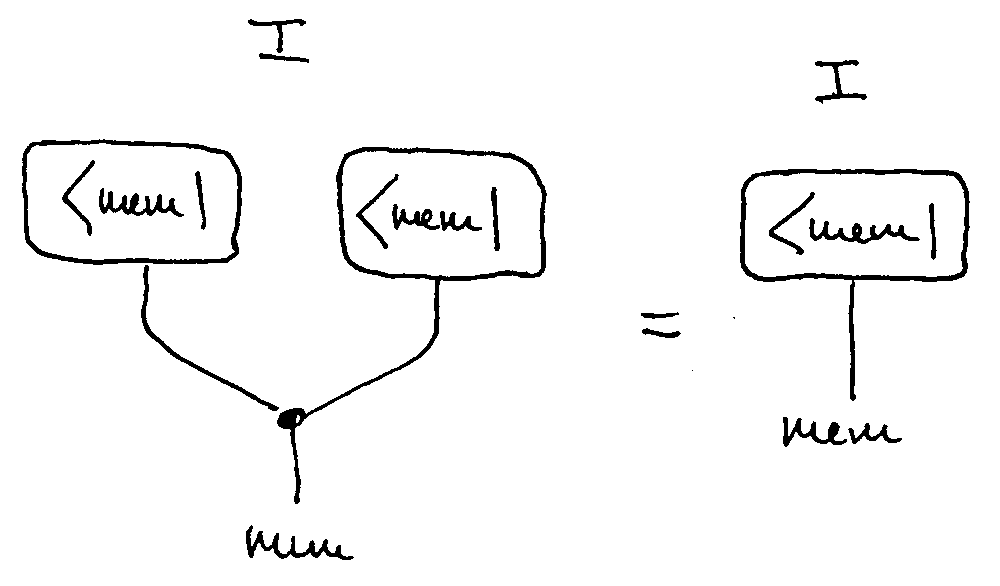
\includegraphics[scale=0.12]{draftfig/merge-caller}
  \qquad\qquad
  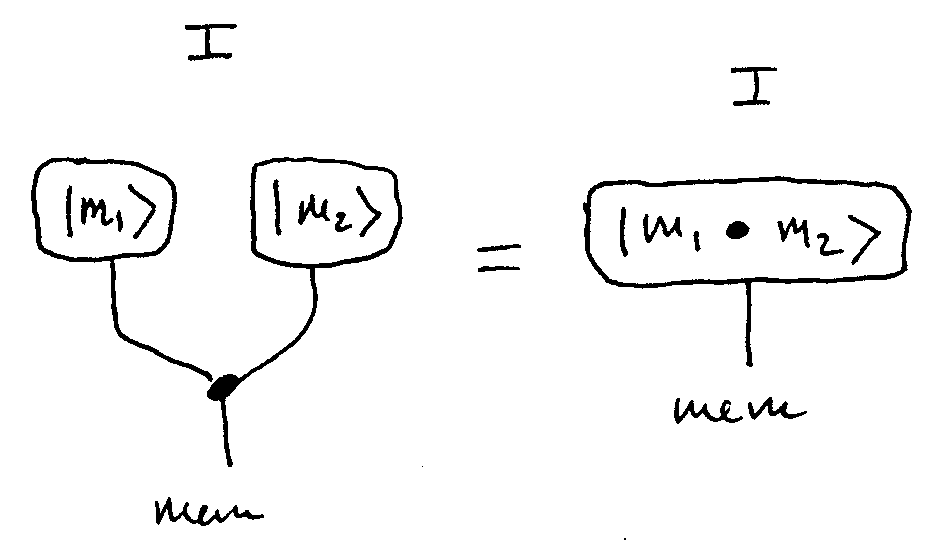
\includegraphics[scale=0.12]{draftfig/merge}
\]

%}}}

\section{Introduction} \label{sec:intro} %{{{

% Preamble {{{

Formal verification is the gold standard
for building reliable computer systems.
\emph{Certified} systems in particular
come with a formal specification,
and with a proof of correctness
which can easily be checked by a third party
\cite{shao10}.
Unfortunately, verifying large-scale, heterogeneous systems
remains out of reach of current techniques.
Addressing this challenge
will require the use of compositional methods,
making it easier to construct certified systems
from off-the-shelf certified components
\cite{deepspec}.

In principle,
compositional semantics
could play a key role in enabling this.
But in practice, simpler operational models
have proven more amenable
to carrying out actual verification projects.
This paper is concerned with bridging this gap.
%In particular,
%we examine the role of \emph{state encapsulation}
%in connecting low-level, operational models
%of software components on one hand,
%and more abstract and compositional models
%on the other hand.

%}}}

\subsection{Verification Frameworks} \label{sec:intro:bigpict} %{{{

Building large-scale certified systems
requires the ability
to model and specify those systems compositionally,
so that verification can be carried out
on components of a manageable size.
In addition,
the verification of large heterogeneous systems---%
for example,
computer systems involving combinations of
hardware, software and network components---%
will require models versatile enough
to account for the large variety of
operational paradigms and interfaces involved.

Devising models that are up to the task is challenging,
but existing research has laid much of the necessary groundwork.
Denotational semantics and category theory
excel at describing and manipulating compositional structures.
They tend to focus on the externally observable behavior of components,
abstracting away any internal details which are irrelevant
to the ways in which components interact and combine.
In principle,
they could be used to achieve
large-scale compositionality for certified components.
However,
category theory and denotational semantics
have not seen widespread adoption
for certified software engineering.

By necessity,
many certified software projects use
specialized semantic models,
chosen first and foremost
to make verification tractable
in the context of a particular
programming language or verification target.
Any compositional structures they provide
are likewise fine-tuned to their particular setting.
In this context,
mandating the use of any one model
%in order to achieve interoperability between
%certified system components
is unrealistic.
Instead,
researchers should attempt to establish
a hierarchy of semantic models
with varying degrees of generality.
Simple models could be used
in specific contexts in order to facilitate verification.
At the same time,
the resulting specifications and proofs
could be embedded into more flexible models
where they could interface
with other components.

With that said,
the high level of abstraction and generality of
existing compositional semantics
is not the only thing
standing in the way of their use for verification.
As a general rule,
work of this kind has focused on characterizing exactly
the space of behaviors which can be defined in a particular language.
By contrast,
verification often operates in much more open-ended settings.
The focus is the relationship between specifications and implementations,
involving both abstraction and program refinement.
A better understanding of how these concepts fit into
the paradigm of compositional semantics
is therefore another important task
to make the construction of
large-scale, heterogeneous, certified systems
tractable.

%In this paradigm,
%suitable high-level models would need to account
%for specifications, refinement and abstraction,
%which have not been a traditional focus
%for denotational semantics
%but which are the bread and butter of
%many verification frameworks.
%Conversely,
%compositional structures
%used in low-level models to facilitate verification
%should ideally be designed in such a way that
%they can be preserved when embedded into richer settings.
%This would allow compositional reasoning
%to cut across components of different kinds,
%even when they were originally verified
%using different low-level frameworks.

%In what follows,
%we use this lens
%to examine recent work on
%the certified compiler CompCert.

%We present a formal account
%of both horizontal and vertical compositionality
%as well as the \emph{certified abstraction layer}
%techniques used to verify
%the operating system kernel CertiKOS.
%We identify \emph{double categories}
%as an account of structures found in CompCertO,
%an extension of CompCert
%which provides a compositional semantic preservation theorem.
%We outline a high-level account
%of this semantic model
%and show how these high-level structures
%can be used to facilitate
%an implementation of certified abstraction layers
%within the framework provided by CompCertO.

%}}}

% xx where do interaction trees fit in the picture

\subsection{CompCert} %{{{

Work on
the certified C compiler CompCert \cite{compcert}
illustrates many challenging aspects of compositional verification.
CompCert is a C compiler written in the Coq proof assistant
which comes with a formal, mechanized proof of correctness:
the semantics of the source and target languages
are described as labeled transition systems,
and a simulation proof
shows that the behavior of the compiled program
refines the behavior of the source program.

%The original correctness theorem of
Originally,
CompCert
only modeled the compilation of whole programs.
To overcome this limitation,
researchers first attempted to make
the transition system model used by CompCert
more compositional,
and to update the compiler's semantic preservation property
to operate at the level of individual translation units
\cite{compcompcert}.
Because
this came at a high cost in terms of proof effort,
subsequent work on verified separate compilation
turned instead to the development of compositional
\emph{proof techniques}
within the context of a closed, whole-program semantics
(\S\ref{sec:related:compcert}).
%Another successful approach
%was explored by the work
However,
the recent work on CompCertO \cite{compcerto}
revisits compositional semantic preservation,
addressing its challenges
by incorporating data refinement
as a first-class citizen.
The flexibility
gained by this approach
makes it possible %---as in CompCertM---%
to reuse much of CompCert's existing
correctness proofs,
and to address any difficulties in composition
using external reasoning.

The semantic model of CompCertO
remains fairly specialized:
its goal is to minimize any changes needed to CompCert,
to eliminate any unnecessary complexity,
and to enable compositionality
to the exact extent required
for compositional semantic preservation to work.
%In particular,
%the model does not account for
%encapsulated state;
%it describes the behavior of individual function calls,
%independently of any prior history,
%and expect any persistent state
%to be passed by the environment at entry
%alongside the names and parameters of the function to be invoked.
%
Yet
the directness of the approach
%in terms of the programme outlined in \S\ref{sec:intro:bigpict},
%CompCertO's approach also opens up the possibility
opens the door to
a compositional embedding
of CompCertO's semantics and proofs
into richer models.
In fact,
we will show that CompCertO's model
already exhibits a surprisingly rich compositional structure,
and that once this structure has been brought to light,
it can be extended to account for encapsulated state
using fairly general constructions.

%We will show that CompCertO's model
%can be equipped with the structure of
%a \emph{double category}.
%Based on this view
%of CompCertO's open semantics,
%we can further extend the framework
%to support state encapsulation.
%Moreover,
%once they are brought to light,
%we can give an account of
%these compositional structures
%in terms of simpler and more abstract models,
%such as Reddy's
%coherence space model of objects
%\cite{objsem}.
%
%The main difficulty encountered in this work
%is the difference in data representation
%in the semantics of source and target programs.
%In CompCert's closed semantics,
%these differences play no role in
%the externally observable behavior of programs.
%Consequently,
%simulation proofs can capture these differences
%in the simulation relations they use.
%Simulation relations are existentially quantified
%within proofs,
%and can remain hidden in correctness statements.
%By contrast,
%in the context of compositional semantics,
%cross-component interactions which occur
%within a linked program become observable,
%and these internal details can no longer be ignored.

%}}}

\subsection{Certified abstraction layers} %{{{

The divide between abstract semantic models
and concrete verification projects
also exists in the context of \emph{certified abstraction layers},
a technique which
allows a complex program to be verified in steps,
and which was used in the construction of
the certified operating system kernel CertiKOS
\cite{popl15,ccal}.

Under this approach,
the verification begins first with the lowest-level layer of code,
which other parts of the program rely on.
Once verified,
this code can be given a high-level specification,
which hides the implementation details
and makes it possible to reason about client code
in terms of an abstract view
of the lower layer's state.
This abstract state
can be accessed only by calling into
the layer's interface,
realizing a form of state encapsulation
and data abstraction.

To implement this methodology,
CertiKOS uses a modified version of CompCert
called CompCertX,
which parameterizes the compiler's semantics and correctness proof
with a layer interface.
This requirement [is a problem but now we have a general-purpose CompCertO].

%This approach was 
%
%There are limitations to the way this approach
%was implemented for the verification of CertiKOS.
%This work reused the CompCert semantics,
%by augmenting its memory model
%with a layer-dependent \emph{abstract state} component,
%making it possible to connect the code verification
%with the compiler's correctness proof.
%However,
%this means that the formulation of certified abstraction layers
%used in this context
%was intimately tied to CompCert-specific constructs.

In addition,
while this approach allows code
to be verified in a piecemeal manner,
and allows reasoning at an appropriate level of abstraction
for each layer,
the method is not fully compositional
in the sense that it relies on \emph{closed} semantics.
The behavior of a given abstraction layer
can only be characterized
once a specification for the lower layer it builds on has been given,
reducing the flexibility of the framework.
This also forces verification to proceed
in a linear way,
so that when two parts of the code
are independent,
one must nonetheless be verified
as a client to a layer which includes the other.

To address these limitations,
more abstract models have been proposed
for certified abstraction layers
\cite{rbgs-cal,popl22},
inspired by game semantics and
coherence space models of objects \cite{objsem}.
These models have not been used
in the context of practical verification tasks,
but shed light on the underlying structures
involved in this methodology.

Based on our framework,
we propose a formulation of certified abstraction layers
which incorporates the best of both worlds:
on one hand,
like the original formulation,
it is based on CompCertO semantics
and seamlessly integrates
with the compiler's correctness theorem;
on the other hand,
like more recent work,
the categorical structures underlying its construction
are made explicit,
facilitating a more compositional approach
to certified abstraction layers.
To illustrate these capabilities,
we demonstrate the use of this framework
by verifying a simple example
found in prior work.

%}}}

\subsection{Contributions} %{{{

We extend the semantic model of CompCertO in several directions:
\begin{itemize}
\item
  In \S\ref{sec:base},
  we lay out the formal structure of
  our approach to refinement, abstraction and state.
  We extend the semantic model of CompCertO
  with a categorical composition operator
  ${\odot}_{A,B,C} : (B \twoheadrightarrow C) \times (A \twoheadrightarrow B)
    \rightarrow (A \twoheadrightarrow C)$.
  In conjunction with simulation conventions and their own compositional structure,
  this equips the model with the structure of a \emph{double category}.
  In addition,
  we make explicit CompCertO's approach to \emph{state}
  and introduce formal constructions
  for more flexible ``state plumbing''.
\item 
  In \S\ref{sec:encap},
  we derive a new model
  which permits \emph{state encapsulation}.
  Instead of managing state as an explicit part of component interfaces,
  we make it possible to \emph{hide}
  all or part of a component's persistent state.
  In this model,
  we identify components which differ in
  the details of their encapsulated state,
  but whose behavior upon successive activations
  appears identical to the environment.
  Abstracting the details of internal state in this way
  facilitates high-level reasoning.
\item
  To illustrate these capabilities,
  we introduce $\ClightP$ (\S\ref{sec:clightp}),
  a version of the $\Clight$ language
  featuring module-local private variables.
  In the semantics of a $\ClightP$ component,
  private variables are encapsulated.
  $\ClightP$ programs can be compiled to $\Clight$
  by transforming private variables into
  regular global variables.
  We show how the behavior of the $\ClightP$ program
  can be related to that of the corresponding $\Clight$ program,
  even though private variables become explicit state in the latter.
\item
  In \S\ref{sec:sep},
  we show how \emph{separation algebras} fit within our model.
  Specifically,
  a separation algebra on a set of states $K$
  allows a single global state of type $K$
  to be seen at a higher level of abstraction
  as two different fields ($K \times K$).
  This can be applied to the CompCert memory model
  to selectively encapsulate part of the memory
  as module-local state.
\item
  Finally,
  we use \emph{certified abstraction layers} \cite{popl15}
  as a case study to assess the capabilities of our model.
  In contrast with their original formulation,
  the flexibility of our model allows us
  to decouple to a large extent
  the formulation of layer interfaces
  from the details of CompCert programs
  used to implement them.
\end{itemize}

%}}}

% Old intro stuff
%
%% Preamble {{{
%
%Compilers are a critical component
%of modern computing environments.
%Therefore, ensuring their reliability
%is an important goal.
%To this end,
%certified compilers such as CompCert \cite{compcert}
%come with a formal semantics for source and target programs,
%and a proof of correctness which relates
%the behavior of compiled programs to that of their corresponding source.
%
%In this context,
%the quality of a compiler's correctness theorem
%may be judged in terms of its faithfulness
%to real-world use:
%are the source and target language semantics accurate?
%Does the correctness property relating them
%realistically model the way the compiler is used,
%and the target code executed?
%A high quality correctness theorem will provide stronger reliability guaranteed,
%and reduce the chance of bugs being introduced
%during program compilation.
%Empirical evaluation seems to confirm the benefits of this approach,
%at least in the case of CompCert \cite{csmith}.
%
%Moreover,
%certified compilers can also be important tools
%for \emph{building} other certified systems.
%Here,
%the compiler correctness proof itself
%will become a component within
%the correctness proof of a potentially larger
%and more heterogeneous system.
%This creates additional demands on
%the compiler's correctness theorem:
%is it convenient to interface with the rest of the proof,
%when the target code becomes part of a larger system?
%Can the compiler proof integrate into
%a compositional reasoning framework
%with a larger horizon than the program being compiled?
%
%%Can the compositional structures of the source language
%%be accounted for, and put in correspondence
%%with the compositional structures of the target language?
%%Finally,
%%can these compositional structures be subsumed within
%%a larger framework for compositional reasoning,
%%whose horizon goes beyond the boundary of
%%the target program?
%
%In this paper,
%we evaluate the capabilities of CompCertO \citep{compcerto}
%within this paradigm.
%CompCertO is
%a version of the certified compiler CompCert
%featuring compositional language semantics
%and a compositional correctness theorem.
%We show that with modest extensions,
%the semantic model used in CompCertO
%can support various forms of
%high-level, algebraically oriented compositional reasoning.
%The language semantics and correctness theorem of CompCertO
%can be reused as-is within this framework.
%
%%}}}
%
%\subsection{The CompCert Verified Compiler} %{{{
%
%The extensive body of research
%on the verified C compiler CompCert
%illustrates the different facets and roles
%certified compilers can take on.
%
%In its original form \citep{compcert},
%the correctness theorem of CompCert
%characterizes the compiler's use on complete, sequential C programs.
%Since then,
%efforts have been made to prove more realistic versions
%of the correctness theorem,
%covering use cases such as separate compilation \citep{sepcompcert},
%the compilation of
%code intended to run in a concurrent setting \citep{compcerttso},
%or stronger versions of correctness
%establishing for example
%guarantees on stack consumption of the target program \citep{qompcert}.
%
%Another line of work
%seeks to enable the use of CompCert's correctness theorem
%as an ingredient in
%other verification projects.
%Here,
%the ability to decompose programs and specifications
%is essential,
%so that components of manageable size can be verified in isolation.
%Compositional CompCert \cite{compcompcert} achieved this 
%by giving compositional semantics to the languages of CompCert,
%then expressing the correctness theorem at the level of individual components,
%but only at the expense of a significant increase in proof complexity.
%CompCertX \cite{popl15}, CompCertM \cite{compcertm} and CompCertO \cite{compcerto}
%
%[\ldots]
%
%%}}}
%
%\subsection{Large-scale verification} %{{{
%
%[While there are many verification frameworks
%which use CompCert in some capacity,
%none of them support encapsulated state.
%At most, permissions,
%but here the context still ``sees'' the memory,
%even though it must be shown to be insensitive to it.]
%
%%}}}

%}}}

\section{Overview of the Framework} %{{{

\subsection{Semantics in CompCertO} %{{{

% Language Interfaces {{{

The compositional semantics of CompCertO uses %revolves around
a notion of open transition system $L : A \twoheadrightarrow B$.
The type $A \twoheadrightarrow B$ involves
two \emph{language interfaces} $A$ and $B$,
which decribe how components interact.

\begin{definition} \label{def:li} %{{{
A \emph{language interface} $A = \langle A^\que, A^\ans \rangle$
is a set of questions $A^\que$ and a set of answers $A^\ans$.
\end{definition}
%}}}

Two important language interfaces
are involved in formulating the CompCertO correctness theorem.
The language interface $\mathcal{C}$
models interactions between C translation units.
The language interface $\mathcal{A}$
is used to describe the behavior of assembly-level components.

\begin{example}[The $\mathcal{C}$ language interface] \label{ex:langint} %{{{
When a C component is invoked,
the environment specifies a function to be called
and argument values.
When the function is done executing,
control switches back to the environment
and the component specifies a return value.
This can be described by the language interface $\mathcal{C}$,
defined as follows:
\begin{align*}
  \mathcal{C}^\que &:= \{ f(\vec{v}) \mid f \in \kw{ident}, \vec{v} \in \kw{val}^* \}
  \\
  \mathcal{C}^\ans &:= \kw{val}
\end{align*}
In addition,
C programs may access and alter the global memory state.
This means that the current memory state must be attached
to every function call,
and an updated state must be communicated back
alongside the return value.
To this end, CompCertO uses the following language interface:
\begin{align*}
  (\mathcal{C} \mathbin@ \kw{mem})^\que &:=
    \{ f(\vec{v})@m \mid f \in \kw{ident}, \vec{v} \in \kw{val}^*, m \in \kw{mem} \}
  \\
  (\mathcal{C} \mathbin@ \kw{mem})^\ans &:=
    \{ v@m' \mid v \in \kw{val}, m \in \kw{mem} \}
  \,.
\end{align*}
\end{example}
%}}}

%Language interfaces specify the information exchanged between
%a component and its environment
%when control switches between the two.
%Questions correspond to function invocations
%and answers correspond to the function returning.
%An execution of the component $L : A \twoheadrightarrow B$
%is initiated with a question $q \in B^\que$
%and terminates with a corresponding answer $r \in B^\ans$.
%At any point during the execution,
%$L$ may ask a question $m \in A^\que$ (an external call),
%in which case it is suspended until an answer $n \in A^\ans$
%resumes the execution.

%}}}

\begin{figure} % fig:overview:ts {{{
  \[
    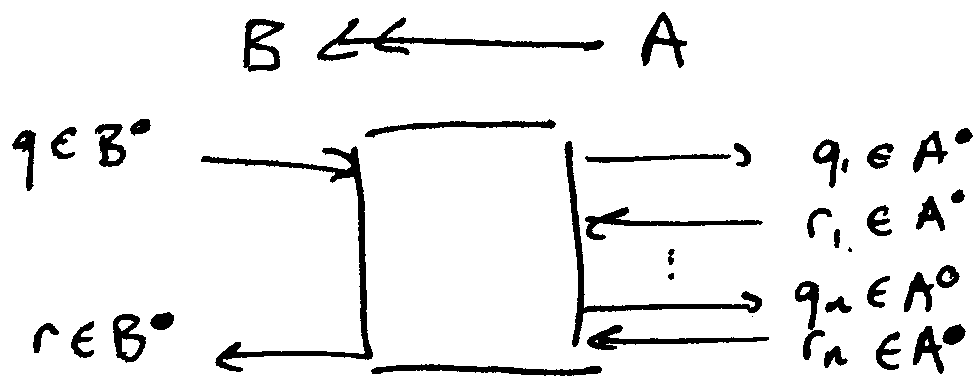
\includegraphics[scale=0.1]{draftfig/interaction}
    \qquad
    \vcenter{ \hbox{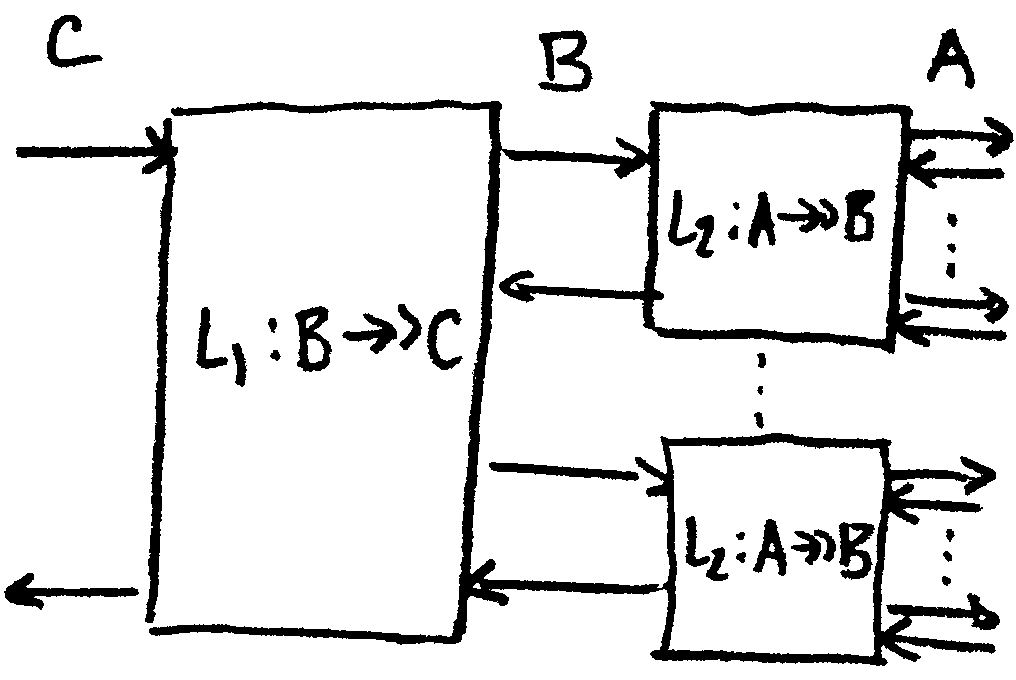
\includegraphics[scale=0.1]{draftfig/composition}} }
    \qquad
    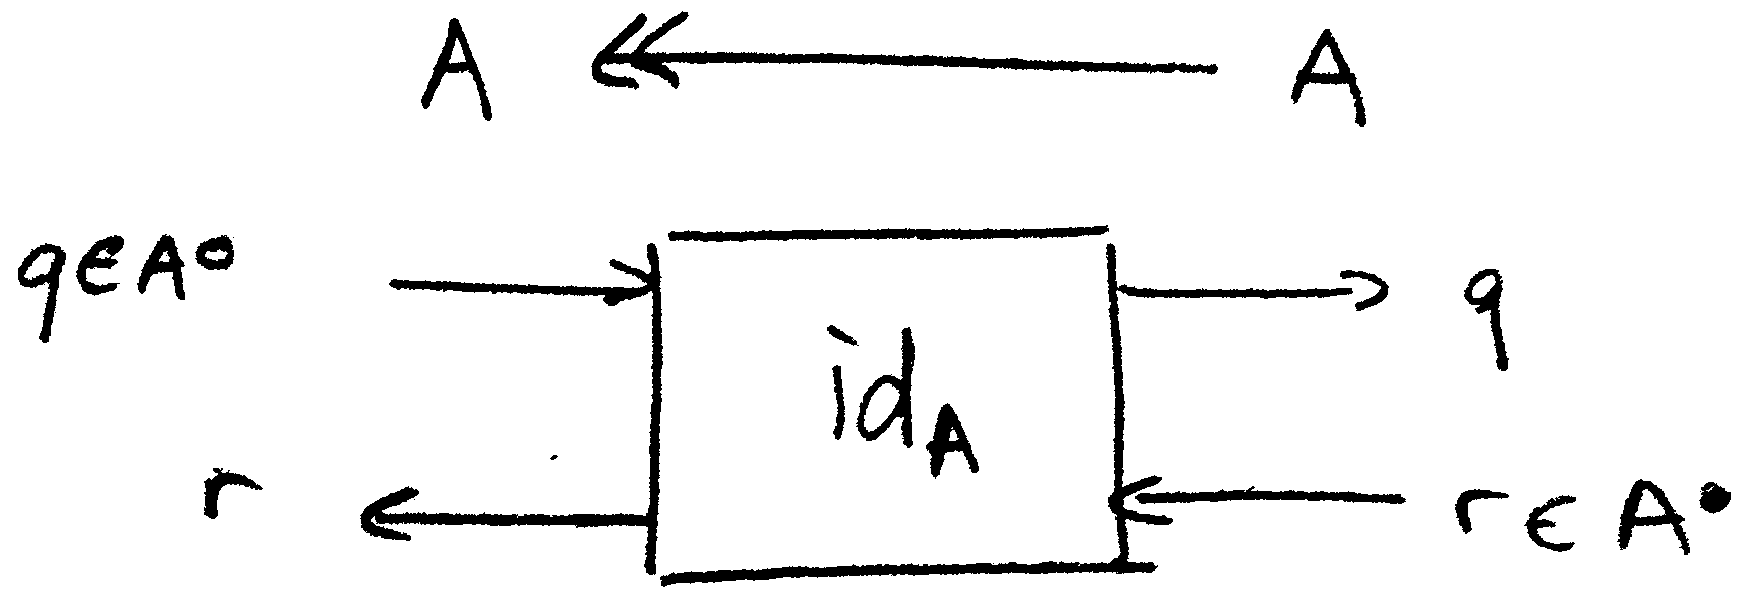
\includegraphics[scale=0.06]{draftfig/identity}
  \]
  \caption{Informal description of CompCertO's transition systems
    and their composition}  
  \label{fig:overview:ts}
\end{figure}
%}}}

\begin{figure} % fig:code {{{
  \centering\footnotesize
  \begin{subfigure}{0.45\textwidth}
\begin{minted}{C}
/* Encapsulated state */
static int c1, c2;
static V buf[N];

/* Accessors */
int inc1() { int i = c1++; c1 %= N; return i; }
int inc2() { int i = c2++; c2 %= N; return i; }
V get(int i) { return buf[i]; }
void set(int i, V val) { buf[i] = val; }
\end{minted}
  \subcaption{The translation unit $\kw{rb.c}$}
  \label{fig:rb}
  \end{subfigure}
  \hspace{4em}
  \begin{subfigure}{0.38\textwidth}
\begin{minted}{C}
/* Underlay signature */
extern int inc1(void);
extern int inc2(void);
extern V get(int i);
extern void set(int i, V val);

/* Layer implementation */
void enq(V val) { set(inc2(), val); }
V deq() { return get(inc1()); }
\end{minted}
  \subcaption{The translation unit $\kw{bq.c}$}
  \label{fig:bq}
  \end{subfigure}
  \caption{Running example, consisting of two C components.
    The component $\kw{rb.c}$
    implements a ring buffer by encapsulating an array
    and two counters. It is used by the component
    $\kw{bq.c}$ to implement a
    bounded queue.}
  \label{fig:code}
%\caption{The state of a ring buffer,
%  made of two counters and a fixed-size array,
%  is encapsulated behind a simple interface.}
%\label{fig:rb}
%\caption{This component relies on the ring buffer primitives
%  provided in Fig.~\ref{fig:rb} to implement a bounded-size queue.}
%\label{fig:bq}
\end{figure}
%}}}

\paragraph{Transition Systems} %{{{

We describe CompCertO's transition systems in detail in \S\ref{sec:base}.
For now, it suffices to note that
a transition system of type $A \twoheadrightarrow B$
describes a behavior of the shape depicted in Fig.~\ref{fig:overview:ts}a,
generating interaction traces of the following form:
\[
  q \rightarrowtail q_1 \leadsto r_1
    \rightarrowtail \cdots \rightarrowtail q_n \leadsto r_n
    \rightarrowtail r
\]
Here, $\rightarrowtail$ denotes internal execution
and $\leadsto$ denotes a step where the environment is in control:
The component is activated by an incoming call,
described by a question $q \in B^\que$.
%which is used to determine the transition system's initial state.
As it executes,
the transition system may perform outgoing calls,
asking questions
$q_1, \ldots, q_n \in A^\que$
and receiving corresponding answers
$r_1, \ldots, r_n \in A^\ans$.
Execution terminates with
the top-level answer $r \in B^\ans$.

\begin{example}[Clight semantics] \label{ex:clightsem} %{{{
CompCertO defines
the semantics of a C translation unit $M$
as:
\[
  \kw{Clight}(M) :
    \mathcal{C} \mathbin@ \kw{mem} \twoheadrightarrow
    \mathcal{C} \mathbin@ \kw{mem}
\]
%Note that both incoming and outgoing call
%use the same language interface $\mathcal{C}_\kw{m}$.
%
Consider the translation unit $\kw{rb.c}$ shown in Fig.~\ref{fig:code}.
If $\kw{inc1}()$ is invoked
with a memory state where the variable $\kw{c1}$ has value $5$,
the transition system $\kw{Clight}(\kw{rb.c})$ will behave as follows:
\[
  \kw{inc1}()@m[\kw{c1} \mapsto 5]
  \: \rightarrowtail \:
  5@m[\kw{c1} \mapsto 6]
\]
Note that the memory is updated to store the new value of the counter $\kw{c1}$.
By contrast, the function $\kw{deq}$ in $\kw{bq.c}$
does not directly modify the memory,
but it makes calls into $\kw{rb.c}$ which may have this effect.
The corresponding executions of $\kw{Clight}(\kw{bq.c})$
will have the shape
\[
  \kw{deq}()@m
  \rightarrowtail
  \kw{inc1}()@m \leadsto i@m'
  \rightarrowtail
  \kw{get}(i)@m' \leadsto v@m''
  \rightarrowtail
  v@m''
  \,.
\]
\end{example}
%}}}

%}}}

\paragraph{Composition} %{{{

Transition systems can be composed in different ways.
To model \emph{linking}, the original work on CompCertO introduces an operator
\[
  {\oplus}_A : (A \twoheadrightarrow A) \times (A \twoheadrightarrow A)
  \rightarrow (A \twoheadrightarrow A)
  \,.
\]
This operator allows mutual recursion:
in $L_1 \oplus L_2$, both
outgoing calls of $L_1$ to functions of $L_2$ and
outgoing calls of $L_2$ to functions of $L_1$
become internal calls and are hidden from the environment.

When mutual recursion is not needed,
we can use a more traditional and flexible operator
\[
  {\odot}_{A,B,C} :
    (B \twoheadrightarrow C) \times
    (A \twoheadrightarrow B) \rightarrow
    (A \twoheadrightarrow C)
  \,.
\]
Here,
the transition systems interact only over
the language interface $B$,
so that in $L_1 \odot L_2$,
incoming calls activate $L_1$ in $C$,
the outgoing calls of $L_1$ in $B$ are handled by $L_2$, and
the outgoing calls of $L_2$
are directed back to the environment in $C$.
This is depicted in Fig.~\ref{fig:overview:ts}b.

This mode of composition was hinted at in \citet{compcerto}.
We provide a formal definition in \S\ref{sec:basic:lcomp}
and show that
it defines a category $\mathbf{TS}$ of
language interfaces and transition systems.
In particular,
the unit for $\odot$ is
the transition system $\kw{id}_A : A \twoheadrightarrow A$
depicted in Fig.~\ref{fig:overview:ts}c,
which echoes the incoming question as an outgoing one
and propagates the answer back to the caller.

%}}}

%}}}

\subsection{Adjoining State} \label{sec:overview:slift} %{{{

\subsubsection{Language Interfaces} %{{{

We have seen that CompCertO
requires the current memory state to be attached
to every question and answer,
and used the notation $\mathcal{C} \mathbin@ \kw{mem}$
to describe the resulting language interface.
This can be generalized to arbitrary
language interfaces and sets of states:
\[
  A \mathbin@ U \: := \:
    \langle A^\que \times U, \: A^\ans \times U \rangle
\]
Taking a cue from \citep{rbgs-cal},
this allows \emph{certified abstraction layers} to be modeled
within the CompCertO framework.

%}}}

\begin{example}[Certified Abstraction Layers] \label{ex:overview:lint} %{{{

Software systems are often constructed in layers:
basic data structures and functionality
are implemented by low-level code.
We can then rely on this code
without concern its implementation details
or the data representation it uses.
Instead,
a programmer writing client code
will understand and reason about
this layer of code
in terms of a more abstract mental picture
of its operation.
For example,
when using the functions $\kw{enq}$ and $\kw{deq}$
shown in Fig.~\ref{fig:code},
we can think of the bounded queue they provide
as a simple sequence of elements,
and ignore the mechanics
of the ring buffer used to implement it.
\emph{Certified abstraction layers}
formalize this methodology within CompCert
and were used to verify the operating system kernel
CertiKOS \cite{popl15}.

Modeling layers required a modification of CompCert's semantics
to incorporate an \emph{underlay interface}
described using an \emph{abstract state}.
%to achieve a limited form of compositionality.
The closed semantics of CompCert can be described as
\[
  \chi : \top \twoheadrightarrow \mathcal{C} \mathbin@ \kw{mem}
  \: \vdash \:
  \kw{Clight}_\chi[M] : \top \twoheadrightarrow \mathbf{I}
  \,,
  \quad \text{ where }
  \top := \langle \varnothing, \varnothing \rangle
  \text{ and }
  \mathbf{I} := \langle \mathbbm1, \mathbbm1 \rangle
  \,.
\]
The transition system $\kw{Clight}_\chi[M]$
is invoked with a trivial question ${*} \in \mathbf{I}^\que$,
which initiates the execution of the $\kw{main}$ function of $M$.
When $M$ invokes an external function,
the behavior of that function is obtained from the parameter $\chi$.
In the CertiKOS proof,
abstraction layers are formalized by using
a variant CompCertX,
whose semantic model can be described as:
\[
  \forall D \in \mathbf{Set}
  \: \mathbin. \:
  L^\flat :
    \top \twoheadrightarrow
    \mathcal{C} \mathbin@ \kw{mem} \mathbin@ D
  \: \vdash \:
  \kw{Clight}_{L^\flat}[M] :
    \top \twoheadrightarrow
    \mathcal{C} \mathbin@ \kw{mem} \mathbin@ D
  \,.
\]
This allows the semantics of $M$ to be evaluated
in the context of the \emph{underlay} interface $L^\flat$,
whose primitives are described in terms of
an \emph{abstract state} memory component of type $D$.
A specification for the code in \autoref{fig:code}
may use an abstract state in $S_\kw{bq} := \kw{val}^*$.
The corresponding layer interface
$L_\kw{bq} : \top \twoheadrightarrow
 \mathcal{C} \mathbin@ \kw{mem} \mathbin@ S_\kw{bq}$
will then generate traces such as:
\[
  L_\kw{bq} \:\vDash\:
  \kw{enq}(v) \mathbin@ m \mathbin@ \vec{q}
  \:\rightarrowtail\:
  \kw{undef} \mathbin@ m \mathbin@ \vec{q}v
  \qquad%\qquad
  L_\kw{bq} \:\vDash\:
  \kw{deq}() \mathbin@ m \mathbin@ v\vec{q}
  \:\rightarrowtail\:
  v \mathbin@ m \mathbin@ \vec{q}
\]
We can then evaluate and reason about any client code
in terms of this abstract representation:
\[
  \kw{Clight}_{L_\kw{bq}} \big[\,
  \begin{minipage}{13em}
\begin{minted}{C}
void rot() { enq(deq()); }
\end{minted}
  \end{minipage} \,\big]
\:\vDash\:
%  \qquad
%  \Rightarrow
%  \qquad
  \kw{rot}() \mathbin@ m \mathbin@ v\vec{q}
  \:\rightarrowtail\:
  {*} \mathbin@ m \mathbin@ \vec{q}v
  \,.
\]

We will use certified abstraction layers
to illustrate the flexibility of CompCertO's approach
and as an example application for the techniques we introduce.
\end{example}
%}}}

\subsubsection{Transition Systems} \label{sec:overview:slift:ts} %{{{

In the example above,
the client code $M$ does not directly access
the abstract memory component $\vec{q}$, % in $D$,
and can only affect it by invoking
the primitives of the underlay interface $L_\kw{bq}$.
In our compositional framework,
a transition system
$L : A \twoheadrightarrow B$,
can be extended to
\[
  L \mathbin@ U : A \mathbin@ U \twoheadrightarrow B \mathbin@ U
  \,.
\]
The transition system $L \mathbin@ U$ transparently passes along
a state component of type $U$ as follows:
\begin{equation} \label{eqn:slift}
  \begin{prooftree}
  \hypo{
  L \:\vDash\: q \rightarrowtail
    q_1 \leadsto r_1 \rightarrowtail
    \cdots \rightarrowtail
    q_n \leadsto r_n \rightarrowtail
    r
  }
  \infer1{
  L \mathbin@ U \:\vDash\: q@u_0 \rightarrowtail
    q_1@u_0 \leadsto r_1@u_1 \rightarrowtail
    \cdots \rightarrowtail
    q_n@u_{n-1} \leadsto r_n@u_n \rightarrowtail
    r@u_n
  }
  \end{prooftree}
\end{equation}
Here, the value $u_0 \in U$
is initially received from the environment as part of the incoming question.
$L \mathbin@ U$ then mirrors the execution of $L$
but keeps track of this additional state component.
The state is attached to any outgoing question in $A$
and updated when the corresponding answer is received.
When $L$ terminates,
the final value of the state is returned with the answer in $B$.

\begin{example}[Layer Semantics] %{{{
As noted in Example~\ref{ex:overview:lint},
the CertiKOS verification effort
required the entire correctness proof of CompCert
to be modified to operate in terms of an underlay interface.
We can achieve a similar effect in CompCertO
without any modification to the compiler,
by defining
\[
  \kw{Clight}_{L^\flat}[M] :=
    (\kw{Clight}(M) \mathbin@ D^\flat) \odot L^\flat
  \,.
\]
We will see that CompCertO's open simulations
make it possible to formulate layer correctness
in a reasonably straightforward way as well.
\end{example}

%Using this construction,
%a C layer interface $L^\flat$ which uses abstract states in $D$
%can be modeled as a transition system of type
%$
%  L^\flat : \top \twoheadrightarrow \mathcal{C}_\kw{m}@D
%$,
%using questions and answers of the form:
%\begin{align*}
%  (\mathcal{C}_\kw{m}@D)^\que &:=
%    \{ f(\vec{v})@(m, d) \mid
%       f \in \kw{ident},
%       \vec{v} \in \kw{val}^*,
%       m \in \kw{mem},
%       d \in D \}
%  \\
%  (\mathcal{C}_\kw{m}@D)^\ans &:=
%    \{ v'@(m', d') \mid
%       v' \in \kw{val},
%       m' \in \kw{mem},
%       d' \in D \}
%\end{align*}
%This leaves the question of evaluating client code
%running on top of the underlay $L$.
%}}}

%}}}

%}}}

\subsection{Simulations} %{{{

% Simulation basics {{{

CompCert establishes compiler correctness
as a simulation property
\[
  \kw{CompCert}(M) = M'
  \quad\Rightarrow\quad
  \kw{Clight}_\chi[M] \:\le\: \kw{Asm}_\chi[M']
  \,.
\]
This means that when $M$ compiles to $M'$,
the behavior of the source program $M$
is simulated by the behavior of $M'$.
The transitivity of simulations enables
\emph{vertical compositionality}:
the overall correctness of the compiler
can be derived from that of
individual compilation passes.

In CompCertO,
correctness is formulated at the level of
individual components.
When $M$ is compiled to $M'$,
we must establish a relationship between
the open transition systems
\[
  \kw{Clight}(M) :
    \mathcal{C} \mathbin@ \kw{mem} \twoheadrightarrow
    \mathcal{C} \mathbin@ \kw{mem}
  \qquad \text{and} \qquad
  \kw{Asm}(M') :
    \mathcal{A} \mathbin@ \kw{mem} \twoheadrightarrow
    \mathcal{A} \mathbin@ \kw{mem}
  \,.
\]
This raises the question of the relationship
between the source-level interactions
in $\mathcal{C} \mathbin@ \kw{mem}$
and their corresponding target-level interactions
in $\mathcal{A} \mathbin@ \kw{mem}$.
In other words,
compositional compiler correctness only makes sense
with respect to a particular calling convention.

\paragraph{Simulation Conventions}

%Rather than modeling the calling convention implicitly
%as part of the assembly semantics,
CompCertO makes this explicit:
simulations operate in the context of specified
\emph{simulation conventions}.
%which express the relationships between
%the source and target components'
%interactions with the environment.
%
This introduces a form of two-dimensional typing.
To establish a simulation
of a transition system $L^\sharp: A^\sharp \twoheadrightarrow B^\sharp$
by a transition system $L^\flat: A^\flat \twoheadrightarrow B^\flat$,
we must first specify a simulation convention
$\mathbb{R}_B : B^\sharp \Leftrightarrow B^\flat$
for their incoming calls,
and a simulation convention
$\mathbb{R}_A : A^\sharp \Leftrightarrow A^\flat$
for their outgoing calls.
We can depict this situation
in the following ways:
\[
  \begin{tikzcd}
    A^\sharp
      \ar[r, twoheadrightarrow, "L^\sharp"]
      \ar[d, Leftrightarrow, "\mathbb{R}_A"'] &
    B^\sharp
      \ar[d, Leftrightarrow, "\mathbb{R}_B"] \\
    A^\flat
      \ar[r, twoheadrightarrow, "L^\flat"'] &
    B^\flat
  \end{tikzcd}
  \qquad \qquad
  L^\sharp \le_{\mathbb{R}_A \twoheadrightarrow \mathbb{R}_B} L^\flat
  \qquad \qquad
  \vcenter{ \hbox{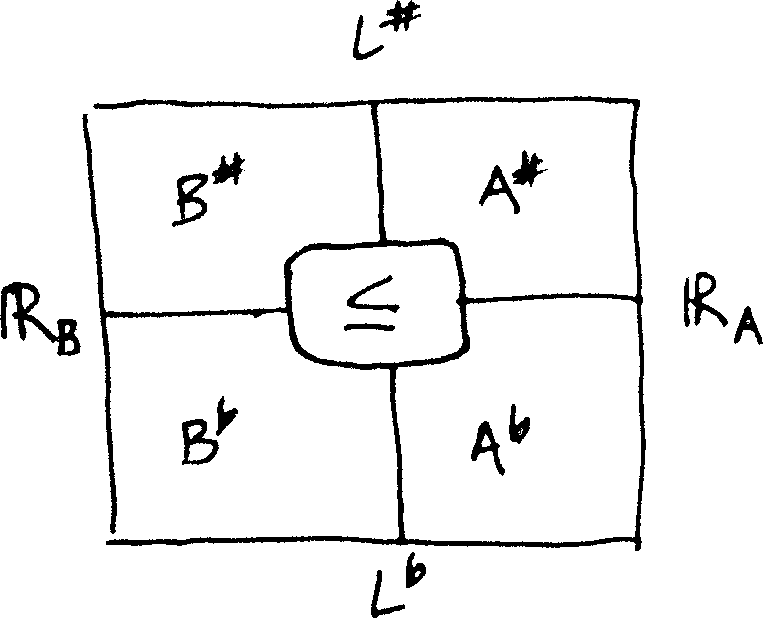
\includegraphics[scale=0.095]{draftfig/simsd}} }
\]
Simulation conventions are relational in nature.
Given $\mathbb{R} : A \Leftrightarrow B$ and
$\mathbb{R}' : B \Leftrightarrow C$,
we can derive their sequential composition
$\mathbb{R} \cdot \mathbb{R}' : A \Leftrightarrow C$.
We will write $\epsilon_A : A \Leftrightarrow A$
for the identity simulation convention,
and call $\mathbf{SC}$ the associated category of
language interfaces and simulation conventions.

%}}}

\begin{figure} % fig:overview:simcomp %{{{
  \[
      \pi_1 :
        L_1^\sharp
        \le_{\mathbb{R}_B \cdot \mathbb{R}_B' \twoheadrightarrow
             \mathbb{R}_C}
        L_1^\flat
      \qquad
      \pi_2 :
        L_2^\sharp
        \le_{\mathbb{R}_A \twoheadrightarrow \mathbb{R}_B}
        L_2^\natural
      \qquad
      \pi_2' :
        L_2^\natural
        \le_{\mathbb{R}_A' \twoheadrightarrow \mathbb{R}_B'}
        L_2^\flat
  \]
  \[
    \begin{tikzcd}[row sep=1.5em]
      A^\sharp \ar[r, twoheadrightarrow, "L_2^\sharp"]
	       \ar[d, Leftrightarrow, "\mathbb{R}_A"'] &
      B^\sharp \ar[r, twoheadrightarrow, "L_1^\sharp"]
               \ar[d, Leftrightarrow, "\mathbb{R}_B"] &
      C^\sharp \ar[dd, Leftrightarrow, "\mathbb{R}_C"]
      \\
      A^\natural \ar[r, twoheadrightarrow, "L_2^\natural"]
	       \ar[d, Leftrightarrow, "\mathbb{R}'_A"'] &
      B^\natural \ar[d, Leftrightarrow, "\mathbb{R}'_B"]
      \\
      A^\flat \ar[r, twoheadrightarrow, "L_2^\flat"] &
      B^\flat \ar[r, twoheadrightarrow, "L_1^\flat"] &
      C^\flat
    \end{tikzcd}
    \qquad
    \begin{prooftree}
      \hypo{\pi_1 \quad}
      \hypo{\pi_2 \quad}
      \hypo{\quad \pi_2'}
      \infer2{
	%\pi_2 \odot \pi_2' :
	L_2^\sharp
	\le_{\mathbb{R}_A \cdot \mathbb{R}_A' \twoheadrightarrow
	     \mathbb{R}_B \cdot \mathbb{R}_B'}
	L_2^\flat}
      \infer2{
	%\pi_1 \otimes (\pi_2 \odot \pi_2') :
	L_1^\sharp \odot L_2^\sharp
	\le_{\mathbb{R}_A \cdot \mathbb{R}_A' \twoheadrightarrow
	     \mathbb{R}_C}
	L_1^\flat \odot L_2^\flat}
    \end{prooftree}
    \qquad
    \vcenter{ \hbox{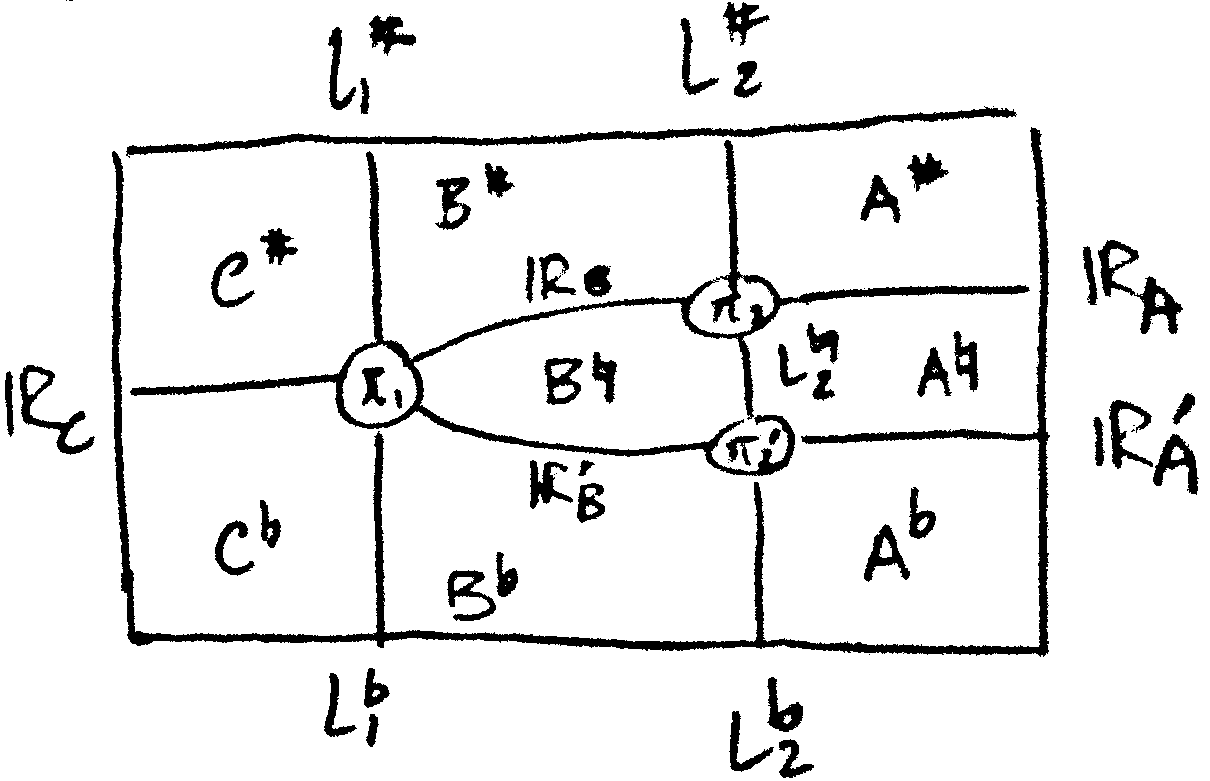
\includegraphics[scale=0.1]{draftfig/simsdcomp}} }
  \]
  \caption{A composite simulation proof
     and associated graphical representations}
  \label{fig:overview:simcomp}
\end{figure}
%}}}

\paragraph{Composition Properties} %{{{

As illustrated in Fig.~\ref{fig:overview:simcomp},
when their boundaries are compatible,
simulation squares of the kind depicted above compose both
vertically and horizontally.
Vertical composition produces a simulation
which uses the sequential composition
of its components' simulation conventions.
Horizontal composition produces a simulation
between the composite source and target components.

Our work builds on this framework in various directions.
First,
we formulate horizontal composition in terms of
the layered composition $\odot$.
As suggested in \citet{compcerto},
this formally equips language interfaces,
transition systems and
simulation conventions
with the structure of a double category.
Secondly,
we make simulation conventions more expressive
by allowing them to retain a form of \emph{state},
allowing them to relate successive interactions
in different ways.
Finally,
we carry through the approach initiated in \S\ref{sec:overview:slift}
to its conclusion
by making explicit the compositional structure of
language interfaces themselves,
allowing transition systems and simulation conventions
to operate independently on their different components.

%}}}

%\begin{color}{gray}
%Simulations are compatible with our composition operator $\odot$.
%In other words, the following \emph{horizontal} composition property holds
%(\autoref{thm:lcompsim}):
%\[
%  \begin{tikzcd}
%    A^\sharp \ar[r, twoheadrightarrow, "L_2^\sharp"]
%             \ar[d, Leftrightarrow, "\mathbb{R}_A"] &
%    B^\sharp \ar[r, twoheadrightarrow, "L_1^\sharp"]
%             \ar[d, Leftrightarrow, "\mathbb{R}_B"] &
%    C^\sharp \ar[d, Leftrightarrow, "\mathbb{R}_C"]
%    \\
%    A^\flat \ar[r, twoheadrightarrow, "L_2^\flat"'] &
%    B^\flat \ar[r, twoheadrightarrow, "L_1^\flat"'] &
%    C^\flat
%  \end{tikzcd}
%  \qquad \Longrightarrow \qquad
%  \begin{tikzcd}
%    A^\sharp \ar[rr, twoheadrightarrow, "L_1^\sharp \odot L_2^\sharp"]
%             \ar[d, Leftrightarrow, "\mathbb{R}_A"'] & &
%    C^\sharp \ar[d, Leftrightarrow, "\mathbb{R}_C"]
%    \\
%    A^\flat \ar[rr, twoheadrightarrow, "L_2^\flat \odot L_1^\flat"'] & &
%    C^\flat
%  \end{tikzcd}
%\]
%Simulations also admit a \emph{vertical} composition property,
%which for example allows CompCertO's correctness theorem
%to be derived from the correctness proofs of
%individual compilation passes:
%\[
%  \begin{tikzcd}[row sep=1.5em]
%    A^\sharp \ar[r, twoheadrightarrow, "L^\sharp"]
%	     \ar[d, Leftrightarrow, "\mathbb{R}_A"'] &
%    B^\sharp \ar[d, Leftrightarrow, "\mathbb{R}_B"]
%    \\
%    A^\natural \ar[r, twoheadrightarrow, "L^\natural"]
%	     \ar[d, Leftrightarrow, "\mathbb{S}_A"'] &
%    B^\natural \ar[d, Leftrightarrow, "\mathbb{S}_B"]
%    \\
%    A^\flat \ar[r, twoheadrightarrow, "L^\flat"] &
%    B^\flat
%  \end{tikzcd}
%  \qquad \Longrightarrow \qquad
%  \begin{tikzcd}
%    A^\sharp \ar[r, twoheadrightarrow, "L^\sharp"]
%             \ar[dd, Leftrightarrow, "\mathbb{R}_A \cdot \mathbb{S}_A"'] &
%    B^\sharp \ar[dd, Leftrightarrow, "\mathbb{R}_B \cdot \mathbb{S}_B"] \\ \\
%    A^\flat \ar[r, twoheadrightarrow, "L^\flat"'] &
%    B^\flat
%  \end{tikzcd}
%\]
%Here,
%the simulation convention composition operator $\mathbb{R} \cdot \mathbb{S}$
%roughly corresponds to relational composition.
%Together,
%these structures and properties
%extend language interfaces and transition systems
%with the structure of a \emph{double category}.
%This is made precise in \S\ref{sec:base}.
%\end{color}

%}}}

\subsection{Monoidal Structures} %{{{

We introduced in \S\ref{sec:overview:slift}
the constructions $A \mathbin@ U$ and $L \mathbin@ U$
which extend the language interface $A$ and transition system $L$
with an additional state component taken in the set $U$.
This construction can be decomposed further
and extended to simulation conventions.

\begin{definition}[Composite language interfaces] %{{{
Given two language interfaces $A$ and $B$,
the language interface $A \otimes B$ is defined as:
$
  A \otimes B :=
    \langle A^\que \times B^\que, \,
            A^\ans \times B^\ans \rangle
$.
The language interface
$\mathbf{I} = \langle \mathbbm{1}, \mathbbm{1} \rangle$
is a unit for $\otimes$.
In addition, for a set $U$
we define the language interface
$[U] := \langle U, U \rangle$.
\end{definition}
%}}}

We can recover
$A \mathbin@ U := A \otimes [U]$.
Note also that $\otimes$ is %(in essence)
associative and commutative,
and that:
\[
  [U \times V] = [U] \otimes [V]
  \qquad \qquad
  [\mathbbm{1}] = \mathbf{I}
  \qquad
  [\varnothing] = \top
\]
Moreover,
the underlying structures
are mirrored at the level of simulation conventions.

\paragraph{Simulation Conventions} %{{{

Two simulation conventions
$\mathbb{R} : A^\sharp \Leftrightarrow A^\flat$ and
$\mathbb{S} : B^\sharp \Leftrightarrow B^\flat$
can be combined into %a simulation convention
$
  \mathbb{R} \otimes \mathbb{S} :
  A^\sharp \otimes B^\sharp \Leftrightarrow
  A^\flat \otimes B^\flat
$.
This simulation convention
(Def.~\ref{def:sctens})
requires the $A$ and $B$ components
of questions and answers
to be related independently by $\mathbb{R}$ and $\mathbb{S}$.
In addition,
a relation $R \subseteq U^\sharp \times U^\flat$
can be promoted to a simulation convention
$
  [R] : [U^\sharp] \Leftrightarrow [U^\flat]
$
which uses $R$ as the underlying relation for both
questions and answers.

These constructions satisfy many properties
which are well-understood in the context of category theory.
For example, the properties
\[
  \epsilon_A \otimes \epsilon_B = \epsilon_{A \otimes B}
  \qquad \text{and}
  \qquad
  (\mathbb{R}_1 \otimes \mathbb{R}_2) \cdot
  (\mathbb{S}_1 \otimes \mathbb{S}_2) =
  (\mathbb{R}_1 \cdot \mathbb{S}_1) \otimes
  (\mathbb{R}_2 \cdot \mathbb{S}_2)
  \,,
\]
and various properties of the invertible simulation conventions:
\[
  \lambda_A : A \otimes \mathbf{I} \cong A \,,
  \qquad
  \alpha_{ABC} : (A \otimes B) \otimes C \cong A \otimes (B \otimes C) \,,
  \qquad
  \gamma_{AB} : A \otimes B \cong B \otimes A \,,
\]
equip %the category
$\mathbf{SC}$
%of language interfaces and simulation conventions
with the structure of a \emph{symmetric monoidal category}.
Likewise, the properties
\[
  [{=}_U] = \epsilon_{[U]} \,,
  \qquad
  [R \mathbin; S] = [R] \cdot [S] \,,
  \qquad
  [R \times S] = [R] \otimes [S]
\]
can be captured by describing
$[-] : \mathbf{Rel} \rightarrow \mathbf{SC}$
as a \emph{monoidal functor}
from the symmetric monoidal category $\mathbf{Rel}$
of sets and relations
to the symmetric monoidal category $\mathbf{SC}$.

%This categorical description %of the compositional structure
%of simulation conventions
%brings with it useful tools.
%In essence,
Symmetric monoidal categories capture
the algebra of systems or processes which
compose both in series and parallel
\cite{rosetta}.
In the case of simulation conventions,
the process is one of concretization
from a high-level, abstract representation
of component interactions
to a more concrete and low-level one.
Series composition ($\cdot$)
allows us to carry out this process in a stepwise manner,
while parallel composition ($\otimes$)
allows us to operate independently on various components
of questions and answers.
Category theory backs this intuition
with a number of formal tools;
we will make extensive use of \emph{string diagrams}
when describing complex simulation conventions.

%}}}

\paragraph{String Diagrams} %{{{

As implied by the properties above,
a composite morphism in a symmetric monoidal category
can often be written in a variety of equivalent ways.
String diagrams provide a more economical representation,
where these equivalences are captured
by simple geometric intuition.
For example, consider the following situation:
\[
  \begin{prooftree}
    \hypo{
      \begin{array}{c}
	w : A \Leftrightarrow B \\
	x : \mathbf{I} \Leftrightarrow C \\
	y : C \Leftrightarrow D \\
	z : B \otimes D \Leftrightarrow E
      \end{array}
    }
    \infer1{\mathbb{R} : A \Leftrightarrow E}
  \end{prooftree}
  \quad
  \begin{array}{r@{}l}
    \mathbb{R} := {} &
    \lambda_A^{-1} \cdot
    (A \otimes x) \cdot
    (w \otimes y) \cdot
    z 
    \\[0.5ex]
    = {} &
    \lambda_A^{-1} \cdot
    (w \otimes (x \cdot y)) \cdot z
    \\[0.5ex]
    = {} &
    w \cdot \lambda_B^{-1} \cdot
    (B \otimes (x \cdot y)) \cdot z
    \\
    \vdots \:\, &
  \end{array}
  \qquad\qquad
  \mathbb{R} := \:\vcenter{\hbox{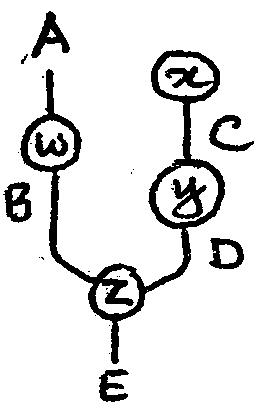
\includegraphics[scale=0.15]{draftfig/sdexample}} }
\]
Here,
we define a simulation convention $\mathbb{R}$ from various components
using categorical operations.
On the left,
we show the type of every variable,
and give several equivalent definitions for $\mathbb{R}$.
The string diagram on the right
captures the same information
in a more compact and readable way.
Note that string diagrams
are \emph{formal} diagrams,
which denote a particular morphism
with the same degree of rigor
as traditional mathematical notation.

The string diagrams we use to represent simulation conventions
can be read from top to bottom.
Vertical lines denote language interfaces,
and horizontal juxtaposition represent tensor products.
Since it is the unit for $\otimes$,
the language interface $\mathbf{I}$ is not explicitly represented.
Nodes connect a group of lines above to a group of lines below
and denote elementary simulation conventions,
and are connected vertically to denote sequential composition.
Like the language interface $\mathbf{I}$,
the identity simulation convention $\epsilon$ is omitted,
and may appear as a vertical line without an intervening node.
Based on these conventions,
the string diagram above can be read as:
\newcommand{\chunk}[1]{%
  \vcenter{\hbox{%
    \includegraphics[scale=0.1]{draftfig/sd/#1}%
  }}%
}
\begin{align*}
  \mathbb{R}
     = \chunk{l1} \cdot \chunk{l2} \cdot \chunk{l3}
    &= \lambda_A^{-1} \cdot
       \left( \chunk{c1} \otimes \chunk{c2} \right) \cdot
       \left( \chunk{c3} \otimes \chunk{c4} \right) \cdot
       \chunk{c5} \\
    &= \lambda_A^{-1} \cdot (\epsilon_A \otimes x) \cdot (w \otimes y) \cdot z
    \,.
\end{align*}
There are other ways to decompose the diagram,
which yield some of the alternate formulas for $\mathbb{R}$
shown above.
But conversely,
the string diagrams representations of these formulas
are all identical,
up to topological deformations
which correspond to the axioms of monoidal categories.

\begin{example}[Abstraction Relations] \label{ex:overview:absrel} %{{{
In \S\ref{sec:overview:slift},
we noted that a layer specification
$L^\sharp :
 \top \twoheadrightarrow \mathcal{C} \mathbin@ \kw{mem} \mathbin@ D^\sharp$
and its implementation
$\kw{Clight}_{L^\flat}[M] :
 \top \twoheadrightarrow \mathcal{C}_\kw{m}@D^\flat$
%in terms of an underlay $L^\flat$
are not directly comparable, owing to their
use of different abstract states.
We now show how to construct,
using the techniques that we have introduced,
a simulation convention suitable for
stating the desired correctness property.

Note the decomposition
$\mathcal{C}_\kw{m}@D \cong \mathcal{C} \otimes [\kw{mem}] \otimes [D]$.
When a layer specification $L^\sharp$ is implemented,
part of its abstract state $D^\sharp$ is realized as concrete values
stored in the global memory,
and part of it reflects the abstract state of the underlay in $D^\flat$.
The details of this can be expressed using a relation
$R \subseteq (\kw{mem} \times D^\sharp) \times (\kw{mem} \times D^\flat)$,
allowing us to state the layer correctness property as
\[
  L^\flat \vdash_R M : L^\sharp \quad :\Leftrightarrow \quad
    L^\sharp \le_{\top \twoheadrightarrow \mathcal{C} \otimes [R]}
    \llbracket M \rrbracket_{L^\flat}
  \,.
\]
To ensure that this relation is compatible with client code,
we must require that
\[
  \forall C \mathbin.
    \kw{Clight}(C)@D^\sharp
    \le_{\mathcal{C} \otimes [R] \twoheadrightarrow \mathcal{C} \otimes [R]}
    \kw{Clight}(C)@D^\flat
  \,.
\]
%Now consider an assembly version
%$L^\sharp_\mathcal{A} :
% \top \twoheadrightarrow \mathcal{A} \otimes [\kw{mem}] \otimes [D^\sharp]$
%of the specification, such that
%\[
%  L^\sharp
%  \le_{\top \twoheadrightarrow \mathbb{C} \otimes D^\sharp}
%  L^\sharp_\mathcal{A}
%  \,.
%\]
\end{example}
%}}}

%}}}

\paragraph{Transition Systems} %{{{

Unfortunately,
it is not possible in general
to form the tensor product of transition systems.
To see why, consider a hypothetical product
\[
  L_1 \otimes L_2 : A_1 \otimes A_2 \twoheadrightarrow B_1 \otimes B_2
  \,.
\]
When a question is received in $B_1 \otimes B_2$,
its components in $B_1$ and $B_2$ can be used to activate
the underlying transition systems $L_1$ and $L_2$.
However, during their execution,
each may ask
an arbitrary number of questions in $A_1$ and $A_2$.
In general,
there is no reason to expect that these questions
will synchronize or
that there will be a way to
combine them meaningfully
into questions of $A_1 \otimes A_2$.

Although $\mathbf{TS}$
cannot be made into a symmetric monoidal category,
the state threading construction $L@U$ can be generalized
to allow the added state component
to use different representations in incoming and outgoing questions.
Formally, we define a functor
\[
  \mathbin@ : \mathbf{TS} \times \mathbf{Iso}(\mathbf{Set})
    \rightarrow \mathbf{TS}
\]
which from a transition system $L : A \twoheadrightarrow B$
and a bijection $f : U \cong V$
constructs a transition system
\[
  L \mathbin@ f \::\: A \otimes [U] \:\twoheadrightarrow\: B \otimes [V]
  \,.
\]
The behavior of this transition system is similar to that of $L@U$,
but the bijection $f$ is used to translate the state component
between incoming and outgoing questions.

Since the right-hand side argument of $\mathbin@$
is limited to sets and bijections,
it cannot be used to define a proper monoidal structure on $\mathbf{TS}$.
Nevertheless, there are transition systems
\[
  \lambda^\kw{L}_A : \mathbf{I} \mathbin@ U \cong [U]
  \qquad
  \lambda^\kw{R}_A : A \mathbin@ \mathbbm{1} \cong A
  \qquad
  \alpha_{AUV} : A \mathbin@ (U \times V) \cong
    (A \mathbin@ U) \mathbin@ V
\]
which satisfy a version of the expected properties.
This makes it possible to construct for transition systems
a string diagram language
similar to that of simulation conventions.
For example,
the layer semantics given in \S\ref{sec:overview:slift}
can be written as:
\[
  \kw{Clight}_{L^\flat}[M] \quad:=\quad
    \vcenter{\hbox{ 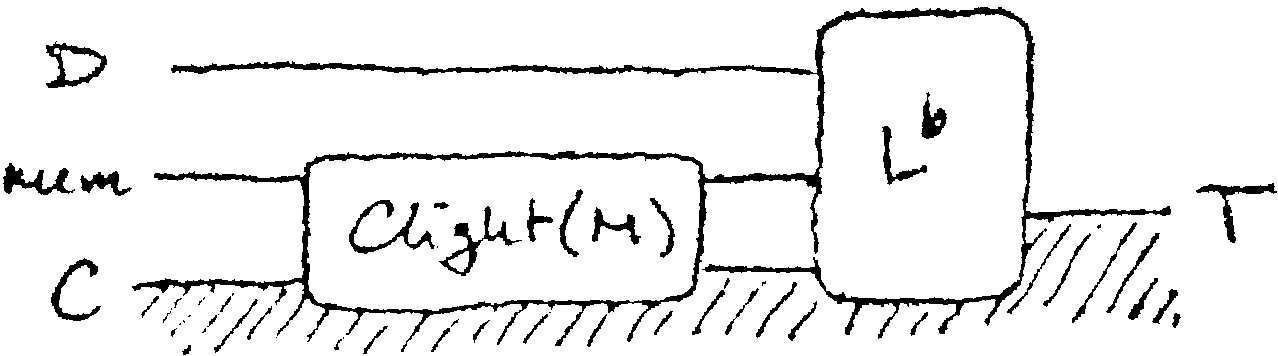
\includegraphics[scale=0.1]{draftfig/layersem} }}
    \quad:\quad
    \top \twoheadrightarrow \mathcal{C} \mathbin@ \kw{mem} \mathbin@ D^\flat
\]
Here,
categorical composition runs from left to right
and the product
$A \mathbin@ U_1 \mathbin@ \cdots \mathbin@ U_n$
run from bottom to top.
Lines and nodes connecting the bottom shaded area
to the rest of the diagram
can be arbitrary language interfaces and transition systems,
but those appearing in the upper part
are restricted to sets and bijections.

\begin{example}[Pure Layer Interfaces] %{{{
In many layer specifications,
the primitives only access and modify the abstract state,
and do not use the concrete memory component at all.
In such cases,
it suffices to define them using the type
$L : \top \twoheadrightarrow \mathcal{C} \mathbin@ D$.
Evaluating client code can then be done as:
\begin{align*}
  \kw{Clight}_{L}[M] \quad&:=\quad
    \vcenter{\hbox{ 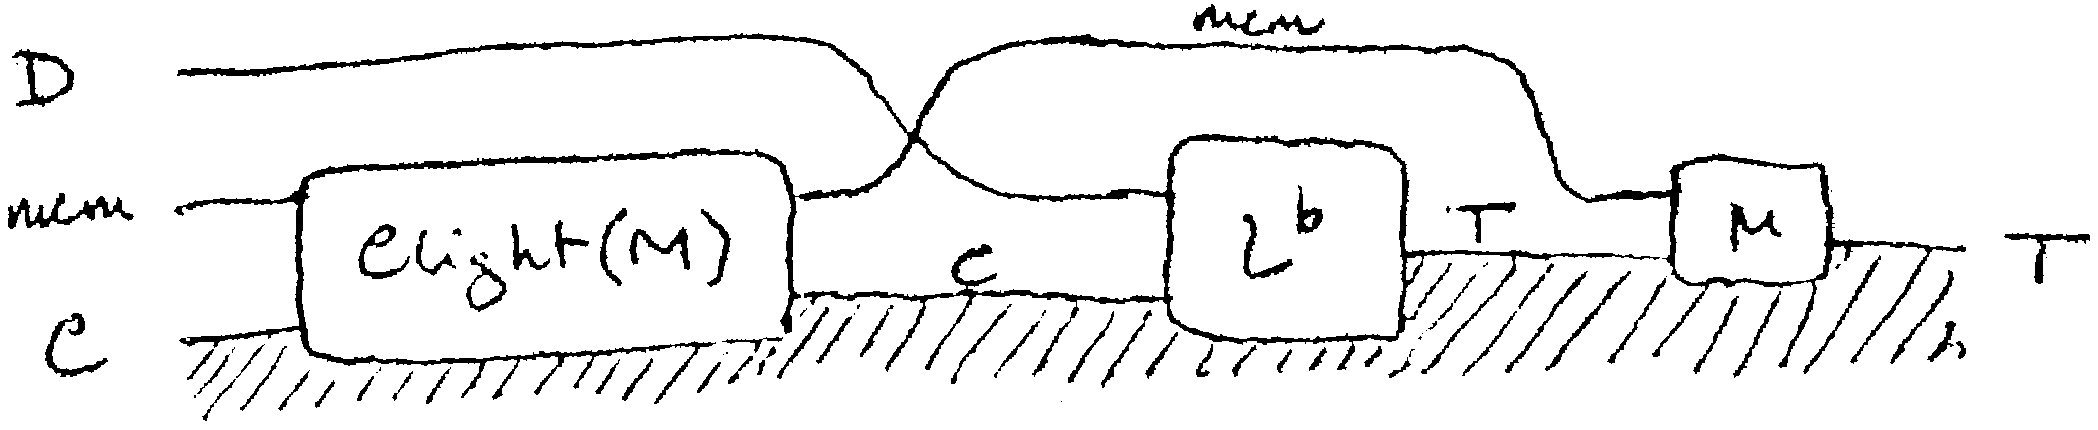
\includegraphics[scale=0.1]{draftfig/layersem-pure} }}
  \\[1ex]
  \quad&\,=\:\: {}
     (\kw{Clight}(M) \mathbin@ D) \odot
     (\mathcal{C} \mathbin@ \gamma_{\kw{mem}, D}) \odot
     (L \mathbin@ \kw{mem}) \odot
     \mu_\kw{mem}
\end{align*}
We have used the isomorphisms
$\gamma_{UV} : U \times V \cong V \times U \in \mathbf{Iso}(\mathbf{Set})$,
represented by a twist in the diagram above,
and $\mu_U : \top \cong \top \mathbin@ U \in \mathbf{TS}$.
\end{example}
%}}}

%}}}

%}}}

\subsection{Separation Algebra} \label{sec:overview:sepalg} %{{{

The constructions we have outlined so far
make it possible to describe
the state of complex systems compositionally.
State can separated into different fields;
we can then describe and reason about individual components
independently of the fields that they do not access,
and use the $\mathbin@$ operator
to connect these components with the rest of the system.

This compositional description
facilitates local reasoning,
but it must eventually be refined into
a concrete implementation:
a program acting on a global memory state.
To establish correctness,
we must formulate a simulation convention
describing the ways in which
the global memory state encodes
the various abstract state components.
To achieve this in a way which preserves compositionality,
we use a \emph{separation algebra}
for the CompCert memory model.

%This process was touched on in Example~\ref{ex:overview:absrel},
%where an abstraction relation
%$R \subseteq (\kw{mem} \times D^\sharp) \times (\kw{mem} \times D^\flat)$
%was used to describe how
%the combination of the concrete memory and overlay abstract state
%used in an overlay interface
%are realized by the concrete memory and underlay abstract state---%
%presumably with the expectation that 

A separation algebra \citep{sepalg} provides an operation $\bullet$
which can be used to decompose a memory state $m$ into
a number of \emph{shares}
$
  m_1 \bullet \cdots \bullet m_n
$.
The properties of $\bullet$
and its interaction with memory operations
ensure that CompCert semantics satisfy
a \emph{frame} property,
meaning that they
obliviously pass through
any additional memory share
provided by the environment:
\begin{equation} \label{eqn:overview:sepalg:frame}
  \begin{prooftree}
  \hypo{
  L \:\vDash\: q@m_0 \rightarrowtail
    q_1@m_1 \leadsto r_1@m_1' \rightarrowtail
    \cdots \rightarrowtail
    q_n@m_n \leadsto r_n@m_n' \rightarrowtail
    r@m'}
  \infer1{
   {\begin{array}{r@{\:}l}
    L \:\vDash\: q@(m_0 \bullet w_0) \rightarrowtail
      q_1@(m_1 \bullet w_0) &\leadsto r_1@(m_1' \bullet w_1) \rightarrowtail
      \cdots \\ \cdots \rightarrowtail
      q_n@(m_n \bullet w_{n-1}) &\leadsto r_n@(m_n' \bullet w_n) \rightarrowtail
      r@(m' \bullet w_n)
   \end{array}} }
  \end{prooftree}
\end{equation}
The similarity of (\ref{eqn:overview:sepalg:frame})
with the behavior (\ref{eqn:slift})
of the transition system $L \mathbin@ U$ (\S\ref{sec:overview:slift:ts})
is no coincidence.
In fact,
using the separation algebra as a relation
${\bullet} \subseteq (\kw{mem} \times \kw{mem}) \times \kw{mem}$,
the frame property for a transition system
$L : A \mathbin@ \kw{mem} \twoheadrightarrow B \mathbin@ \kw{mem}$
can be described as:
\[
  L \mathbin@ \kw{mem}
  \:\:
  \le_{\top \twoheadrightarrow B \otimes [\bullet]}
  \:\:
  L
  \,.
\]

\begin{example}
In Example~\ref{ex:overview:absrel} we saw that to relate a overlay interface
$L^\sharp$
% : \top \twoheadrightarrow \mathcal{C} \mathbin@ \kw{mem} \mathbin@ D^\sharp$
with its implementation in terms of an underlay $L^\flat$,
% : \top \twoheadrightarrow \mathcal{C} \mathbin@ \kw{mem} \mathbin@ D^\flat$,
it was necessary to define a relation
$R \subseteq (\kw{mem} \times D^\sharp) \times (\kw{mem} \times D^\flat)$
and prove its compatibility with the semantics of client programs.
Using $\bullet$,
it is sufficient to define a relation
$R \subseteq D^\sharp \times (\kw{mem} \times D^\flat)$
[switch to using the concrete example?]
\end{example}


%}}}

\subsection{ClightP} %{{{

To further facilitate the implementation of abstract state,
we introduce the ClightP language,
a variant of Clight
where global variables can be declared \emph{private}.
Private variables cannot be accessed
from other translation units and
their addresses cannot be taken.
As a result, in the semantics
$
  \kw{ClightP}(M) :
    \mathcal{C} \mathbin@ \kw{mem}
    \twoheadrightarrow
    \mathcal{C} \mathbin@ \kw{mem} \mathbin@ \kw{penv}
$,
private variables can be stored
separately from the main memory,
in a component-specific
\emph{private environment} $p \in \kw{penv}$.

The program $M$ can easily be compiled to a regular
Clight program $M' := \kw{ClightUnP}(M)$
by erasing the $\kw{private}$ annotations from all variables.
The techniques outlined in \S\ref{sec:overview:sepalg}
can then be used to formulate the correctness property
\[
  \vcenter{ \hbox{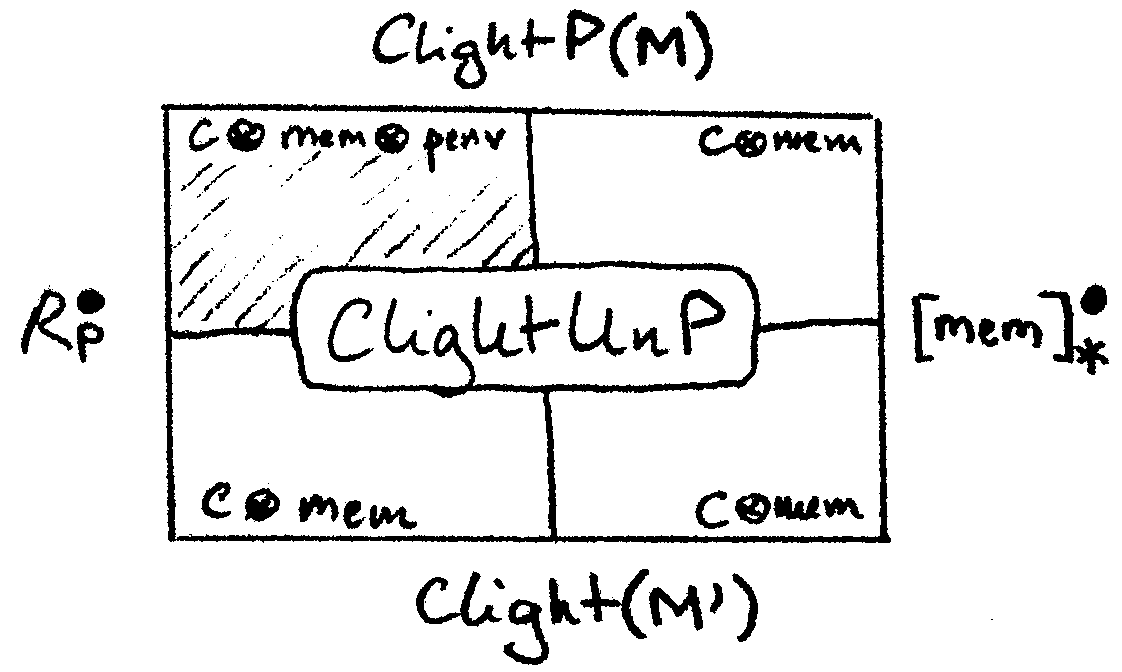
\includegraphics[scale=0.12]{draftfig/unclight}} }
  \qquad
  \text{where}
  \qquad
  \mathbf{R}_A :=
    \vcenter{ \hbox{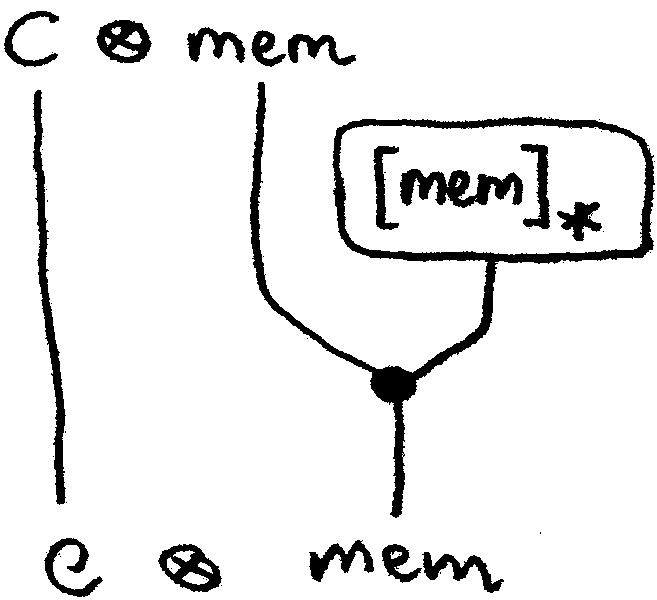
\includegraphics[scale=0.1]{draftfig/unclight-cca}} }
    \,,
  \qquad
  \mathbf{R}_B :=
    \vcenter{ \hbox{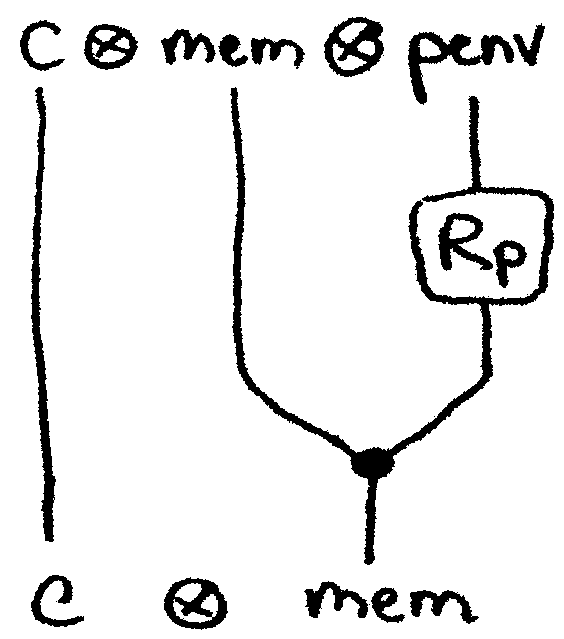
\includegraphics[scale=0.1]{draftfig/unclight-ccb}} }
    \,.
\]
In the Clight program,
formerly private variables are stored in the memory.
For incoming calls ($\mathbf{R}_B$),
we proceed as before and refine the private environment
into a memory share which is then merge with the main memory.
However, unlike layer interfaces,
ClightP program can also perform outgoing calls.
The use of
$\kw{r}_\kw{mem} : \mathbf{I} \Leftrightarrow \kw{mem}$
allows the target program to adjoin an extra memory share
for private variables
and requires the callee to leave this share unchanged.

Using ClightP,
implementing abstract data is a simple matter of
defining a relation $R \subseteq D \times \kw{penv}$.
We can then rely on $\kw{ClightUnP}$
to incorporate this abstract data into the global memory.

\begin{example}
Maybe the implementation of $L_\kw{rb}$?
\end{example}

%}}}

\subsection{Encapsulated State} %{{{

%In fact,
%multiple instances of $L$ may even be executing at the time
%if a reentrant call happens.
%Their internal states remain independent.
For the most part, the C language relies on a global memory state.
Because all components can in principle access every part of this global memory,
cross-component interactions carry the current state of the memory
back and forth with every question and answer.
Since C does not offer objects, closures or similar abstractions,
component-local state has a lifetime limited to a particular function activation.
In the semantics of CompCert languages,
maintaining persistent state across successive activations of a given component
would serve no purpose.

%Nevertheless, in many applications,
%the ability for a component to maintain local private state
%is important:
%\begin{itemize}
%  \item Beyond the world of C,
%    many language features behave in this way.
%    It is important to understand how CompCertO's approach
%    carries over to this context.
%  \item For verification,
%    we want make it a structural thing
%    rather than a rely/guarantee property we carry around everywhere.
%    Example: certified abstraction layers.
%\end{itemize}
%In the remainder of this section,
%we show how persistent, encapsulated state
%can be incorporated into
%the semantic model of CompCertO.

%}}}



%}}}

\section{A Double Category of Transition Systems} \label{sec:base} %{{{

% Preamble {{{

We begin our exposition by revisiting
the semantic model used in CompCertO.
As it stands (\S\ref{sec:basic:compcerto}),
this model offers only a very specific notion
of transition system composition,
meant to model program linking
in a context where
mutually recursive calls are possible.

By introducing a more general notion of composition (\S\ref{sec:basic:lcomp}),
we equip the model with the structure of a category.
This compositional structure
is preserved by an interpretation of CompCertO transition systems
into \emph{coherence spaces},
modeled after Reddy's object-based semantics (\S\ref{sec:basic:coh}).

In addition to transition systems,
CompCertO introduces a notion of \emph{simulation convention},
which formalizes the correspondance between the external interactions
of source- and target-level transition systems.
Simulation conventions carry their own categorical structure,
and together with transition systems and simulations
they constitute
a \emph{double category} $\mathbf{LTS}$ (\S\ref{sec:basic:double}).

This structure gives a formal underpinning to the usual notions of
horizontal and vertical composition
found in existing work on compositional certified compilers.
This richer structure
does not find a straightforward analogue
at the level of coherence spaces.
This illustrates an under-appreciated but important challenge
for denotational semantics in the context certified compilation,
namely the important role of abstraction
in that application domain.

%}}}

\subsection{Semantics in CompCertO} \label{sec:basic:compcerto} %{{{

As in the original CompCert semantics,
a transition system
executes by updating an internal state,
which is not directly observable
in its interactions with the environment.

\begin{definition} \label{def:lts} %{{{
A \emph{transition system} $L : A \twoheadrightarrow B$
is a tuple $L = \langle S, {\rightarrow}, I, X, Y, F \rangle$
consisting of:
\begin{itemize}
  \item a set $S$ of states;
  \item a transition relation ${\rightarrow} \subseteq S \times S$;
  \item a relation $I \subseteq B^\que \times S$
    which assigns possible \emph{initial states}
    to each question of $B$;
  \item a relation $F \subseteq S \times B^\ans$
    which specifies \emph{final states} together with
    corresponding answers in $B$;
  \item a relation $X \subseteq S \times A^\que$
    which identifies \emph{external states} and
    corresponding questions of $A$;
  \item a relation $Y \subseteq S \times A^\ans \times S$,
    which identifies \emph{resumption states}.
\end{itemize}
\end{definition}
%}}}

We use infix notation for the binary relations $I$, $F$, $X$.
We also write $r \mathrel{Y^s} s'$ when $(s, r, s') \in Y$;
this means that
after an external state $s$ triggers a question in $A^\que$ % ($s \mathrel{X} m$),
and the environment replies with an answer $r \in A^\ans$,
the execution resumes with state $s'$.
Hence,
when $L : A \twoheadrightarrow B$
performs an external call in $A$,
the internal state $s$ is preserved
until an answer resumes the execution.
Note that by contrast, in $B$
no state is preserved across invocations of $L$.
Each new question $q \in B^\que$ initializes a fresh state $s$
such that $q \mathrel{I} s$,
independently of any previous calls. % made into $L$.

\begin{example}[Clight semantics] \label{ex:clightsem} %{{{
[XXX update to refer to previous verion]

In CompCertO,
the semantics of a C translation unit $M$
is given as a transition system of type:
\[
  \kw{Clight}(M) : \mathcal{C}_\kw{m} \twoheadrightarrow \mathcal{C}_\kw{m}
\]
%Note that both incoming and outgoing call
%use the same language interface $\mathcal{C}_\kw{m}$.
%
Consider the translation unit $\kw{rb.c}$ shown in Fig.~\ref{fig:code}.
If $\kw{inc1}()$ is invoked
with a memory state where the variable $\kw{c1}$ has value $5$,
the transition system $\kw{Clight}(\kw{rb.c})$ will behave as follows:
\[
  \kw{inc1}()@m[\kw{c1} \mapsto 5]
  \mathrel{I}
  s_0 \rightarrow \cdots \rightarrow s_k
  \mathrel{F}
  5@m[\kw{c1} \mapsto 6]
\]
Note that the memory is updated to store the new value of the counter $\kw{c1}$.
By contrast, the function $\kw{deq}$ in $\kw{bq.c}$
does not directly modify the memory itself,
but it makes calls into $\kw{rb.c}$ which may have this effect.
The corresponding executions of $\kw{Clight}(\kw{bq.c})$
will have the shape
\begin{align*}
  \kw{deq}()@m
  \mathrel{I}
  u_0 \rightarrow \cdots \rightarrow u_1
  \mathrel{X}
  \kw{inc1}()@m &\leadsto i@m'
  \mathrel{Y^{u_1}}
  u_2 \rightarrow \cdots \\ \cdots \rightarrow u_3
  \mathrel{X}
  \kw{get}(i)@m' &\leadsto v@m''
  \mathrel{Y^{u_3}}
  u_4 \rightarrow \cdots \rightarrow u_5
  \mathrel{F}
  v@m''
  \,.
\end{align*}
\end{example}
%}}}

\subsubsection{Kripke Relators} %{{{

Logical relations
and relational parametricity
play an important role
in the construction of CompCertO's correctness theorem.
To state relational properties,
\citet{compcerto}
introduces a Kripke relator framework,
which we summarize below.
%We will use it
%to formulate various notions of simulation,
%and summarize it below.

Given two relations
$R \subseteq A \times B$ and
$S \subseteq U \times V$,
the relation
$(R \rightarrow S) \subseteq
 (A \rightarrow U) \times
 (B \rightarrow V)$
is defined in the usual way:
\[
  f \ifr{R \rightarrow S} g
  \quad:\Leftrightarrow\quad
  \forall (a, b) \in A \times B \mathbin.
    a \mathrel{R} b \Rightarrow
    f(a) \mathrel{S} g(b)
  \,.
\]
The more unusual powerset relator $\mathcal{P}^\le$
is used to express simulation diagrams.
Given $R \subseteq A \times B$,
the relation
$\mathcal{P}^\le(R) \subseteq \mathcal{P}(A) \times \mathcal{P}(B)$
is defined as:
\[
  x \ifr{\mathcal{P}(R)^\le} y
  \quad:\Leftrightarrow\quad
  \forall a \in x \mathbin.
  \exists b \in y \mathbin.
  a \mathrel{R} b
\]
To see how this works,
consider the simple transition systems
$\alpha : A \rightarrow \mathcal{P}(A)$
and
$\beta : B \rightarrow \mathcal{P}(B)$.
The relation $R$ is a simulation relation between them
when the following property holds:
\[
  \alpha \:\ifr{R \rightarrow \mathcal{P}^\le(R)}\: \beta
  \qquad\qquad\qquad
  \begin{tikzcd}
    a \ar[r, "\alpha"] \ar[d, dash, "R"'] &
    a' \ar[d, dash, dashed, "R"] \\
    b \ar[r, dashed, "\beta"'] &
    b'
  \end{tikzcd}
\]

Components of complex data structures
must often be related in ways which vary
depending on the context in which they appear,
or the history of the computation.
In such cases,
component relations can be indexed over a set of \emph{worlds},
which capture the relevant contextual information.
Formally, a \emph{Kripke relation} over a set of worlds $W$
is a ternary relation $R \subseteq W \times A \times B$.
We will write $R \in \mathcal{R}_W(A, B)$,
and use the notation
$
  w \Vdash a \mathrel{R} b
$
to mean that $(w, a, b) \in R$.
In addition,
\[
  {} \Vdash a \mathrel{R} b
  \quad :\Leftrightarrow \quad
  \forall w\in W \mathbin. w \Vdash a \mathrel{R} b
\]

It is often useful to let the world evolve
by endowing $W$ with an \emph{accessibility} relation
${\leadsto} \subseteq W \times W$.
World transitions are captured by the modal relator $\Diamond$,
which associates to a Kripke relation $R \in \mathcal{R}_W(A, B)$
the Kripke relation $\Diamond R$ of the same type, defined by:
\[
  w \Vdash a \ifr{\Diamond R} b
  \quad:\Leftrightarrow\quad
  \exists w' \mathbin. w \leadsto w' \wedge w' \Vdash a \mathrel{R} b
\]
For example,
a Kripke simulation between $\alpha : A \rightarrow \mathcal{P}(A)$
and $\beta : B \rightarrow \mathcal{P}(B)$
operating in the context of a Kripke frame $\langle W, {\leadsto} \rangle$
and a Kripke simulation relation $R \in \mathcal{R}_W(A, B)$
can be formulated in the following way.
The relators $\rightarrow$ and $\mathcal{P}^\le$
can be promoted to Kripke relators
by pointwise extension over the set of worlds.
The complex Kripke simulation property:
{\small
\[
  \forall w \in W \mathbin.
  \forall a \in A \mathbin.
  \forall b \in B \mathbin.
  w \Vdash a \mathrel{R} b \Rightarrow
  \forall a' \in \alpha(a) \mathbin.
  \exists b' \in \beta(b) \mathbin.
  \exists w' \in W \mathbin.
  w \leadsto w' \wedge w' \Vdash a' \mathrel{R} b'
\]
}
can be stated simply as:
\[
  \Vdash \alpha \ifr{R \rightarrow \mathcal{P}^\le(\Diamond R)} \beta
  \,.
\]

%}}}

\subsubsection{Simulations} %{{{

\begin{remark}[to incorporate]
In particular,
in the absence of demonic nondeterminism,
CompCert's notion of \emph{forward simulation} is appropriate:
given two transition systems $L_1$ and $L_2$,
it suffices to exhibit a relation between their possible states
such that:
\begin{itemize}
  \item initial state of $L_1$ have related initial states in $L_2$;
  \item state transitions in $L_1$ have corresponding sequences of transitions
    from related states in $L_2$;
  \item related state which produce a final outcome in $L_1$
    have a corresponding final outcome in $L_2$.
\end{itemize}
To take into account event traces,
the simulation works under the assumption that
$L_1$ and $L_2$ are fed the same inputs by the environement,
and requires that they produce identical outputs.
The existence of a simulation relation satisfying these properties
shows that the behavior of $L_1$ is refined by that of $L_2$;
we say that $L_1$ is simulated by $L_2$ and write $L_1 \le L_2$.
\end{remark}

The conventions $\mathbb{R}_A$ and $\mathbb{R}_B$
specify Kripke relations between source- and target-level interactions;
the Kripke worlds can be used to ensure that
question and their corresponding answers
are related in a consistent way.

\begin{definition}[Simulation Convention] \label{def:simconv}
Given two language interfaces $A$ and $B$,
a \emph{simulation convention} $\mathbb{R} : A \Leftrightarrow B$
is a set of worlds $W$ together with two relations:
\[
  \mathbb{R}^\que \in \mathcal{R}_W(A^\que, B^\que)
  \qquad
  \mathbb{R}^\ans \in \mathcal{R}_W(A^\ans, B^\ans)
\]
\end{definition}

Note that while simulation conventions
carry a set of worlds,
they do not specify an accessibility relation.

\begin{definition}[Basic Simulation] \label{def:sim}
\end{definition}

\begin{definition}[Composition of Simulation Conventions] \label{def:ccomp}
\end{definition}

\begin{theorem}[Vertical Composition] \label{thm:vcomp}
\end{theorem}

%}}}

%}}}

\subsection{Layered Composition} \label{sec:basic:lcomp} %{{{

To model linking,
CompCertO introduces an operator $\oplus$
which lets transition systems interact
by having them handle each other's external calls.
Because this operator permits mutual recursion,
it is limited to transition systems which perform
their incoming and outgoing calls
according to the same language interface:
\[
  {\oplus_A} :
    (A \twoheadrightarrow A) \times
    (A \twoheadrightarrow A) \rightarrow
    (A \twoheadrightarrow A)
\]
When mutual recursion is not needed,
we can instead use the operator
\[
  {\odot_{A,B,C}} :
    (B \twoheadrightarrow C) \times
    (A \twoheadrightarrow B) \rightarrow
    (A \twoheadrightarrow C)
  \,,
\]
which is simpler in its construction
and handles more general types.

%which reflects at the level of transition systems
%the categorical structure of $\ISpec$.

\begin{definition}[Composition of transition systems] \label{def:lcomp} %{{{
Suppose we have the transition systems
\[
  L_1 = \langle S_1, {\rightarrow_1}, I_1, X_1, Y_1, T_1 \rangle
    : B \twoheadrightarrow C
  \quad \text{and} \quad
  L_2 = \langle S_2, {\rightarrow_2}, I_2, X_2, Y_2, T_2 \rangle
    : A \twoheadrightarrow B
  \,.
\]
Their composition is defined as the transition system
$
  L_1 \odot L_2 :=
  \langle S, {\rightarrow}, I, X, Y, F \rangle
  : A \twoheadrightarrow C
$
with the following components.
States are taken in the set
$
    S := S_1 + (S_2 \times S_1)
$.
The left summand is used when $L_1$ is active.
The right summand is used when $L_2$ is active,
and keeps track of the suspended state of $L_1$
as well as the current state of $L_2$.
Initially, a call in $C$ activates $L_1$:
\[
  \begin{prooftree}
    \hypo{q_C \mathrel{I_1} s_1}
    \infer1{q_C \mathrel{I} \iota_1(s_1)}
  \end{prooftree}
  \qquad
  \begin{prooftree}
    \hypo{s_1 \rightarrow_1 s_1'}
    \infer1{\iota_1(s_1) \rightarrow \iota_1(s_1')}
  \end{prooftree}
  \qquad
  \begin{prooftree}
    \hypo{s_1 \mathrel{F_1} r_C}
    \infer1{\iota_1(s_1) \mathrel{F} r_C}
  \end{prooftree}
\]
When $L_1$ performs an external call in $B$,
its current state is saved and
the question activates $L_2$.
The execution proceeds
by updating the current $L_2$ state
and leaves the suspended state of $L_1$ untouched:
\[
  \begin{prooftree}
    \hypo{s_1 \mathrel{X_1} q_B}
    \hypo{q_B \mathrel{I_2} s_2}
    \infer2{\iota_1(s_1) \rightarrow \iota_2(s_2, s_1)}
  \end{prooftree}
  \qquad
  \begin{prooftree}
    \hypo{s_2 \rightarrow_2 s_2'}
    \infer1{\iota_2(s_2, s_1) \rightarrow \iota_2(s_2', s_1)}
  \end{prooftree}
  \qquad
  \begin{prooftree}
    \hypo{s_2 \mathrel{X_2} q_A}
    \infer1{\iota_2(s_2, s_1) \mathrel{X} q_A}
  \end{prooftree}
  \qquad
  \begin{prooftree}
    \hypo{r_A \mathrel{Y_2^{s_2}} s_2'}
    \infer1{r_A \mathrel{Y^{\iota_2(s_2, s_1)}} \iota_2(s_2', s_1)}
  \end{prooftree}
\]
When a final state of $L_2$ is reached,
$L_1$ is resumed:
\[
  \begin{prooftree}
    \hypo{s_2 \mathrel{F_2} r_B}
    \hypo{r_B \mathrel{Y_1^{s_1}} s_1'}
    \infer2{\iota_2(s_2, s_1) \rightarrow \iota_1(s_1')}
  \end{prooftree}
  \,.
\]
\end{definition}
%}}}

\begin{example}
Referring back to Example~\ref{ex:clightsem},
consider the transition system:
\[
  \kw{Clight}(\kw{bq.c}) \odot \kw{Clight}(\kw{rb.c}) :
  \mathcal{C}@\kw{mem} \twoheadrightarrow \mathcal{C}@\kw{mem}
  \,.
\]
There,
the calls of $\kw{bq.c}$ into $\kw{rb.c}$
are turned into internal steps,
triggering a switch between executions of the two components.
For example,
the call to $\kw{inc1}$ from $\kw{deq}$
may proceed as follows:
\begin{align*}
  \kw{deq}()@m[\kw{c_1} \mapsto 5] \mathrel{I} \iota_1(u_0)
  \rightarrow \cdots &\rightarrow \iota_1(u_1)
  \rightarrow \iota_2(s_0, u_1)
  \rightarrow \cdots \\ &\rightarrow \iota_2(s_k, u_1)
  \rightarrow \iota_1(u_2) \rightarrow \cdots
  \rightarrow \iota_1(u_5) \mathrel{F} v@m[\kw{c1} \mapsto 6]
\end{align*}
\end{example}

Like the symmetric composition operator $\oplus$ used in CompCertO,
the layered composition operator defined above
is compatible with simulations.

\begin{theorem}[Layered composition of simulations] \label{thm:lcompsim}
Simulations compose as follows:
\[
  \begin{prooftree}
    \hypo{L_1^\sharp
          \le_{\mathbb{R}_B \twoheadrightarrow \mathbb{R}_C}
          L_1^\flat}
    \hypo{L_2^\sharp
          \le_{\mathbb{R}_A \twoheadrightarrow \mathbb{R}_B}
          L_2^\flat}
    \infer2{L_1^\sharp \odot L_2^\sharp
          \le_{\mathbb{R}_A \twoheadrightarrow \mathbb{R}_C}
          L_1^\flat \odot L_2^\flat}
  \end{prooftree}
  \qquad \qquad
  \begin{tikzcd}
    A^\sharp \ar[r, twoheadrightarrow, "L_2^\sharp"]
             \ar[d, Leftrightarrow, "\mathbb{R}_A"'] &
    B^\sharp \ar[r, twoheadrightarrow, "L_1^\sharp"]
             \ar[d, Leftrightarrow, "\mathbb{R}_B"] &
    C^\sharp \ar[d, Leftrightarrow, "\mathbb{R}_C"]
    \\
    A^\flat \ar[r, twoheadrightarrow, "L_2^\flat"'] &
    B^\flat \ar[r, twoheadrightarrow, "L_1^\flat"'] &
    C^\flat
  \end{tikzcd}
\]
\end{theorem}

Importantly,
the composition operator $\odot$
\emph{under-approximates}
the semantic linking operator $\oplus$.
Since CompCert's syntactic linking of assembly programs
is known to implement $\oplus$,
this shows that linking is also a correct implementation of
the layered composition $\odot$.

\begin{theorem}[Linking implements layered composition]
For $L_1, L_2 : A \twoheadrightarrow A$,
\[
  L_1 \odot_{A,A,A} L_2
  \le
  L_1 \oplus_A L_2
 \,.
\]
\end{theorem}

%}}}

\subsection{Trace Semantics} \label{sec:basic:coh} %{{{

%}}}

\subsection{Double Category} \label{sec:basic:double} %{{{

%}}}

%}}}

\section{Explicit State} %{{{

We have mentioned in \S\ref{sec:basic:compcerto}
CompCertO's approach to \emph{state}:
the internal states of transition systems
cannot be observed across components and
persist only for the duration of a function activation;
therefore,
every question and answer must be annotated with
the current state of the global memory
at the time of a function's invocation or return,
as shown in the language interface $\mathcal{C}@\kw{mem}$
discussed in Example~\ref{ex:langint}.

In this section,
we show how this overall approach to persistent state
can be generalized,
and we introduce constructions
which can be used to manage
this kind of global state.

\subsection{Adjoining Explicit State} \label{sec:basic:state} %{{{

%In our approach to encapsulated state,
%we need to systematically
%annotate every question and answer
%in an existing language interface
%with a ``latest state'' field.
%The following constructions help us manage
%this kind of explicit state.

In Example~\ref{ex:langint} we gave a direct definition
for the language interface $\mathcal{C}@\kw{mem}$.
In fact,
this language interface can be derived from $\mathcal{C}$
by using the following operation.

\begin{definition}[Adjoining state]
Given a language interface $A = \langle A^\que, A^\ans \rangle$
and a set $K$,
the language interface $A@K$ is defined as:
\[
  A@K := \langle A^\que \times K ,\: A^\ans \times K \rangle
\]
We write the questions and answers of this language interface as
$q@k \in A^\que \times K$ and
$r@k \in A^\ans \times K$.
\end{definition}

Note that in our examples,
we have decomposed the CompCertO language interfaces
into $\mathcal{C}@\kw{mem}$, $\mathcal{A}@\kw{mem}$, etc.
The memory state is dropped from the language interface $\mathcal{C}$,
whose questions are now just $f[\mathit{sg}](\vec{v})$,
and reintroduced with $@\kw{mem}$ to obtain
the full question $f[\mathit{sg}](\vec{v})@m$.
This will be used in the context of CAL
where layer interfaces can be defined in a memory-free manner
($\mathcal{C}$ without $@\kw{mem}$),
their behavior being entirely determined by their encapsulated state.

\begin{example}[Layer specifications] \label{ex:rbspec} %{{{
We can formulate a specification for
the program component $\kw{rb.c}$ as follows.
The state of the ring buffer
is expressed as a tuple
$(f, c_1, c_2) \in S_\kw{rb} := \kw{val}^N \times \mathbb{N} \times \mathbb{N}$.
Operations do not otherwise access the memory,
so the specification will be of type
\[
  L_\kw{rb} : \mathbf{1} \twoheadrightarrow \mathcal{C}@S_\kw{rb}
  \,.
\]
To define it, we construct a simple transition system such that
all executions take the shape
\[
  q@(f, c_1, c_2) \:\mathrel{I}\: (v', f', c_1', c_2')
                  \:\mathrel{F}\: v'@(f', c_1', c_2')
  \,.
\]
The predicates $X$, $Y$ and $\rightarrow$ are empty.
As suggested above, $F$ is in essence the identity relation.
This leaves us to define $I$ which specifies the component's
actual behavior:
\[ \begin{array}{c@{\qquad}c}
 {\begin{prooftree}
    \hypo{i < N}
    \infer1{
      \kw{set}(i, v)@(f, c_1, c_2)
      \mathrel{I_\kw{rb}}
      (\kw{undef}, f[i := v], c_1, c_2)}
  \end{prooftree}}
  &
 {\begin{prooftree}
    \hypo{c_1' = (c_1 + 1) \mathbin{\mathrm{mod}} N}
    \infer1{
      \kw{inc1}@(f, c_1, c_2)
      \mathrel{I_\kw{rb}}
      (c_1, f, c_1', c_2)}
  \end{prooftree}}
  \vspace{1em}
  \\
 {\begin{prooftree}
    \hypo{i < N}
    \infer1{
      \kw{get}(i)@(f, c_1, c_2)
      \mathrel{I_\kw{rb}}
      (f_i, f, c_1, c_2)
    }
  \end{prooftree}}
  &
 {\begin{prooftree}
    \hypo{c_2' = (c_2 + 1) \mathbin{\mathrm{mod}} N}
    \infer1{
      \kw{inc1}@(f, c_1, c_2)
      \mathrel{I_\kw{rb}}
      (c_2, f, c_1, c_2')}
  \end{prooftree}}
\end{array} \]
We can then define
$L_\kw{rb} := \langle
  S_\kw{rb},\:
  \varnothing,\:
  I_\kw{rb},\:
  \varnothing,\:
  \varnothing,\:
  {=}
 \rangle$.

A similar approach can be use to define
$L_\kw{bq} : \mathbf{1} \twoheadrightarrow \mathcal{C}@S_\kw{bq}$,
where the states in $S_\kw{bq} := \kw{val}^*$
are simply lists enumerating the contents of the queue.
Here the operations will be specified as follows:
\[
  \begin{prooftree}
    \hypo{|\vec{q}| < N}
    \infer1{\kw{enq}(v)@\vec{q} \:\mathrel{I_\kw{bq}}\: (\kw{undef}, \vec{q}v)}
  \end{prooftree}
  \qquad\qquad
  \begin{prooftree}
    \hypo{\vec{q} = v\vec{p}}
    \infer1{\kw{deq}(\epsilon)@\vec{q} \:\mathrel{I_\kw{bq}}\: (v, \vec{p})}
  \end{prooftree}
\]
Again we can define $L_\kw{bq} := \langle
  S_\kw{bq},\:
  \varnothing,\:
  I_\kw{bq},\:
  \varnothing,\:
  \varnothing,\:
  {=}
\rangle$.
\end{example}
%}}}

Often,
we will want to add a state annotation
to the interface of an existing component.
When lifting $L : A \twoheadrightarrow B$
to operate as $L@K : A@K \twoheadrightarrow B@K$,
the resulting transition system
remains insensitive to the state annotation $K$,
but keeps track of its value
across all of its interactions.

\begin{definition}[Lifting] \label{def:lift} %{{{
Given %the transition system
$L = \langle S, {\rightarrow}, I, X, Y, F \rangle : A \twoheadrightarrow B$
we define $L@K : A@K \twoheadrightarrow B@K$ as:
\begin{gather*}
  L@K := \langle S \times K, {\rightarrow_K}, I_K, X_K, Y_K, F_K \rangle \\
 {\begin{prooftree}
    \hypo{q \mathrel{I} s}
    \infer1{q@k \mathrel{I_K} s@k}
  \end{prooftree}}
  \qquad
 {\begin{prooftree}
    \hypo{s \rightarrow s'}
    \infer1{s@k \rightarrow_K s'@k}
  \end{prooftree}}
  \qquad
 {\begin{prooftree}
    \hypo{s \mathrel{X} m}
    \infer1{s@k \mathrel{X_K} m@k}
  \end{prooftree}}
  \qquad
 {\begin{prooftree}
    \hypo{n \mathrel{Y}^s s'}
    \infer1{n@k' \mathrel{Y^{s@k}_K} s'@k'}
  \end{prooftree}}
  \qquad
 {\begin{prooftree}
    \hypo{s \mathrel{F} r}
    \infer1{s@k \mathrel{F_K} r@k}
  \end{prooftree}}
\end{gather*}
\end{definition}
%}}}

This construction is used in particular when components are linked,
to pass through the internal state of other components.

\begin{example}[Interfacing $L_\kw{rb}$ with client code] \label{ex:context}
Building on Example~\ref{ex:rbspec},
consider the problem of interfacing
the client code in $\kw{bq.c}$ with the underlay interface $L_\kw{rb}$.
The types
\[
  L_\kw{rb} : \mathbf{1} \twoheadrightarrow \mathcal{C}@S_\kw{rb}
  \qquad
  \text{and}
  \qquad
  \Clight(\kw{bq.c}) : \mathcal{C}@\kw{mem} \twoheadrightarrow \mathcal{C}@\kw{mem}
\]
are not directly compatible,
given that $L_\kw{rb}$ manipulates a state of type $S_\kw{rb}$
and $\kw{rb.c}$ expects a memory state of type $\kw{mem}$.
The solution is to lift each one to ``pass through''
the state of the other:
\[
  \begin{tikzcd}[column sep=huge]
    \mathbf{1}@\kw{mem}
    \ar[r, "L_\kw{rb}@\kw{mem}"] &
    \mathcal{C}@S_\kw{rb}@\kw{mem} \cong
    \mathcal{C}@\kw{mem}@S_\kw{rb}
    \ar[r, "\Clight(\kw{bq.c})@S_\kw{rb}"] &
    \mathcal{C}@\kw{mem}@S_\kw{rb}
  \end{tikzcd}
\]
Implicitly taking into account the isomorphisms
\[
  \mathbf{1} \cong \mathbf{1}@\kw{mem}
  \qquad
  \text{and}
  \qquad
  \mathcal{C}@S_\kw{rb}@\kw{mem} \cong
  \mathcal{C}@\kw{mem}@S_\kw{rb} \cong
  \mathcal{C}@(S_\kw{rb} \times \kw{mem})
  \,,
\]
they can then be composed into
\begin{gather*}
  \Clight(\kw{bq.c})@S_\kw{rb} \odot
  L_\kw{rb}@\kw{mem} :
  \mathbf{1} \twoheadrightarrow \mathcal{C}@(S_\kw{rb} \times \kw{mem})
  \,.
\end{gather*}

To establish that this combination implements the overlay interface $L_\kw{bq}$,
we can lift the latter to:
\[
  L_\kw{bq}@\kw{mem} : \mathbf{1} \twoheadrightarrow
    \mathcal{C}@(S_\kw{bq} \times \kw{mem})
  \,.
\]
We will then need to define a simulation convention
explaining the relationship between
the states of type $S_\kw{bq}$ used by the specification and
the states of type $S_\kw{rb}$ used by the implementation.

%}}}

\subsection{Certified Abstraction Layers} \label{sec:basic:abrel} %{{{

In Example~\ref{ex:context},
because of the difference between
the abstract state components $S_\kw{rb}$ and $S_\kw{bq}$,
they cannot be compared directly.
We must first explain the correspondence between
the two types of abstract states
by formulating a proper simulation convention.
This can be done as follows.
\end{example}

\begin{definition}
For a language interface $A$ and a relation $R \subseteq K_1 \times K_2$,
we define the simulation convention $A@R : A@K_1 \Leftrightarrow A@K_2$ as
$
  A@R := \langle \mathbf{1}, \: {=} \times R, \: {=} \times R \rangle
$.
\end{definition}

The simulation convention $A@R$
can be used to relate transition systems which use
different types of explicit state.
The \emph{abstraction relation} $R$
specifies the correspondence between the two.

\begin{example}[Correctness of \kw{bq.c}] \label{ex:bqcorrect}
Carrying on with our running example,
using the abstraction relation $R \subseteq S_\kw{bq} \times S_\kw{rb}$
given in \citet{rbgs-cal}:
\begin{align*}
  \vec{q} \mathrel{R} (f, c_1, c_2) \:\Leftrightarrow\: {}
    & (c_1 \le c_2 < N \:\wedge\: \vec{q} = f_{c_1} \cdots f_{c_2-1}) \vee {} \\
    & (c_2 \le c_1 < N \:\wedge\: \vec{q} = f_{c_1} \cdots f_{N-1} f_0 \cdots f_{c_2 - 1})
\end{align*}
we can formulate the correctness criterion:
\[
  L_\kw{bq}@\kw{mem}
  \:\le_{\kw{id} \twoheadrightarrow \mathcal{C}@({=}_\kw{mem} \times R)}\:
  \Clight(\kw{bq.c})@S_\kw{rb} \odot
  L_\kw{rb}@\kw{mem}
  \,.
\]
\end{example}

This approach also works in more complex situations.
For example,
if part of a layer's abstract state is
stored in the memory by its implementation,
or if the implementation uses additional memory blocks
for its own purposes,
the abstraction relation ${=}_\kw{mem} \times R$
can be transformed to reflect those details.
This makes it possible for CompCertO
to support certified abstraction layers.

However,
in the framework outlined so far,
the user is expected to manage state explicitly.
Ideally,
once a layer has been implemented,
these details could be hidden so that
high-level composition and reasoning
in which they play no role
can be carried out without any unnecessary
encumbrance.
The next section
extends our framework
with state encapsulation primitives
to make this possible.

%In our treatment of certified abstraction layers (\S\ref{sec:cal}),
%we will use this construction as well
%to lift a memory-free layer interface $\Sigma : \mathbf{1} \rightarrow \mathcal{C}$
%to $\Sigma@\kw{mem} : 1 \rightarrow \mathcal{C}@\kw{mem}$,
%making it possible to interface it with client code.

%}}}

%}}}

\section{Encapsulated State} \label{sec:encap} %{{{

% Preamble {{{

As discussed in \S\ref{sec:basic:compcerto},
state in CompCertO exists in two forms:
\begin{itemize}
  \item The memory state is global and persistent.
    It is shared across all components
    and must be carried along
    every time a question or answer transfers control
    between components.
  \item States within transition systems
    are private to each component.
    They can only be observed indirectly,
    through a component's behavior
    in future interactions with its environment.
\end{itemize}
State of the first kind
is managed using language interfaces
of the form $A@K$.
Lifted components, of the form $L@K$,
are insensitive to the global state $k$
but pass it along unchanged
when activated.
The second kind of state is \emph{encapsulated}---%
local to a component
and inaccessible to the environment.
In CompCertO, the scope of encapsulated state
can only be a specific activation of the component.

In this section,
we explain how a richer model can be constructed
to allow encapsulated state
to be \emph{persistent} across
successive activations of a component.
Such persistent state
is communicated from one activation to the next
in the same way global state would be,
but is marked as local to a given component
to ensure that the environment cannot interfere
with it between successive activations.

%}}}

\subsection{Stateful Components} %{{{

Consider two transition systems $L_1$ and $L_2$
which interact as follows:
\[
  \begin{tikzcd}[row sep=small, column sep=large]
    & B \ar[r, twoheadrightarrow, "L_1"] & C \\
    A \ar[r, twoheadrightarrow, "L_2"] &
    B@K \ar[r, twoheadrightarrow, "L_1@K"] &
    C@K
  \end{tikzcd}
\]
The component $L_2$ expects
incoming questions and answers in $B$
to carry a persistent state $k \in K$.
With each question in $B$,
it may use this state to adjust its behavior.
With each answer,
it can communicate back an updated state to the caller.
By contrast,
$L_1@K$ is by construction insensitive to $k$,
which cannot influence the behavior of $L_1$
and is passed unchanged
between $L_2$ and the environment.

In other words,
from the point of view of $L_1$,
the state $k \in K$ is not directly observable.
If we require that any further components
added to the system
behave in the same way with respect to $K$,
in effect $k$ will become encapsulated state of $L_2$.
Based on this insight,
we define a stateful component as follows.

\begin{definition} \label{def:slts}
A stateful component
$\Sigma = (\intl{k} \in K \mid L) : A \rightarrow B$.
consists of:
\begin{itemize}
  \item a set of states $K$;
  \item an initial state $\intl{k} \in K$;
  \item a transition system $L : A \twoheadrightarrow B@K$.
\end{itemize}
\end{definition}

From $\Sigma$'s point of view,
the environment behaves in the following way.
The first time $\Sigma$ is activated by a question $q \in B^\que$,
the state $\intl{k}$ is adjoined to $q$
and the transition system $L$ is initialized using the question $q@\intl{k}$.
When $L$ terminates with an answer $r@k' \in (B@K)^\ans$,
the private state component $k'$
is set aside until
the next activation of $\Sigma$,
at which point it is fed back to $L$ and so on.

A CompCertO LTS $L : A \twoheadrightarrow B$
can be lifted to the persistent version
by using a unit state:
\[
  \begin{prooftree}
    \hypo{L : A \twoheadrightarrow B}
    \infer1{\&L := (\mathbbm{1} \mid L) : A \rightarrow B}
  \end{prooftree}
\]
State encapsulation is managed using an operation
\[
  \begin{prooftree}
    \hypo{\Sigma = (Q \mid L) : A \rightarrow B@K}
    \infer1{\mathsf{fbk}_K(\Sigma) := (Q \times K \mid L) : A \rightarrow B}
  \end{prooftree}
\]
which adds a field of type $K$ to the encapsulated state within $\Sigma$.

Once private state has been encapsulated,
in principle it can only be observed by the environment
through the way the transition system responds
to successive queries.
In particular,
constructions on stateful components
should preserve the following notion of equivalence.

\begin{definition}[Simple Simulation] \label{def:ssim}
We will say that $\Sigma_1 : A \rightarrow B$
is refined by $\Sigma_2 : A \rightarrow B$
and write $\Sigma_1 \preceq \Sigma_2$
when there exists a relation $R \subseteq K_1 \times K_2$
such that:
\begin{itemize}
  \item the initial states $\intl{k}_1, \intl{k}_2$ are related by $R$;
  \item the transition systems satisfy
    $L_1 \le_{\kw{id}_A \twoheadrightarrow B@R} L_2$.
\end{itemize}
We write $\Sigma_1 \equiv \Sigma_2$ when
$\Sigma_1 \preceq \Sigma_2$ and
$\Sigma_2 \preceq \Sigma_1$.
\end{definition}

%}}}

\subsection{Composition} %{{{

The composite $\Sigma_1 \circ \Sigma_2$
uses states of type $K_1 \times K_2$.
Each side of the pair is updated
when the corresponding component is active.
Incoming questions in $C$ are routed to $L_1 : B \twoheadrightarrow C@K_1$,
which we lift to pass through an additional state component of type $K_2$.
Outgoing questions of $L_1$ in $B$ can then be routed to $L_2$,
as depicted in the following diagram:
\[
  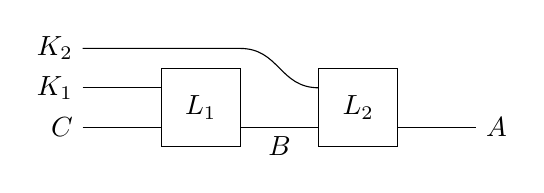
\begin{tikzpicture}[yscale=0.5]
    \draw (0,2) node[left] {$K_2$} -- (2,2) .. controls +(0.5,0) and +(-0.5,0) .. (3,1);
    \draw (0,1) node[left] {$K_1$} -- (1,1);
    \draw (0,0) node[left] {$C$} -- (1,0);
    \draw (2,0) -- node[below] {$B$} (3,0);
    \draw (4,0) -- (5,0) node[right] {$A$};
    \draw (1,1.5) rectangle node {$L_1$} (2,-0.5);
    \draw (3,1.5) rectangle node {$L_2$} (4,-0.5);
  \end{tikzpicture}
\]
Formally,
composition is defined as follows.

\begin{definition}[Composition] \label{def:slcomp}
Given two stateful components
$\Sigma_1 = (K_1 \mid L_1) : B \rightarrow C$ and
$\Sigma_2 = (K_2 \mid L_2) : A \rightarrow B$,
we define their composition
$\Sigma_1 \circ \Sigma_2 : A \rightarrow C$
in the following way:
\[
  \Sigma_1 \circ \Sigma_2 :=
    ( K_1 \times K_2 \mid L_1@K_2 \odot L_2 )
\]
Note that this formulation
implicitly uses the isomorphism
\[
  L_1@K_2 : B@K_2 \twoheadrightarrow (C@K_1)@K_2 \cong C@(K_1 \times K_2)
  \,.
\]
\end{definition}




\begin{lemma}
  This is compatible with:
  \begin{itemize}
    \item simple simulations;
    \item lifting hence associativity is preserved.
  \end{itemize}

\end{lemma}

%}}}

\subsection{Combining Hidden and Explicit State} %{{{

It is possible for a stateful component
to hide only part of the explicit state
used by the underlying transition system.
For example,
in a transition system
$L : A \rightarrow B@(K \times U) \cong B@U@K$,
we may choose to hide only $K$,
to obtain a stateful component
$\Sigma = (K \mid L) : A \rightarrow B@U$
which still exchanges explicit state of type $U$
with the environment.
This makes it possible to construct
complex stateful components incrementally
from simpler, stateless parts,
by first promoting them using $\&$,
then hiding state in a step-by-step fashion
using $\kw{fbk}$.

In addition,
stateful components can be lifted
to pass through explicit state.

\begin{definition} \label{def:slift}
The stateful component $\Sigma = (K \mid L) : A \rightarrow B$
can be lifted to \[ \Sigma@U := (K \mid L@U) : A@U \rightarrow B@U \,. \]
Note that this relies on the isomorphism
\[
  L@U : A@U \twoheadrightarrow (B@K)@U \cong (B@U)@K
  \,.
\]
\end{definition}

The following properties
relate the promotion operator $\&$,
the composition operators $\odot$ and $\circ$,
and the hiding operator $\kw{fbk}$.

\begin{lemma}
  For $L_1 : B \twoheadrightarrow C@K_1$ and
  $L_2 : A \twoheadrightarrow B@K_2$,
  the following property holds:
  \[
    \&(L_1@K_2) \circ \&L_2 \equiv \&(L_1@K_2 \odot L_2)
    \,.
  \]
  In addition, for $\Sigma_1 : B \rightarrow C@U_1$
  and $\Sigma_2 : A \rightarrow B@U_2$,
  the following property holds:
  \[
    \kw{fbk}_{U_1}(\Sigma_1) \circ \kw{fbk}_{U_2}(\Sigma_2) \equiv
    \kw{fbk}_{U_1 \times U_2}(\Sigma_1@U_2 \circ \Sigma_2)
    \,.
  \]
\end{lemma}

%}}}

\subsection{Stateful Simulations} %{{{

Definition XXX introduced a simple notion of refinement
between stateful components,
but assumed that the interactions of both components
with their environment were identical.
By contrast, a key feature of CompCertO
is the notion of \emph{simulation convention},
which parameterizes simulations by
specifying how the interactions of
the source-level and target-level transition system
are related.

\subsubsection{Stateful Simulation Conventions} %{{{

Transition systems in CompCertO are stateless,
and as a consequence,
successive activations of given
source- and target-level
transition systems can be related in the same way.
By contrast,
our components may maintain encapsulated states
and behave differently upon successive activations.
As a consequence,
the relationship between source- and target-level interactions
may depend on the history of the computation.
This means we must generalize simulation conventions
so that they may maintain their own state as well.

\begin{definition} \label{def:sconv} %{{{
A \emph{stateful simulation convention}
$\mathbf{R} = \langle W, {\leadsto}, {\mapsto}, R^\que, R^\ans \rangle$
between the language interfaces $A^\sharp$ and $A^\flat$
is specified by:
\begin{itemize}
  \item a pointed set of worlds $W$,
    which store the current state of the simulation convention;
  \item two accessibility relations
    ${\leadsto}, {\mapsto} \subseteq W \times W$,
    corresponding to \emph{internal} and \emph{external} transitions;
  \item a Kripke relation $R^\que \in \mathcal{R}_W(A_\sharp^\que, A_\flat^\que)$
    between the language interfaces' questions, and
  \item a Kripke relation $R^\ans \in \mathcal{R}_W(A_\sharp^\ans, B_\flat^\ans)$
    between their answers.
\end{itemize}
The accessibility relations are required to be reflexive and transitive.
We write $\mathbf{R} : A^\sharp \leftrightarrow A^\flat$.
The identity simulation convention
$\kw{id}_A : A \leftrightarrow A$
is given by
$\kw{id}_A := \langle
    \mathbbm{1}, {=}_\mathbbm{1}, {=}_\mathbbm{1}, {=}_{A^\que}, {=}_{A^\ans}
 \rangle$.
\end{definition}
%}}}

The initial world $\intl{w}$ gives the simulation convention's initial state.
While the environment is in control,
the world may transition according to the relation $\mapsto$.
When control is transferred to the system,
the corresponding questions must be related by $w \Vdash R^\que$.
World transitions may then occur according to $\leadsto$.
Hence, when the system returns control to the environment,
the corresponding answers
will be related by $w' \Vdash R^\ans$,
where $w'$ is a successor world of $w$ such that $w \leadsto w'$.
The questions for any subsequent activation
must in turn be related at a world $w''$ such that $w' \mapsto w''$,
and so on and so forth indefinitely:
\begin{align*}
  \intl{w} \mapsto w_1 &\Vdash q^\sharp_1 \mathrel{R^\que} q^\flat_1 \\
  w_1 \leadsto w_1' &\Vdash r^\sharp_1 \mathrel{R^\ans} r^\flat_1 \\
  w_1' \mapsto w_2 &\Vdash q^\sharp_2 \mathrel{R^\que} q^\flat_2 \\
  w_2 \leadsto w_2' &\Vdash r^\sharp_2 \mathrel{R^\ans} r^\flat_2 \\[-1ex]
  &\:\:\vdots
\end{align*}

%}}}

\subsubsection{Stateful Simulations of Transition Systems} %{{{

Before we define simulations between stateful components,
we first update CompCertO's notion of simulation of transition systems
to take into account stateful conventions.
%In particular,
%using stateful simulation conventions,
%the sequence of external calls performed by a transition system
%will become important.

Consider a simulation of type:
\[
\begin{tikzcd}
  A_1 \ar[r, twoheadrightarrow, "L_1"] \ar[d, leftrightarrow, "\mathbf{R}_A"'] &
  B_1 \ar[d, leftrightarrow, "\mathbf{R}_B"] \\
  A_2 \ar[r, twoheadrightarrow, "L_2"] & B_2
\end{tikzcd}
\]
The simulation simultaneously
plays the role of the system with respect to
the simulation convention $\mathbf{R}_B$ and
the role of the environment with respect to $\mathbf{R}_A$.
Hence,
it will operate in the context of a Kripke frame
constructed from both $W_A$ and $W_B$.
The possible states of a simulation will be a subset
$W \subseteq W_A \times W_B$,
which must contain
the initial state $\intl{w} := (\intl{w}_A, \intl{w}_B) \in W$.
Between successive activations,
the environment may update the $W_B$ component.
Hence we require:
\[
  (w_A, w_B) \in W \:\wedge\:
  w_B \mapsto_B w_B' \:\Rightarrow\:
  (w_A, w_B') \in W
\]
When the components execute,
the worlds will evolve according to
the accessibility relation:
\[
  (w_A, w_B) \leadsto_{\bar{A}B} (w_A', w_B') \::\Leftrightarrow\:
  w_A \mapsto_A w_A' \:\wedge\: w_B \leadsto_B w_B'
\]
Reading the constituent transition relations
within $L_1, L_2$ as functions of type:
\begin{align*}
  I_1 &: B_1^\que \rightarrow \mathcal{P}(S_1) &
  {\rightarrow_1} &: S_1 \rightarrow \mathcal{P}(\mathbb{E}^* \times S_1) &
  F_1 &: S_1 \rightarrow \mathcal{P}(B_1^\ans)
  \\
  I_2 &: B_2^\que \rightarrow \mathcal{P}(S_2) &
  {\rightarrow_2} &: S_2 \rightarrow \mathcal{P}(\mathbb{E}^* \times S_2) &
  F_2 &: S_2 \rightarrow \mathcal{P}(B_2^\ans)
  \,,
\end{align*}
we can formulate the simulation properties for internal steps
concisely as shown in Fig.~\ref{fig:simint}.
\begin{figure}[h]
  \small
  \[
    \begin{array}{c@{\qquad}c@{\qquad}c}
      \begin{tikzcd}[sep=tiny,column sep=0]
        q_1 \ar[dd, "w \Vdash \mathbf{R}_B^\que"', dash] \ar[rr, dash, "I_1"] &&
        s_1 \ar[dd, "w' \Vdash R", dash, dashed] \\
        & \leadsto_{\bar{A}B} & \\
        q_2 \ar[rr, "I_2"', dash, dashed] &&
        s_2
      \end{tikzcd}
      &
      \begin{tikzcd}[sep=tiny,column sep=0]
        s_1 \ar[rr, "t"] \ar[dd, "w \Vdash R"', dash] &&
        \!\!{}_1 \:\, s_1' \ar[dd, "w' \Vdash R", dash, dashed] \\
        & \leadsto_{\bar{A}B} & \\
        s_2 \ar[rr, "t", dashed] &&
        \!\!{}_2^* \:\, s_2'
      \end{tikzcd}
%      \begin{tikzcd}[sep=large]
%        s_1 \ar[r] \ar[d, "{(w_A, w_B) \Vdash R}"', dash] &
%        s_1' \ar[d, "{(w_A,w_B) \Vdash R}", dash, dashed] \\
%        s_2 \ar[r, dashed] &
%        \!\!\!{}^* \: s_2'
%      \end{tikzcd}
      &
      \begin{tikzcd}[sep=tiny, column sep=0]
        s_1 \ar[rr, "F_1", dash] \ar[dd, "w \Vdash R"', dash] &&
        r_1 \ar[dd, "w' \Vdash \mathbf{R}_B^\ans", dash, dashed] \\
        & \leadsto_{\bar{A}B} & \\
        s_2 \ar[rr, "F_2"', dash, dashed] &&
        r_2
      \end{tikzcd}
      \vspace{1ex} \\
      I_1 \ifr{\Vdash \mathbf{R}_B^\que \rightarrow
        \mathcal{P}^\le(\Diamond_{\bar{A}B} R)} I_2
      &
      {\rightarrow_1}
      \ifr{\Vdash R \rightarrow \mathcal{P}^\le(\Diamond_{\bar{A}B} ({=} \times R))}
      {\rightarrow_2^*}
      &
      F_1
      \ifr{\Vdash R \rightarrow \mathcal{P}^\le(\Diamond_{\bar{A}B} \mathbf{R}_B^\ans)}
      F_2
      \vspace{1.2ex} \\
      \text{(a) Initial states} &
      \text{(b) Internal states} &
      \text{(c) Final states}
    \end{array}
  \]
  \caption{Stateful simulation properties for internal steps}
  \label{fig:simint}
\end{figure}

Conversely, for external calls,
the simulation plays the role of the environment.
We expect that:
\[
  (w_A, w_B) \in W \:\wedge\:
  w_A \leadsto_A w_A' \:\Rightarrow\:
  (w_A', w_B) \in W
\]
Moreover,
from the point of view of the simulation,
an external call will make a transition according to
the following accessibility relation:
%[NB we may want to restrict $\leadsto_B$ to $=$
%if this causes problems, but]
%Note that by allowing a transition $w_B \leadsto_B w_B'$,
%we are able to capture the effect that
%any reentrant call may have on the simulation state:
\[
  (w_A, w_B) \leadsto_{AB} (w_A', w_B') \::\Leftrightarrow\:
  w_A \leadsto_A w_A' \:\wedge\:
  w_B = w_B'
\]
By reading the action of transition systems at external calls
in terms of the functions:
\begin{align*}
  Z_1 &: S_1 \rightarrow
    \mathcal{P}(A_1^\que \times (A_1^\ans \rightarrow \mathcal{P}(S_1))) &
  Z_1(s_1) &:= \{ (q_1, Y_1^{s_1}) \mid s_1 \mathrel{X_1} q_1 \}
 \\
  Z_2 &: S_2 \rightarrow
    \mathcal{P}(A_2^\que \times (A_2^\ans \rightarrow \mathcal{P}(S_2))) &
  Z_2(s_2) &:= \{ (q_2, Y_2^{s_2}) \mid s_2 \mathrel{X_2} q_2 \}
  \,,
\end{align*}
we can then formulate the simulation condition for external calls
as presented in Fig.~\ref{fig:simext} below.

\begin{figure}[h]
  \[
    \begin{array}{c}
      \begin{tikzcd}[sep=tiny, column sep=small]
        s_1 \ar[rr, "X_1", dash] \ar[dd, "w \Vdash R"', dash] &&
        m_1 \ar[rr, dotted, dash] \ar[dd, "w'"', "{} \Vdash \mathbf{R}_A^\que", dash, dashed] &&
        n_1 \ar[rr, "Y_1^{s_1}", dash] \ar[dd, "w''"', "{} \Vdash \mathbf{R}_A^\ans", dash] &&
        s_1' \ar[dd, "w''' \Vdash R", dash, dashed]
        \\
        & \leadsto_{\bar{A}B} && \leadsto_{AB} && \leadsto_{\bar{A}B} &
        \\
        s_2 \ar[rr, "X_2"', dash, dashed] &&
        m_2 \ar[rr, dotted, dash] &&
        n_2 \ar[rr, "Y_2^{s_2}"', dash, dashed] &&
        s_2'
      \end{tikzcd}
      \vspace{1ex} \\
      Z_1
      \mathrel{[
        \Vdash R \rightarrow \mathcal{P}^\le(
          \Diamond_{\bar{A}B} (
          \mathbf{R}_A^\que \times
            \Box_{AB} (
            \mathbf{R}_A^\ans \rightarrow
            \mathcal{P}^\le(\Diamond_{\bar{A}B} R))))
      ]}
      Z_2
    \end{array}
  \]
  \caption{Simulation property for external states}
  \label{fig:simext}
\end{figure}

\begin{definition}[Stateful simulation]
A stateful simulation of CompCertO transition systems,
written as
$L_1 \preceq_{\mathbf{R}_A \twoheadrightarrow \mathbf{R}_B} L_2$,
is given by a set of worlds $W$ such that
\[ (\intl{w}_A, \intl{w}_B) \in W \subseteq W_A \times W_B \,, \]
closed under ${\leadsto_A} \times {\mapsto_B}$,
satisfying the properties given in
\autoref{fig:simint} and
\autoref{fig:simext}.
\end{definition}

Note that the stateless simulation conventions of CompCertO
can be promoted as follows.

\begin{definition}[Promoted simulation convention]
The CompCertO simulation convention
$\mathbb{R} = \langle W, \mathbb{R}^\que, \mathbb{R}^\ans \rangle$
can be promoted to the stateful simulation convention
$\&\mathbb{R} :=
 \langle W_*, {=}, \top, \mathbb{R}^\que_*, \mathbb{R}^\ans_* \rangle$.
The pointed set $W_* = W \cup \{ \intl{*} \}$
introduces a new initial world $*$.
The relations $\mathbb{R}^\que_*$ and $\mathbb{R}^\ans_*$
are empty at this initial world,
but the environment can transition
to any world $w \in W$ (${\mapsto} := \top$).
The system must leave the world unchanged (${\leadsto} := {=}$).
\end{definition}

Then we have the relationship:
\begin{lemma}[CompCertO \emph{vs\@.} stateful simulations] \label{lemma:stsim}
\[
  L_1 \le_{\mathbb{R}_A \twoheadrightarrow \mathbb{R}_B} L_2
  \quad \Leftrightarrow \quad
  L_1 \preceq_{\&\mathbb{R}_A \twoheadrightarrow \&\mathbb{R}_B} L_2
\]
\end{lemma}

As with simulations in CompCertO,
stateful simulations compose both horizontally and vertically.
The horizontal (layered) composition of simulations
is as follows.

\begin{lemma}[Layered composition of stateful simulations]
\[
  \begin{prooftree}
    \hypo{
      L_1^\sharp
      \preceq_{\mathbf{R}_B \twoheadrightarrow \mathbf{R}_C}
      L_1^\flat}
    \hypo{
      L_2^\sharp
      \preceq_{\mathbf{R}_A \twoheadrightarrow \mathbf{R}_B}
      L_2^\flat}
    \infer2{
      L_1^\sharp \odot L_2^\sharp
      \preceq_{\mathbf{R}_A \twoheadrightarrow \mathbf{R}_C}
      L_1^\flat \odot L_2^\flat}
  \end{prooftree}
  \qquad \qquad
  \begin{tikzcd}
    A^\sharp \ar[r, twoheadrightarrow, "L_2^\sharp"]
	     \ar[d, leftrightarrow, "\mathbf{R}_A"] &
    B^\sharp \ar[r, twoheadrightarrow, "L_1^\sharp"]
	     \ar[d, leftrightarrow, "\mathbf{R}_B"] &
    C^\sharp \ar[d, leftrightarrow, "\mathbf{R}_C"]
    \\
    A^\flat \ar[r, twoheadrightarrow, "L_2^\flat"'] &
    B^\flat \ar[r, twoheadrightarrow, "L_1^\flat"'] &
    C^\flat
  \end{tikzcd}
\]
\end{lemma}

To formulate vertical composition, we must first explain how
the stateful simulation conventions themselves compose.

\begin{definition}[Composition of Stateful Conventions] \label{def:sccomp}
Given the stateful simulation conventions
$\mathbf{R}_1 : A^\sharp \leftrightarrow A^\natural$ and
$\mathbf{R}_2 : A^\natural \leftrightarrow A^\flat$,
the composite simulation convention
$\mathbf{R}_1 \mathbin; \mathbf{R}_2 : A^\sharp \leftrightarrow A^\flat$
has the following components:
\begin{gather*}
  W := W_1 \times W_2 \\
  (w_1, w_2) \mapsto (w_1', w_2') \: :\Leftrightarrow \:
    w_1 \mapsto_1 w_1' \: \wedge \:
    w_2 \mapsto_2 w_2' \\
  (w_1, w_2) \leadsto (w_1', w_2') \: :\Leftrightarrow \:
    w_1 \leadsto_1 w_1' \: \wedge \:
    w_2 \leadsto_2 w_2' \\
  R^\que := R_1^\que \cdot R_2^\que \\
  R^\ans := R_1^\ans \cdot R_2^\ans
\end{gather*}
\end{definition}

\begin{definition} [Simulation Convention Refinement] \label{def:scref}
  Given the stateful simulation conventions
  $\mathbf{R} : A^\sharp \leftrightarrow A^\flat$ and
  $\mathbf{S} : A^\sharp \leftrightarrow A^\flat$,
  the refinement between $\mathbf{R}$ and $\mathbf{S}$ is defined as:
  \[
    \mathbf{R} \sqsubseteq \mathbf{S} :\Leftrightarrow
    \mathbf{1} \preceq_{\mathbf{S} \twoheadrightarrow \mathbf{R}} \mathbf{1}
  \]
We write $\mathbf{R} \equiv \mathbf{S}$ when
$\mathbf{R} \sqsubseteq \mathbf{S}$ and
$\mathbf{S} \sqsubseteq \mathbf{R}$.
\end{definition}

The notion $\mathbf{1}$ represents the identify transition system.
Essentially, the refinement corresponds to the following indefinite condition:
\begin{align*}
  \forall w^R_1\ q^\sharp_1\ q^\flat_1.\ \intl{w^R} \mapsto w^R_1
  \Vdash q^\sharp_1 \mathrel{\mathbf{R}^\que} q^\flat_1 &\rightarrow
  \exists w^S_1.\ \intl{w^S} \mapsto w^S_1 
  \Vdash q^\sharp_1 \mathrel{\mathbf{S}^\que} q^\flat_1 \wedge\\
  \forall w^S_2\ r^\sharp_1\ r^\flat_1.\ w^S_1 \leadsto w^S_2
  \Vdash r^\sharp_1 \mathrel{\mathbf{S}^\ans} r^\flat_1 &\rightarrow
  \exists w^R_2.\ w^R_1 \leadsto w^R_2
  \Vdash r^\sharp_1 \mathrel{\mathbf{R}^\ans} r^\flat_1 \wedge\\
  \forall w^R_3\ q^\sharp_2\ q^\flat_2.\ w^R_2 \mapsto w^R_3
  \Vdash q^\sharp_2 \mathrel{\mathbf{R}^\que} q^\flat_2 &\rightarrow
  \exists w^S_3.\ w^S_2 \mapsto w^S_3
  \Vdash q^\sharp_3 \mathrel{\mathbf{S}^\que} q^\flat_3 \wedge\\
  \forall w^S_4\ r^\sharp_2\ r^\flat_2.\ w^S_3 \mapsto w^S_4
  \Vdash r^\sharp_2 \mathrel{\mathbf{S}^\ans} r^\flat_2 &\rightarrow
  \exists w^R_4.\ w^R_3 \mapsto w^R_4
  \Vdash r^\sharp_2 \mathrel{\mathbf{R}^\ans} r^\flat_2 \wedge\\[-1ex]
  &\:\:\vdots
\end{align*}

Similar to the refinement of the stateless simulation conventions,
a stateful simulation convention $\mathbf{S}$
is considered more general than $\mathbf{R}$
if the refinement $\mathbf{R} \sqsubseteq \mathbf{S}$ holds.
In particular, questions related by any worlds of $\mathbf{R}$
are also related under some worlds of $\mathbf{S}$;
when response is returned,
answers related at any successive worlds of $\mathbf{S}$
are also related under some successive worlds of $\mathbf{R}$.
However, because the questions and replies related
by a stateful simulation convention
are subject to the transition of its world,
the refinement unfolds indefinitely as the world evolves.

In general, in order to prove the stateful simulation between components
one has to design the simulation relation and invariant.
However, for proving simulation convention refinement,
there is not much to say about the states in the identity transition system.
So the simulation invariant is the key ingredient to prove such properties.

\begin{lemma}
$ \&(\mathbb{R}_1 \cdot \mathbb{R}_2) \equiv
   \&\mathbb{R}_1 \mathop; \&\mathbb{R}_2 $
\quad
[But we need to define simulation convention refinement]
\end{lemma}

\begin{theorem}[Vertical composition of stateful simulations] \label{thm:svcomp}
\[
  \begin{prooftree}
    \hypo{L^\sharp
      \preceq_{\mathbf{R}_A \twoheadrightarrow \mathbf{R}_B}
      L^\natural}
    \hypo{L^\natural
      \preceq_{\mathbf{S}_A \twoheadrightarrow \mathbf{S}_B}
      L^\flat}
    \infer2{L^\sharp
      \preceq_{\mathbf{R}_A \mathbin; \mathbf{S}_A \twoheadrightarrow
	   \mathbf{R}_B \mathbin; \mathbf{S}_B}
      L^\flat}
  \end{prooftree}
\]
\end{theorem}

\begin{theorem}[Sequential rule of simulation convention] \label{thm:scseq}
  \[
    \begin{prooftree}
      \hypo{\mathbf{R'} \sqsubseteq \mathbf{R}}
      \hypo{L_1 \preceq_{\mathbf{R} \twoheadrightarrow \mathbf{S}} L_2}
      \hypo{\mathbf{S} \sqsubseteq \mathbf{S'}}
      \infer3{L_1 \preceq_{\mathbf{R'} \twoheadrightarrow \mathbf{S'}} L_2}
    \end{prooftree}
  \]
\end{theorem}

%}}}

%}}}

\subsection{Simulation of Stateful Components} %{{{

We have defined stateful simulations of transition systems.
We now seek to extend them to cover stateful components.
Such simulations will essentially be
stateful simulations between the underlying transition systems.
However,
because encapsulated states are not observed by the environment,
we expect a simulation between the stateful components
$\Sigma^\sharp : A^\sharp \rightarrow B^\sharp$ and
$\Sigma^\flat : A^\flat \rightarrow B^\flat$
to be typed as
$
  \Sigma^\sharp \preceq_{\mathbf{R}_A \rightarrow \mathbf{R}_B}
  \Sigma^\flat
$
with $\mathbf{R}_B : B^\sharp \leftrightarrow B^\flat$.
The challenge is then to make it possible for
the internal states of the underlying transition systems
$L^\sharp : A^\sharp \rightarrow B^\sharp@K^\sharp$
and
$L^\flat : A^\flat \rightarrow B^\flat@K^\flat$
to be taken into account by the simulation.

Our solution will be to construct a simulation convention
$\mathbf{R}_B@\langle K^\sharp, K^\flat \rangle :
 B^\sharp@K^\sharp \leftrightarrow B^\flat@K^\flat$,
which will incorporate states into the worlds
but otherwise behave identically to $\mathbf{R}_B$.

\begin{definition}[Lifting simulation conventions] \label{def:liftsconv} %{{{
For a stateful convention
$\mathbf{R} : A^\sharp \leftrightarrow A^\flat$
and two pointed sets $K^\sharp, K^\flat$, 
we define %the stateful convention
$\mathbf{R}@\langle K^\sharp,K^\flat \rangle :
   A^\sharp@K^\sharp \leftrightarrow A^\flat@K^\flat$
with the following components:
\begin{gather*}
  W := W_\mathbf{R} \times K^\sharp \times K^\flat
  \qquad
  \intl{w} := \big( \intl{w}_\mathbf{R}, \intl{k}^\sharp, \intl{k}^\flat \big)
  \\
 {\begin{prooftree}
    \hypo{w \leadsto_\mathbf{R} w'}
    \infer1{(w, k_\sharp, k_\flat) \leadsto (w', k_\sharp', k_\flat')}
  \end{prooftree}}
  \qquad
 {\begin{prooftree}
    \hypo{w \mapsto_\mathbf{R} w'}
    \infer1{(w, k^\sharp, k^\flat) \mapsto (w', k^\sharp, k^\flat)}
  \end{prooftree}}
  \\
 {\begin{prooftree}
    \hypo{w \Vdash q^\sharp \mathrel{\mathbf{R}^\que}
                   q^\flat}
    \infer1{
      (w, k^\sharp, k^\flat) \Vdash
      q^\sharp@k^\sharp
      \mathrel{[\mathbf{R}@\langle K_1, K_2 \rangle]^\que}
      q^\flat@k^\flat}
  \end{prooftree}}
  \qquad
 {\begin{prooftree}
    \hypo{w \Vdash r^\sharp \mathrel{\mathbf{R}^\ans}
                   r^\flat}
    \infer1{
      (w, k^\sharp, k^\flat) \Vdash
      r^\sharp@k^\sharp
      \mathrel{[\mathbf{R}@\langle K_1, K_2 \rangle]^\ans}
      r^\flat@k^\flat}
  \end{prooftree}}
\end{gather*}
\end{definition}
%}}}

For simulations of stateful components,
the underlying simulation of transition systems
can then operate in terms
of the instrumented simulation convention defined above.
In particular, this allows
the (existentially quantified) world invariant
$W \subseteq W_A \times W_B \times K^\sharp \times K^\flat$
used by the simulation
to impose constraints on the encapsulated states.

\begin{definition}[Simulation] \label{def:ssim} %{{{
There is a \emph{simulation} of type
\[
  \Sigma^\sharp \preceq_{\mathbf{R}_A \rightarrow \mathbf{R}_B} \Sigma^\flat
  \qquad \qquad
\begin{tikzcd}
  A^\sharp \ar[r, "\Sigma^\sharp"]
      \ar[d, leftrightarrow, "\mathbf{R}_A"'] &
  B^\sharp \ar[d, leftrightarrow, "\mathbf{R}_B"] \\
  A^\flat \ar[r, "\Sigma^\flat"] &
  B^\flat
\end{tikzcd}
\]
between
the stateful components
$\Sigma^\sharp = (K^\sharp \mid L^\sharp) : A^\sharp \rightarrow B^\sharp$ and
$\Sigma^\flat = (K^\flat \mid L^\flat) : A^\flat \rightarrow B^\flat$
when
\[
  L^\sharp
  \preceq_{\mathbf{R}_A \twoheadrightarrow
           \mathbf{R}_B@\langle K^\sharp, K^\flat \rangle}
  L^\flat
  \,.
\]
\end{definition}
%}}}

Defined in this way,
simulations of stateful components generalize
the original simulations used in CompCertO.
First,
basic simulations between transition systems
can be promoted to stateful simulations.
Then,
these stateful simulations induce
simulations between the corresponding
embedded stateful components.

\begin{lemma}[Promoting simulations] \label{thm:promote} %{{{
\[
  \begin{prooftree}
    \hypo{L^\sharp
      \le_{\mathbb{R}_A \twoheadrightarrow \mathbb{R}_B}
      L^\flat}
    \infer1{L^\sharp
      \preceq_{\&\mathbb{R}_A \twoheadrightarrow \&\mathbb{R}_B}
      L^\flat}
  \end{prooftree}
  \qquad
  \begin{prooftree}
    \hypo{L^\sharp
      \preceq_{\mathbf{R}_A \twoheadrightarrow \mathbf{R}_B}
      L^\flat}
    \infer1{\&L^\sharp
      \preceq_{\mathbf{R}_A \rightarrow \mathbf{R}_B}
      \&L^\flat}
  \end{prooftree}
\]
\end{lemma}
%}}}
[Yu:
The first one overlaps with \ref{lemma:stsim}.
It worths mentioning that the first one promotes
a ``bare'' CompCertO simulation into a stateful simulation,
and the second one promotes
a stateful simulation into
a simulation between components with encapsulated states.
]

Moreover,
simulations of stateful components satisfy the expected
composition properties.

\begin{lemma}[Layered composition of simulations] \label{thm:slcompsim} %{{{
\[
  \begin{prooftree}
    \hypo{
      \Sigma_1^\sharp
      \preceq_{\mathbf{R}_B \rightarrow \mathbf{R}_C}
      \Sigma_1^\flat}
    \hypo{
      \Sigma_2^\sharp
      \preceq_{\mathbf{R}_A \rightarrow \mathbf{R}_B}
      \Sigma_2^\flat}
    \infer2{
      \Sigma_1^\sharp \circ \Sigma_2^\sharp
      \preceq_{\mathbf{R}_A \rightarrow \mathbf{R}_C}
      \Sigma_1^\flat \circ \Sigma_2^\flat}
  \end{prooftree}
  \qquad
  \begin{tikzcd}
    A^\sharp \ar[r, rightarrow, "\Sigma_2^\sharp"]
	     \ar[d, leftrightarrow, "\mathbf{R}_A"] &
    B^\sharp \ar[r, rightarrow, "\Sigma_1^\sharp"]
	     \ar[d, leftrightarrow, "\mathbf{R}_B"] &
    C^\sharp \ar[d, leftrightarrow, "\mathbf{R}_C"]
    \\
    A^\flat \ar[r, rightarrow, "\Sigma_2^\flat"'] &
    B^\flat \ar[r, rightarrow, "\Sigma_1^\flat"'] &
    C^\flat
  \end{tikzcd}
\]
\end{lemma}
%}}}

\begin{lemma}[Vertical composition of simulations] \label{thm:evcomp} %{{{
\[
  \begin{prooftree}
    \hypo{\Sigma^\sharp
      \preceq_{\mathbf{R}_A \rightarrow \mathbf{R}_B}
      \Sigma^\natural}
    \hypo{\Sigma^\natural
      \preceq_{\mathbf{S}_A \rightarrow \mathbf{S}_B}
      \Sigma^\flat}
    \infer2{\Sigma^\sharp
      \preceq_{\mathbf{R}_A \mathbin; \mathbf{S}_A \rightarrow
	   \mathbf{R}_B \mathbin; \mathbf{S}_B}
      \Sigma^\flat}
  \end{prooftree}
\]
\end{lemma}
%}}}
[Yu: Note the difference between \ref{thm:svcomp} and \ref{thm:evcomp}.
The former is stateful simulation between regular components,
and the latter is the simulation between encapsulated components.]

[This means in particular that language interfaces and stateful components
also constitute a double category,
and our embedding constitutes a double functor.]

%}}}

\subsection{Relating Hidden and Explicit State} %{{{

To conclude this section we discuss how
state encapsulation primitives and simulations interact.

Recall that in Definition~\ref{def:liftsconv}, we defined a simulation convention
$\mathbf{R}@\langle K^\sharp, K^\flat \rangle$,
which was then used in Definition~\ref{def:ssim}
to relate the underlying transition systems
of stateful components.
Expressed in the context of the state encapsulation primitive $\kw{fbk}$,
this gives rise to the following principle.

\begin{lemma}[Proving simulations for encapsulated components] \label{thm:fbksim}
Given $\Sigma^{\sharp} : A^{\sharp} \rightarrow B^{\sharp}@K^{\sharp}$
and $\Sigma^{\flat} : A^{\flat} \rightarrow B^{\flat}@K^{\flat}$
\[
  \begin{prooftree}
    \hypo{\Sigma^\sharp
      \preceq_{\mathbf{R}_A \rightarrow
	       \mathbf{R}_B@\langle K^\sharp,K^\flat \rangle}
      \Sigma^\flat}
    \infer1{\kw{fbk}_{K^\sharp}(\Sigma^\sharp)
      \preceq_{\mathbf{R}_A \rightarrow \mathbf{R}_B}
      \kw{fbk}_{K^\flat}(\Sigma^\flat)}
  \end{prooftree}
\]
\end{lemma}
[$\mathbf{R}_B@\langle \cdots \rangle$ could be generalized to
$\mathbf{R}_B@R_{k}$]

Because of the properties of $\kw{fbk}$,
and because state can be hidden incrementally,
the source and target transition systems in a simulation
may differ in how much of their state is encapsulated.
For example,
we will often want to show that
a given high-level component with encapsulated state
is realized by a low-level implementation
where all state remains explicit.
In this case,
the stateful convention used by the simulation
will enforce the expectation that
the context may not modify the concrete explicit state
between successive invocations of the component.

In the simplest case,
suppose we want to show a simulation between the stateful component
$\kw{fbk}_K(\Sigma) : A \rightarrow B$ which encapsulates $K$
and the ``naked'' underlying component $\Sigma : A \rightarrow B@K$.
We must choose a simulation convention
$\kw{reveal}_{B,K} : B \leftrightarrow B@K$ such that
$
  \Sigma
  \preceq_{\kw{id}_A \rightarrow \kw{reveal}_{B,K}@\langle K, \mathbbm{1} \rangle}
  \Sigma
$.
Since $\Sigma \equiv \kw{fbk}_\mathbbm{1}(\Sigma)$,
we can then apply Theorem~\ref{thm:fbksim} to obtain
the desired simulation property
\[
  \kw{fbk}_K(\Sigma)
  \preceq_{\kw{id}_A \rightarrow \kw{reveal}_{B,K}}
  \Sigma
  \,.
\]
Such a simulation convention can in fact be defined in the general case.

\begin{definition}
For a simulation convention
$\mathbf{R} : A^\sharp@K^\sharp \leftrightarrow A^\flat@K^\flat$,
we define the simulation convention
$\kw{fbk}_{K^\sharp,K^\flat}(\mathbf{R}) :
 A^\sharp \leftrightarrow A^\flat$
as follows:
\begin{gather*}
  W := W_\mathbf{R} \times K^\sharp \times K^\flat
  \qquad \intl{w} := (\intl{w}_\mathbf{R}, \intl{k}^\sharp, \intl{k}^\flat)
  \\[1ex]
 {\begin{prooftree}
    \hypo{w \leadsto_\mathbf{R} w'}
    \infer1{(w, k_\sharp, k_\flat) \leadsto (w', k_\sharp', k_\flat')}
  \end{prooftree}}
  \qquad
 {\begin{prooftree}
    \hypo{w \mapsto_\mathbf{R} w'}
    \infer1{(w, k^\sharp, k^\flat) \mapsto (w', k^\sharp, k^\flat)}
  \end{prooftree}}
  \\[1ex]
 {\begin{prooftree}
    \hypo{w \Vdash q^\sharp@k^\sharp \mathrel{\mathbf{R}^\que}
                   q^\flat@k^\flat}
    \infer1{
      (w, k^\sharp, k^\flat) \Vdash
      q^\sharp
      \mathrel{[\kw{fbk}_{K^\sharp,K^\flat}(\mathbf{R})]^\que}
      q^\flat}
  \end{prooftree}}
  \qquad
 {\begin{prooftree}
    \hypo{w \Vdash r^\sharp@k^\sharp \mathrel{\mathbf{R}^\ans}
                   r^\flat@k^\flat}
    \infer1{
      (w, k^\sharp, k^\flat) \Vdash
      r^\sharp
      \mathrel{[\kw{fbk}_{K^\sharp,K^\flat}(\mathbf{R})]^\ans}
      r^\flat}
  \end{prooftree}}
\end{gather*}
\end{definition}

\begin{lemma}[XXX: Somewhat speculative]
\[
  \mathbf{R}
  \:\sqsubseteq\:
  \kw{fbk}_{K^\sharp,K^\flat}(\mathbf{R})@\langle K^\sharp, K^\flat \rangle
\]
\end{lemma}

%$\kw{fbk}_{K_1,K_2}(\mathbb{R}@R_K) \sqsubseteq \mathbb{R}$
%\begin{proof}
%We would have to define refinement for stateful simulation conventions
%for this question to even make sense to begin with.
%\end{proof}

Combined with Theorem~\ref{thm:fbksim},
this entails the following property.

\begin{lemma}
\[
  \begin{prooftree}
    \hypo{\Sigma_1 \preceq_{\mathbb{R}_A \rightarrow \mathbb{R}_B} \Sigma_2}
    \infer1{
      \kw{fbk}_{K_1}(\Sigma_1)
      \preceq_{\mathbb{R}_A \rightarrow \kw{fbk}_{K_1, K_2}(\mathbb{R}_B)}
      \kw{fbk}_{K_2}(\Sigma_2)}
  \end{prooftree}
\]
\end{lemma}

We can the define the simulation convention $\kw{reveal}_{B,K}$ as:
\[
  \kw{reveal}_{B,K} := \kw{fbk}_{K,\mathbbm{1}}(\kw{id}_{B@K}) : B \leftrightarrow B@K
  \,,
\]
such that in particular:
\[
  \kw{fbk}_K(\Sigma)
  \preceq_{A \rightarrow \kw{reveal}_K(B)}
  \Sigma
  \,.
\]

%}}}

%}}}

\section{Clight with module-local state} \label{sec:clightp} %{{{

{
\color{gray}
[Note: this could be swapped with Section 3
because it showcases the use of persistent state,
but probably does not have much to gain
from the memory separation framework.]

Can we add a $\mathsf{private}$ keyword or storage class to Clight,
formulate a semantics and show a correctness proof
for erasure of the keyword?

Main challenge: how to define the semantics of the new keyword
in a way that's convenient.

We need a good name for this language.
For now I will use \ClightP{}.
}

To exploit the state encapsulation in actual programs,
we present the \ClightP{} language,
which introduces module-local state to the $\Clight$ language.
The state is kept private via state encapsulation
so that it will not be passed around like the usual memory state.
By doing so, it is guaranteed that
one module's private state will not be modified by other modules,
and we can avoid complicated rely-guarantee conditions
encoded as simulation conventions
when reason about the behaviors.
Additionally,
the module local variables are usually translated
to abstract state in the CAL framework.
Thus, separating them from the other part of memory
paves the way for data refinement with abstraction state.

\subsection{Syntax}

\ClightP{} programs are identical to Clight programs,
but allow the definition of module-local, private variables.
For example:

\begin{minted}{C}
private int c = 0;
int count(void) { return c++; }
\end{minted}

% One question is whether such private variables
% should be declared as globals
% (perhaps associated with empty memory blocks)
% or if we should have a custom \mintinline{Coq}{program} type.

\subsection{Semantics}

Private variables in a \ClightP{} program
are not stored in the memory,
but rather in a separate environment.
This environment is similar to
the local environments used to store temporaries,
but instead of being used in the context of an activation,
the private environment is used as persistent state.
Hence for a program $p$, the \ClightP{} semantics is constructed
first by defining a transition system of type
\[
  L : \mathcal{C}@\mathsf{mem} \twoheadrightarrow
      \mathcal{C}@(\mathsf{mem}\times\mathsf{penv})
\]
and then hiding the private environment as persistent state:
\[
  \ClightP{}(p) := \mathsf{fbk}_\mathsf{penv}(\&L) :
    \mathcal{C}@\mathsf{mem} \rightarrow
    \mathcal{C}@\mathsf{mem}
\]

% One subtlety in the case where private variables are globals,
% is that the \texttt{initial\_state} predicate of $L$
% must enforce empty permissions for private variables
% in the incoming memory state.

Unlike the temporaries,
the module-local variables can also have type array or struct.
Therefore, we extend the type $\kw{val}$ with composite types to $\kw{cval}$
and define the $\kw{penv}$ as a map from identifiers to $\kw{cval}$.
Lifting the variables from memory to a separate environment
means that their address cannot be taken.
So we introduce accessors $\kw{lcval}$ to simulate left values,
which represent memory locations in $\Clight$,
so that the module-static variables can be evaluated to left values similarly
and updated accordingly.
Under this approach, struct assignment is not supported
because it is only possible to assign by value.
However, this enforces the program not to pass the address
of the private variables to other modules
so that undesired behaviors can be avoided.

\begin{gather*}
  cv \in \kw{cval} \mathrel{::=} \kw{Val}(v:\kw{val})
                     \mathrel{|} \kw{Arr}(sz:\mathbb{N},a:\mathbb{Z} \rightarrow \kw{cval})
                     \mathrel{|} \kw{Str}(fs:[\kw{ident}],t:\kw{ident} \rightarrow \kw{cval})
  \\
  \kw{penv} \mathrel{::=} \kw{ident} \rightarrow \kw{cval}
  \\
  l \in \kw{lcval} \mathrel{::=} \kw{Lval}(i: \kw{ident})
                          \mathrel{|} \kw{Lloc}(l:\kw{lcval}, x:\kw{ident}+\mathbb{Z})
\end{gather*}

We reuse the $\Clight$ expressions,
and add the following expressions to access the private variables.
Similarly, we reuse the statements and small-step transitions
and add extra cases for updating the private states.
\begin{gather*}
  e \mathrel{::=} \cdots \mathrel{|} \kw{Epvar}(i:\kw{ident})
  \mathrel{|} \kw{Eaccess}(e:\kw{expr}, l:\kw{ident}+\mathbb{Z})
  \\[2ex]
  \kw{pread} \mathrel{:} \kw{penv} \rightarrow \kw{lcval} \rightarrow \kw{option}(\kw{val})\\
  \kw{pwrite} \mathrel{:} \kw{penv} \rightarrow \kw{lcval} \rightarrow \kw{val} \rightarrow \kw{option}(\kw{penv})
  \\[2ex]
  {\begin{prooftree}
    \hypo{\kw{pe}!i = \kw{Some}(\kw{Val}(v))}
    \infer1{\kw{m},\kw{pe} \vdash \kw{Epvar}(i) \downarrow v}
  \end{prooftree}}
  \qquad
  {\begin{prooftree}
    \infer0{\kw{m},\kw{pe} \vdash \kw{Epvar}(i) \Downarrow \kw{Lval}(i)}
  \end{prooftree}}
  \\[2ex]
  {\begin{prooftree}
    \hypo{\kw{m}, \kw{pe} \vdash e \Downarrow loc}
    \hypo{\kw{pread}(\kw{pe}, \kw{Lloc}(loc, x)) = \kw{Some}(\kw{Val}(v))}
    \infer2{\kw{m},\kw{pe} \vdash \kw{Eaccess}(e, x) \downarrow v}
  \end{prooftree}}
  \qquad
  {\begin{prooftree}
    \hypo{\kw{m},\kw{pe} \vdash e \Downarrow loc}
    \infer1{\kw{m}, \kw{pe} \vdash \kw{Eaccess}(e, x) \Downarrow \kw{Lloc}(loc, x)}
  \end{prooftree}}
  \\[2ex]
  {\begin{prooftree}
    \hypo{\kw{m}, \kw{pe} \vdash a_1 \downarrow v}
    \hypo{\kw{m}, \kw{pe} \vdash a_2 \Downarrow loc}
    \hypo{\kw{pwrite}(pe, loc, v) = \kw{Some}(pe')}
    \infer3{(\kw{m}, \kw{pe}, \kw{Sassign}(a_1, a_2)) \rightarrow
      (\kw{m}, \kw{pe'}, \kw{Sskip})}
  \end{prooftree}}
\end{gather*}

\subsection{Composition}

Suppose a \ClightP program $M_1$
invokes functions in a second program $M_2$.
We wish compute the behavior of the overall system
from the semantics of each program.
Their types
\begin{align*}
    \ClightP(M_2) &:
    \mathcal{C}@\kw{mem} \twoheadrightarrow
    \mathcal{C}@(\kw{mem} \times \kw{penv})
  \\
    \ClightP(M_1) &:
    \mathcal{C}@\kw{mem} \twoheadrightarrow
    \mathcal{C}@(\kw{mem} \times \kw{penv})
\end{align*}
show that the cannot be directly composed
as $\ClightP(M_1) \odot \ClightP(M_2)$.
This is because \emph{each} component
maintains its own private environment of type $\kw{penv}$.


\subsection{Compiling to Clight}

A \ClightP{} program can be compiled to Clight
by erasing the \texttt{private} annotations
and turning privates variable into regular
global variables.
{
\color{gray}
Proving the correctness of this transformation
should not be too difficult.
We can just use a memory extension or injection.
The only new part is that we must express
the simulation convention for the underlying transition systems
in a way that relates the source private environment
to the target (public) memory state.
The twist here is that
the externally observable simulation convention
should just enforce the empty permissions in the source memory.
The relation between the private state and the target memory
should be existentially quantified.
But this means we need requirements on the initial target memory as well.
We will have to set up our extended notion of simulation
in a way that supports those things.
}

We turn the $\ClightP$ expressions into $\Clight$ expressions
by replacing accesses to the private variables
with accesses to the corresponding memory locations.
\begin{gather*}
  \kw{transl\_expr}(\kw{Epvar}(i)) = \kw{Evar}(i)\\
  \kw{transl\_expr}(\kw{Eaccess}(e, x)) = \kw{Oadd}(\kw{transl\_expr(e)}, \kw{get\_offset(e, x)})\\
\end{gather*}
The auxiliary function $\kw{get\_offset}$
exploits the type information associated with the expressions
to calculate offset.
After the expressions are transated, the statements
are immediately valid $\Clight$ statements.

To establish the simulation between
the source $\ClightP$ program and the target $\Clight$ program,
we essentially transform the persistent environment into memory fragment,
and merge the fragment with the regular memory state.
We define a relation $\kw{se} \vdash \kw{pe} \rhd \kw{m}$
to denote that the the persistent environment $\kw{pe}$ can be translated to
the memory $\kw{m}$ under the symbol table $\kw{se}$.
\[
  \begin{prooftree}
    \hypo{\forall i \mapsto cv \in \kw{pe}, \exists b,  i \mapsto b \in se \wedge
      \kw{m} \vdash (b,0) \leadsto cv}
    \infer1{\kw{se} \vdash \kw{pe} \rhd \kw{m}}
  \end{prooftree}
\]
We define $\kw{m} \vdash (b, o) \leadsto cv$ as following
\begin{gather*}
  {
  \begin{prooftree}
    \hypo{\kw{load}(\kw{m}, b, o) = \kw{Some}(v)}
    \infer1{\kw{m} \vdash (b, o) \leadsto \kw{Val}(v)}
  \end{prooftree}
  }
  \\[1em]
  {
  \begin{prooftree}
    \hypo{cv = \kw{Arr}(sz, a)}
    \hypo{\forall i, \kw{m} \vdash (b, o+\kw{get\_offset}(cv, i)\}) \leadsto a[i]}
    \infer2{\kw{m} \vdash (b, o) \leadsto cv}
  \end{prooftree}
  }
  \\[1em]
  {
  \begin{prooftree}
    \hypo{cv = \kw{Str}(fs, b)}
    \hypo{\forall f, \kw{m} \vdash (b, o+\kw{get\_offset}(cv, f)) \leadsto t[f]}
    \infer2{\kw{m} \vdash (b, o) \leadsto cv}
  \end{prooftree}
  }
\end{gather*}
Again, the auxiliary function $\kw{get\_offset}$
calculates the offset based on the type information,
and is overloaded.

The other part of memory should remain the same.
We could exploit the memory extension.
However, it allows value refinement.
Therefore, we introduce a notion of relation on memories
$\kw{m_1} \cong_{P} \kw{m_2}$
expressing the situation where
the memories $\kw{m_1}$ and $\kw{m_2}$
are almost identical except for the locations in $P$.
In particular, the relation includes the following conditions.
\begin{gather}
  \kw{next\_block}(m_1) = \kw{next\_block}(m_2)\\
  \forall (b, o) \notin P, \kw{content}(m_1, b, o) = \kw{content}(m_1, b, o)\\
  \forall (b, o) \notin P, \kw{perm}(m_1, b, o) = \kw{perm}(m_2, b, o)\\
  \forall (b, o) \in P, \neg \kw{perm}(m_1, b, o)\\
  \forall (b, o) \in P, \kw{valid\_block}(m_1, b)
\end{gather}
It is straightforward to prove the relation
is preserved by memory operations.
Then we define the simulation convention
\[
  \begin{prooftree}
    \hypo{\kw{se} \vdash \kw{pe} \rhd \kw{m_2}}
    \hypo{\kw{m_1} \cong_{\kw{pe}} \kw{m_2}}
    \infer2{\kw{se} \Vdash f(\vec{a})@(\kw{pe}, \kw{m_1})\ R\ f(\vec{a})@\kw{m_2}}
  \end{prooftree}
  \qquad
  \begin{prooftree}
    \hypo{\kw{se} \vdash \kw{pe} \rhd \kw{m_2}}
    \hypo{\kw{m_1} \cong_{\kw{pe}} \kw{m_2}}
    \infer2{\kw{se} \Vdash rv@(\kw{pe}, \kw{m_1})\ R\ rv@\kw{m_2}}
  \end{prooftree}
\]
We prove the following simulation.
\begin{theorem}[Correctness of compiling $\ClightP$]
  Given a $\ClightP$ program $p$ with the associated transition system
  $L(p): \mathcal{C}@\kw{mem} \rightarrow \mathcal{C}@(\kw{mem} \times \kw{penv})$,
  we have the following simulation
  \[
    \begin{prooftree}
      \hypo{\kw{compile}(p) = \kw{OK}(tp)}
      \infer1{L(p) \le_{\mathcal{C} \twoheadrightarrow R} \Clight(tp)}
    \end{prooftree}
  \]
eventually, we encapsulate the persistent environment
by applying \ref{thm:svcomp}, \ref{thm:scseq}, \ref{thm:promote} and \ref{thm:fbksim}
\[
  \begin{prooftree}
    \hypo{\ClightP(p) \le_{\mathcal{C} \twoheadrightarrow R} \Clight(tp)}
    \hypo{\kw{id}_\mathcal{C} \sqsubseteq \kw{reveal}_{\mathcal{C}, \kw{penv}} \mathrel{;} \& R }
    \infer2{\ClightP(p) \preceq_{\mathcal{C} \rightarrow \mathcal{C}} \& \Clight(tp)}
  \end{prooftree}
\]
\end{theorem}

%}}}

\subsection{Linking and Composition} %{{{

Compose $\kw{penv} \times \kw{penv}$ into $\kw{penv}$.

%}}}

\section{Memory Separation in CompCert} \label{sec:sep} %{{{

The constructions we have introduced so far
make it possible to manage and encapsulate persistent state
in the context of CompCertO,
with certified abstraction layers
as one key application.
The global memory state used in the semantics of CompCert languages
can then be regarded as one possible kind of state among others,
and replaced in specifications by more abstract data representations.

Unfortunately,
because of the monolithic nature of CompCert's memory,
abstracting only part of it is challenging
and yields complex simulation conventions.
In Example~\ref{ex:rbcorrect},
the abstraction relation had to involve
not only the whole target memory state,
but also the residual source memory state
not subject to abstraction,
and used complex properties to express their relationships.
In other words,
instead of focusing on the particular fragment of the memory
which we seek to abstract away,
we are to forced to characterize the effect of partial abstraction
on the context as well,
even though the remaining areas of the memory
are not meaningfully involved in the task at hand.

In this section,
we use techniques from separation logic
to address this problem.
We propose to equip the CompCert memory model
with a structure akin to separation algebra \cite{something-for-sa}
and incorporate the resulting construction
within the framework of simulation conventions,
CompCert Kripke logical relations,
and state encapsulation.

\subsection{The CompCert Memory Model}

In essence,
a CompCert memory state
assign to each possible memory address $i \in \kw{block} \times \mathbb{Z}$:
\begin{itemize}
  \item a permission level $p \in \kw{option}\,\kw{perm}$;
  \item a memory value $v \in \kw{memval}$.
\end{itemize}
In addition,
a memory state contains a $\kw{nextblock}$ counter
which keeps track of the next block identifier to be allocated.
We discuss these various components in more detail below.

\subsubsection{Memory Addresses}

The CompCert memory is divided in a number of \emph{blocks}.
As new blocks are allocated,
they are assigned a positive identifier $b \in \mathbb{N}_*$
in sequential order.
As mentioned above,
the $\kw{nextblock}$ counter within each memory state
keeps track of the smallest unallocated block identifier.
When a new block identifier is needed,
$\kw{nextblock}$ is incremented and its previous value
is used for the new block.

Memory blocks represent independent address spaces.
Within each block,
a byte can be addressed using an offset $o \in \mathbb{Z}$.
When a new block is allocated,
a range of addresses $[\mathit{lo}, \mathit{hi})$ must be provided;
this range determines which addresses within the block are valid.
However,
rather than storing the range directly within the memory state,
the allocation operation uses it to assign initial permissions
for each address within the new block.

\subsubsection{Permissions}

Each memory address within a memory state
is assigned a permission level among the following:
\[
  p \in \kw{option}\,\kw{perm} ::=
    \bot \mid
    \kw{nonempty} \mid
    \kw{readable} \mid
    \kw{writable} \mid
    \kw{freeable}
\]
The permissions are listed above in increasing order,
so that for example the permission level $\kw{writable}$ 
represents the set of permissions
$\{ \kw{nonempty}, \kw{readable}, \kw{writable} \}$.
Permissions play an important role
in the memory separation relation we define.

When a block is first allocated,
addresses within the provided range
are assigned the permission level $\kw{freeable}$;
all remaining addresses are assigned
empty permissions $\bot$.
Further memory operations may then decrease the permission level,
but can never increase it.
Memory operations which access a particular address
will first check that this address has sufficient permissions,
and fail if that is not the case.

\subsubsection{Memory Values}

Each memory value represents the contents of exactly one byte of memory.
It may be stored as a concrete byte,
or may be identified as a particular one-byte fragment
within a larger, more abstract value
(for instance, the third byte of a given pointer).

The exact representation of memory values
is not essential to the work discussed in this section.
Therefore
we will not discuss the specifics further,
but refer the interested reader to \citet{compcertmmv2}
for more background on this topic.

\subsubsection{Memory Transformations}

The compilation passes of CompCert
often transform the structure of the memory state:
multiple blocks can merged into one;
new blocks may be introduced in the target memory
and blocks may be dropped from the source memory.
To express these transformations,
CompCert introduces \emph{memory extensions} and \emph{memory injections}
as possible relations between source- and target-level memory states.

In CompCertO,
these memory transformations are generalized and consolidated
into a notion of \emph{CompCert Kripke Logical Relations} (CLKRs),
which play an important role in defining simulation conventions.
The underlying idea is that
if two memory states are related by a CKLR,
then memory operations which succeed at the source level
should also succeed on at the target level,
and their outcomes should in turn be related
by the CKLR.

Unfortunately,
these memory transformations are difficult to use
to express the relationships between
different \emph{fragments} of a single memory state.
The notion of \emph{separation relation} introduced below
seeks to fill this gap.

\subsection{Separation Relations} %{{{

To express memory separation in CompCert,
and define a \emph{join} relation
$J \subseteq (\kw{mem} \times \kw{mem}) \times \kw{mem}$.
We will write $J(m_1, m_2, m)$ as:
\[
  m_1 \bullet m_2 \equiv m
  \,,
\]
understood to mean that
the memory states $m_1$ and $m_2$
can be merged into $m$.
This relation satisfies the properties listed in Fig.~\ref{fig:sepalg}
and defines a separation algebra in the sense of \citet{freshlook}.

\begin{figure}
  \begin{gather*}
    m_1 \bullet m_2 \equiv m \:\wedge\:
      m_1 \bullet m_2 \equiv m' \:\Rightarrow\:
      m = m'
      \\
    m_1 \bullet m_2 \equiv m \:\wedge\:
      m_1' \bullet m_2 \equiv m \:\Rightarrow\:
      m_1 = m_1'
      \text{ XXX}
      \\
    m_1 \bullet m_2 \equiv m \:\Rightarrow\:
      m_2 \bullet m_1 \equiv m
      \\
    m_1 \bullet m_2 \equiv m_{12} \:\wedge\:
      m_{12} \bullet m_3 \equiv m \:\Rightarrow\:
      \exists m_{23} \mathrel.
      m_2 \bullet m_3 \equiv m_{23} \:\wedge\:
      m_1 \bullet m_{23} \equiv m
      \\
    m \bullet \kw{empty} \equiv m
  \end{gather*}
  \caption{Properties of separation algebras
    in relational form. See also \citet{freshlook}.}
  \label{fig:sepalg}
\end{figure}

In addition to these structural properties,
the join relation must be compatible
with CompCert's memory operations.
If an operation which reads from the memory succeeds on a fragment,
it should succeed with the same result on a larger memory state:
\[
  \begin{prooftree}
    \hypo{\kw{op}(m_1) = \kw{Some}\,v}
    \hypo{m_1 \bullet m_2 \equiv m}
    \infer2{\kw{op}(m) = \kw{Some}\,v}
  \end{prooftree}
\]
Likewise,
operations which updates the memory
should be insensitive to additional fragments:
\[
  \begin{prooftree}
    \hypo{\kw{op}(m_1) = \kw{Some}\,m_1'}
    \hypo{m_1 \bullet m_2 \equiv m}
    \infer2{\exists m' \mathrel.
      m_1' \bullet m_2 \equiv m' \wedge
      \kw{op}(m) = \kw{Some}\,m'}
  \end{prooftree}
\]

Together,
these properties allow us to derive
versions of the \emph{frame rule}
for CompCert languages:
if a program can successfully execute on $m_1$ alone
to yield a new memory fragment $m_1'$,
then executing it on a larger memory state
$m_1 \bullet m_2$ will succeed as well,
and yield a memory state $m_1' \bullet m_2$
where the irrelevant portion $m_2$
has not been modified.

Moreover,
executions which affect disjoint parts of the memory
can be considered independently.
Specifically, from the rules above
we can derive the property:
\[
  \begin{prooftree}
    \hypo{\kw{op}_1(m_1) = \kw{Some}\,m_1'}
    \hypo{\kw{op}_2(m_2) = \kw{Some}\,m_2'}
    \hypo{m_1 \bullet m_2 \equiv m}
    \infer3{\exists m' \mathrel.
      \kw{op}_1(\kw{op}_2(m)) =
	%\kw{op}_2(\kw{op}_1(m)) =
	m' \:\wedge\:
      m_1' \bullet m_2' \equiv m'}
  \end{prooftree}
\]
As in separation logic,
this facilitates reasoning
about program components
which affect the memory state in independent ways.

Below we explain how a separation relation can be defined
for the CompCert memory model.

\subsubsection{Memory Contents}

A CompCert memory state essentially defines a map of type
\[
  \kw{ptr} \rightarrow \kw{option}\,\kw{perm} \times \kw{memval} \,,
\]
which assigns to every possible address
a permission level and a memory value.
Figure~\ref{fig:sepdef}
shows the definition of a simple separation relation
for the contents of individual memory cells.
This relation can then be extended to the whole map
in the obvious way.

\begin{figure}
  \begin{subfigure}{0.45\textwidth}
    \centering
    \fbox{$J_\kw{contents}$}
    \begin{gather*}
      (p, v) \in \kw{option}\ \kw{perm} \times \kw{memval} \\[1ex]
      (\bot, \kw{undef}) \bullet (p, v) \equiv (p, v) \\
      (p, v) \bullet (\bot, \kw{undef}) \equiv (p, v)
    \end{gather*}
    \subcaption{Memory contents}
    \label{fig:sepdef:contents}
  \end{subfigure}
  \begin{subfigure}{0.45\textwidth}
    \centering
    \fbox{$J_\kw{nextblock}$}
    \begin{gather*}
      (\mathit{nb}, a) \in \kw{block} \times \kw{bool}
      \\[1ex]
     {\begin{prooftree}
	\hypo{\mathrm{max}(\mathit{nb}_1, \mathit{nb}_2) = \mathit{nb}}
	\hypo{\lnot (a_1 \wedge a_2)}
	\infer2{(\mathit{nb}_1, a_1) \bullet (\mathit{nb}_2, a_2) \equiv
	  (\mathit{nb},\, a_1 \mathbin\vee a_2)}
      \end{prooftree}}
    \end{gather*}
    \subcaption{Fresh blocks}
    \label{fig:sepdef:fresh}
  \end{subfigure}
  \caption{%
    Basic ingredients for separation algebras
    of the CompCert memory model.}
  \label{fig:sepdef}
\end{figure}

\subsubsection{Block Validity}

A more challenging issue is the treatment of $\kw{nextblock}$.
When a memory state $m$ is separated into $m_1 \bullet m_2 \equiv m$,
the fragments $m_1$ and $m_2$ will share a common view of the address space.
However,
they each carry their own copy of the $\kw{nextblock}$ counter.
As a result,
performing independent allocations in each fragment
will break the separation property,
because the new blocks will be assigned conflicting names.

As a starting point,
we solve this problem by
making sure that new blocks
can only be allocated in one of the fragments.
In addition to the $\kw{nextblock}$ counter,
memory states carry a boolean flag
indicating whether allocations are permitted.
When memory fragments are joined,
this flag can only be set in one of the fragments.
Figure~\ref{fig:sepdef:fresh}
shows the corresponding separation algebra
for the $\kw{nextblock}$ counter.

%}}}

\subsection{Frame rule} %{{{

The compatibility of memory operations with our separation algebras
can be used to show that
more complex ways to manipulate memory states
enjoy similar properties.
Ultimately this allows us to derive
a kind of \emph{frame rule} for the Clight semantics.
We can state this informally as follows:
\[
  \begin{prooftree}
    \hypo{\Clight(p) : m_1 \leadsto m_2}
    \infer1{\Clight(p) : m_1 \bullet m \leadsto m_2 \bullet m}
  \end{prooftree}
\]
In other words,
if the program $p$ safely acts on a memory state $m_1$
to transform it into a memory state $m_2$,
then we can frame a memory fragment $m$ onto $m_1$
and expect the program to leave that fragment intact.
Intuitively, this holds because
if $p$ ever needed or affected any of the memory present
in fragment $m$,
it would have gone wrong on $m_1$ alone.

To formalize this property in the context of CompCertO,
we can promote the memory separation relation
to a simulation convention:
\[
  \forall A \:.\quad
  A@{\bullet} : A@(\kw{mem} \times \kw{mem}) \Leftrightarrow A@\kw{mem}
\]
We will then compare the ``source''-level semantics
\[
  \Clight(p)@\kw{mem} :
    \mathcal{C}@(\kw{mem} \times \kw{mem}) \twoheadrightarrow
    \mathcal{C}@(\kw{mem} \times \kw{mem})
  \,,
\]
which acts on one of the memory fragments
but leaves the other one unchanged,
to the concrete semantics of $p$ acting on the total memory state:
\[
  \Clight(p) : \mathcal{C}@\kw{mem} \Leftrightarrow \mathcal{C}@\kw{mem}
  \,.
\]
This yields the following property.

\begin{lemma}[Frame rule for Clight]
\[
  \Clight(p)@\kw{mem}
  \le_{\mathcal{C}@{\bullet} \twoheadrightarrow \mathcal{C}@{\bullet}}
  \Clight(p)
\]
\end{lemma}

%}}}

\subsection{Hiding Memory State} %{{{

In \S\ref{sec:clightp:erasure}


%}}}

\subsection{Initial memory} %{{{

The way we define $\kw{init\_mem}$ can work with the
separation relation such that:
\[
  \kw{init\_mem}(p_1) \bullet \kw{init\_mem}(p_2) \equiv
  \kw{init\_mem}(p_1 + p_2)
\]

%}}}

\subsection{Implementing Memory Separation with Nominal CompCert} %{{{

%}}}

%}}}

\section{Certified Abstraction Layers} \label{sec:cal} %{{{

{
\color{gray}
A cleaner version of our OOPSLA story.
Here we must go from:
\begin{itemize}
  \item A fully abstract version where the layer interface
    has encapsulated abstract state,
    but does not change the memory at all
  \item A version where this is realized by an encapsulated
    memory component,
    which is added when the layer is invoked,
    and re-separated when it returns control to the client
    (refinement can act on that individual memory fragment).
  \item The concrete implementation version
    where the state is part of the global memory
    (refinement shown via
    simulation up to ${-} \bullet m \equiv {-}$).
\end{itemize}
}

We have shown in \ref{sec:basic:abrel} that
abstraction relations are unwieldy,
especially when they are promoted to simulation conventions.

In general, the abstraction relations have the form
$R \subseteq K^\sharp \times (\kw{mem} \times K^\flat)$
so that the abstraction layers gradually refine
the concrete memory values and low-level abstract states
into high-level abstract states.
The abstraction relations are then promoted to simulation conventions
$\hat{R}: \mathcal{C}@(\kw{mem}\times K^\sharp)
\Leftrightarrow \mathcal{C}@(\kw{mem}\times K^\flat)$.
However, abstraction relations are not compatible with
vertical composition.
In other words, the following property does not hold
\[
   \hat{R \circ S} \sqsubseteq \hat{R}; \hat{S}
\]

The reason is that the abstraction relations
are playing two roles at the same time.
One is to refine the memory values to the abstract representations,
and the other is to embed the memory fragment
into the entire unified memory model.
Therefore, we seek to decouple the two tasks.
The $\ClightP$ language tackles the second task
and provides a more tractable $\kw{penv}$ interface
than the monolithic memory.
This leaves us the first task to solve.
With the help of state encapsulation,
the first task can be solved in a clean and elegant manner
as we will present.

\subsection{Layer Interfaces} %{{{

A layer interface with abstract states in $D$
can be defined using a transition system:
\[
  L : \mathbf{1} \twoheadrightarrow \mathcal{C}@D
\]
To interface with the client code,
we can hide the abstract state and lift the component to:
\[
  \Sigma := \kw{fbk}_D(\&L)@\kw{mem} : \mathbf{1} \rightarrow \mathcal{C}@\kw{mem}
\]
For example, we can hide the abstract state
from bounded queue and ring buffer interface in the example \ref{ex:rbspec}.
Note that the client may not modify their abstract states,
and may even not be aware of the existence of such states.
\[
  \Sigma_\kw{bq} := \kw{fbk}(\&L_\kw{bq}): \mathbf{1} \rightarrow \mathcal{C}@\kw{mem} \qquad
  \Sigma_\kw{rb} := \kw{fbk}(\&L_\kw{rb}): \mathbf{1} \rightarrow \mathcal{C}@\kw{mem}
\]

%}}}

\subsection{Layer Implementation}
\label{sec:cal:impl}

Given two transition systems manipulating states
at different abstraction levels
$L^\sharp: \mathbf{1} \twoheadrightarrow A@K^\sharp$
and
$L^\flat: \mathbf{1} \twoheadrightarrow A@K^\flat$,
the simulation between them is witnessed
by an abstraction relation $R \subseteq K^\sharp \times K^\flat$
such that
\[
  L^\sharp \le_{\kw{id} \twoheadrightarrow A@R} L^\flat
\]

Once the states are encapsulated,
the signatures of the two transition systems are identified.
As a consequence, the abstraction relation is concealed accordingly.
\[
  \kw{fbk}_{K^\sharp}(\& L^\sharp) \preceq \kw{fbk}_{K^\flat}(\& L^\flat)
\]
The secret is the simulation invariant.

The benefits of doing so:
\begin{itemize}
\item The self-simulation property for the client is no longer necessary.
  The client is ignorant of the representations.
  Decoupled the process of transforming the abstract state
  and assembling them into the memory.
  Again the secret is the simulation invariant.
\item The issues with composition of abstraction relations are solved
\end{itemize}

For the layer correctness,
we exploit the $\ClightP$ semantics as the implementation.
Then the correctness can be formulated as
\[
  \Sigma^\flat \vdash M : \Sigma^\sharp
  \Leftrightarrow
  \Sigma^\sharp \preceq \ClightP(M) \circ \Sigma^\flat
\]
The abstraction relation
$R \subseteq K^\sharp \times (\kw{penv} \times K^\flat)$
has once again been concealed.
Consequently, the vertical composition of abstraction layers
can be proved
by the monotonicity and associativity of layered composition
in a straightforward manner.
\[
  \begin{prooftree}
    \hypo{\Sigma^\flat \vdash M : \Sigma^\natural}
    \hypo{\Sigma^\natural \vdash N : \Sigma^\sharp}
    \infer2{\Sigma^\flat \vdash M, N : \Sigma^\sharp}
  \end{prooftree}
\]

Back to the bounded queue and ring buffer example,
we can prove the followings in the new framework
\[
  \Sigma_\kw{rb} \vdash M_\kw{bq} : \Sigma_\kw{bq}
  \qquad
  \varnothing \vdash M_\kw{rb} : \Sigma_\kw{rb}
\]
and then compose them together
\[
  \varnothing \vdash M_\kw{rb}, M_\kw{bq} : \Sigma_\kw{bq}
\]

{
\color{gray}
\subsection{Layer Implementation} %{{{

The correctness property $L^\flat \vdash M : L^\sharp$
must be established as a simulation of the form:
\[
  \kw{fbk}(\&L^\sharp)@\kw{mem}
  \le_\mathbb{R}
  \&\Clight(M) \circ \kw{fbk}(\&L^\flat)@\kw{mem}
  :
  \mathbf{1} \rightarrow \mathcal{C}@\kw{mem}
\]
Here the simulation convention $\mathbb{R}$
must exclude from the source memory
the region used in the target memory
to store the persistent state and stack frames used by $M$.
It must also ensure that
this region remains unchanged in the target memory
between successive activations of $M$.
However,
the exact representation used
to represent the hidden abstract state of $L^\sharp$
is itself hidden within the simulation.

\paragraph{Layer Correctness}

To prove a particular layer implementation correct,
we first focus on the way $M$ acts on its private fragment.
We give an abstraction relation
$R \subseteq D^\sharp \times (D^\flat \times \kw{mem})$
such that:
\begin{equation}
  L^\sharp
  \:\le_{\mathbf{1} \rightarrow \kw{id}@R}\:
  \Clight(M)@D^\flat \circ L^\flat@\kw{mem}
  \qquad \text{and} \qquad
  \intl{d}^\sharp \mathrel{R} \big( \intl{d}^{\,\flat}, \intl{m} \big)
  \,.
  \label{eqn:lc}
\end{equation}
Here $\intl{m}$ is the initial memory fragment for the module $M$,
derived from the definitions within $M$ itself.
Note that we can carry out this proof without regard for the context memory.
There are no particular conditions on $R$ other than
initial state being related.

\paragraph{Adding Context Memory}

By hiding internal state,
\autoref{eqn:lc} can be used to establish:
\begin{align*}
  \kw{fbk}_{D^\sharp}(\&L^\sharp) \le {} &
  \kw{fbk}_{D^\flat \times \kw{mem}} \big(
    \&(\Clight(M)@D^\flat \circ L^\flat@\kw{mem})
    \big) \\ \equiv {} &
  \kw{fbk}_\kw{mem}(\&\Clight(M)) \circ \kw{fbk}_{D^\flat}(\&L^\flat)
  : \mathbf{1} \rightarrow \mathcal{C}
  \,,
\end{align*}
however this does not take into account the context memory,
or the way in which the context memory and the memory used by $M$
are merged into the global memory
at the implementation level.
To achieve this we must use our memory separation primitive
and the frame rule for $\Clight$.
}

%Let me think about that but two things that come to mind:
%The first one is, for linking to work, you also need to do that for internal calls since the call from f to g will eventually become an internal call in [F + G] which will have to be matched with the cross-component interaction in [F] ⊕ [G].
%The second one is, think about the layer implementation case. We know that L : C@K ↠ C@K is refined by [[M]] : C@mem ↠ C@mem which operates in terms of a memory fragment that only contains the globals that implement abstract state K, and whatever stack blocks [[M]] allocates.
%Now the state for these transition systems is hidden so that we actually have a direct simulation between fbk(&L) : C → C and fbk(&L') : C → C. Both can then be lifted to fbk(&L)@mem, fbk(&L')@mem : C@mem → C@mem to be interfaced with context code. But note that in the execution of fbk(&L')@mem case there are now two different memory states involved: the context one which is left unchanged, and the 

%}}}

\subsection{Horizontal composition} %{{{

We first define the product.
\begin{definition}[Product] \label{def:prod}
  Given transition systems
\[
  L_1 = \langle S_1, {\rightarrow_1}, I_1, X_1, Y_1, T_1 \rangle
    : A \twoheadrightarrow B@K_1
  \quad \text{and} \quad
  L_2 = \langle S_2, {\rightarrow_2}, I_2, X_2, Y_2, T_2 \rangle
    : A \twoheadrightarrow B@K_2
\]
  we define
  $L_1 \cupdot L_2: A \twoheadrightarrow B@(K_1\times K_2)$
  as follows.
  \[
    S := (S_1 \times K_2) + (S_2 \times K_1)
  \]
  \[
    \begin{prooftree}
      \hypo{q@k_1 \mathrel{I_1} s_1}
      \infer1{q@(k_1, k_2) \mathrel{I} \iota_1(s_1@k_2)}
    \end{prooftree}
    \qquad
    \begin{prooftree}
      \hypo{s_1 \rightarrow_1 s'_1}
      \infer1{\iota_1(s_1@k_2) \rightarrow \iota_1(s'_1@k_2)}
    \end{prooftree}
    \qquad
    \begin{prooftree}
      \hypo{s_1 \mathrel{X_1} m}
      \infer1{\iota_1(s_1@k_2) \mathrel{X} m}
    \end{prooftree}
  \]
  \[
    \begin{prooftree}
      \hypo{n \mathrel{Y_1}^{s_1} s'_1}
      \infer1{n \mathrel{Y}^{s_1@k_2} \iota_1(s'_1@k_2)}
    \end{prooftree}
    \qquad
    \begin{prooftree}
      \hypo{s_1 \mathrel{F_1} r@k_1}
      \infer1{\iota_1(s_1@k_2) \mathrel{F} r@(k_1,k_2)}
    \end{prooftree}
  \]
  the symmetric cases are elided
\end{definition}

Then apply it to the components with encapsulated states.
\begin{definition}[Product] \label{def:sprod}
  Given two stateful components
$\Sigma_1 = (K_1 \mid L_1) : A \rightarrow B$ and
$\Sigma_2 = (K_2 \mid L_2) : A \rightarrow B$,
we define their composition
$\Sigma_1 \cup \Sigma_2 : A \rightarrow B$
in the following way:
\[
  \Sigma_1 \cup \Sigma_2 :=
    ( K_1 \times K_2 \mid L_1 \cupdot L_2 )
\]
\end{definition}

The horizontal composition can be proved
by the monotonicity and interchangeability.
\[
  \begin{prooftree}
    \hypo{\Sigma_1^\flat \vdash M : \Sigma_1^\sharp}
    \hypo{\Sigma_2^\flat \vdash N : \Sigma_2^\sharp}
    \infer2{\Sigma_1^\flat \cup \Sigma_2^\flat
      \vdash M, N : \Sigma_1^\sharp \cup \Sigma_2^\sharp}
  \end{prooftree}
\]

For example, this indicates that we can further
decompose the ring buffer layer into three layers,
and verify them independently.

%}}}

\subsection{Upcalls} %{{{

%}}}

%}}}

\section{Related Work} %{{{

Our approach is inspired by \citet{feedback,caots}.

\subsection{CompCert} \label{sec:related:compcert}

\cite{sepcompcert}.
The hybrid approach of CompCertM
\cite{compcertm}
consolidated these approaches
into a verification framework
where the final correctness theorem
remains stated in terms of the closed semantics,
but where a compositional semantics
can be used to verify individual components.
%This approach delivers much of the flexibility
%of compositional semantics
%with a fraction of the proof effort.
%Yet because the correctness theorem
%ultimately characterizes the behavior
%of the target assembly code as a whole,
%it is difficult to reuse
%in a broader context where
%different parts of the code
%are intertwined and interact with
%external components.

\paragraph{Accessibility Condition}

The $\sqsubseteq_{\kw{prv}}$ is similar to $\leadsto_{\bar{A}B}$
while $\sqsubseteq$ is similar to $\leadsto_{AB}$. Or maybe not...

\paragraph{Module Static Variables}

\citet{compcertm} presents CompCertM,
which supports module-static variables
and reasoning about mutually recursive programs.
The difficulty is to capture the effects that external calls may have on
those variables through reentrant calls.
\citet{compcertm} further generalizes the memory injection
to include a notion of module-local invariants
to enable reasoning on such variables.
We could generalize the simulation convention in a similar manner
to achieve the same reasoning power.
However, for the purpose of revamping the CAL framework,
mutual recursion is considered unnecessary
so we keep things simple.
We refer interested readers to \citet{compcerto}
for a detailed comparison between CompCertM and CompCertO.

%}}}

\section{Conclusion} %{{{

Finally,
the problem of certified compilation itself
is [emblematic ...]

%}}}

\bibliography{../references}

\appendix

\newpage

\begin{figure}[h] %{{{
  \textbf{Notations}
  \\[1em]
  \begin{tabular}{llcllc}
    Basic component & Def.~\ref{def:lts} &
    $L : A \twoheadrightarrow B$ &
    Stateful component & Def.~\ref{def:slts} &
    $\Sigma : A \rightarrow B$
    \\
    Basic convention & Def.~\ref{def:simconv} &
    $\mathbb{R} : A^\sharp \Leftrightarrow A^\flat$ &
    Stateful convention & Def.~\ref{def:sconv} &
    $\mathbf{R} : A^\sharp \leftrightarrow A^\flat$
    \\
    Basic simulation & Def.~\ref{def:sim} &
    $L^\sharp \le_{\mathbb{R}_A \twoheadrightarrow \mathbb{R}_B} L^\flat$ &
    Stateful simulation & Def.~\ref{def:ssim} &
    $\Sigma^\sharp \preceq_{\mathbf{R}_A \rightarrow \mathbf{R}_B} \Sigma^\flat$
  \end{tabular}
  \\[1em]
  \textbf{Layered composition}
  \\[1em]
  \begin{tabular}{cc@{\qquad}cc}
    Def.~\ref{def:lcomp} &
  {$\begin{prooftree}
      \hypo{L_1 : B \twoheadrightarrow C}
      \hypo{L_2 : A \twoheadrightarrow B}
      \infer2{L_1 \odot L_2 : A \twoheadrightarrow C}
    \end{prooftree}$}
    &
    Def.~\ref{def:slcomp} &
  {$\begin{prooftree}
      \hypo{\Sigma_1 : B \rightarrow C}
      \hypo{\Sigma_2 : A \rightarrow B}
      \infer2{\Sigma_1 \circ \Sigma_2 : A \rightarrow C}
    \end{prooftree}$}
    \vspace{1em} \\
    Thm.~\ref{thm:lcompsim} &
  {$\begin{prooftree}
      \hypo{L_1^\sharp
            \le_{\mathbb{R}_B \twoheadrightarrow \mathbb{R}_C}
            L_1^\flat}
      \hypo{L_2^\sharp
            \le_{\mathbb{R}_A \twoheadrightarrow \mathbb{R}_B}
            L_2^\flat}
      \infer2{L_1^\sharp \odot L_2^\sharp
            \le_{\mathbb{R}_A \twoheadrightarrow \mathbb{R}_C}
            L_1^\flat \odot L_1^\flat}
    \end{prooftree}$} &
    Thm.~\ref{thm:slcompsim} &
  {$\begin{prooftree}
      \hypo{\Sigma_1^\sharp
            \preceq_{\mathbf{R}_B \rightarrow \mathbf{R}_C}
            \Sigma_1^\flat}
      \hypo{\Sigma_2^\sharp
            \preceq_{\mathbf{R}_A \rightarrow \mathbf{R}_B}
            \Sigma_2^\flat}
      \infer2{\Sigma_1^\sharp \circ \Sigma_2^\sharp
            \preceq_{\mathbf{R}_A \rightarrow \mathbf{R}_C}
            \Sigma_1^\flat \circ \Sigma_1^\flat}
    \end{prooftree}$}
  \end{tabular}
  \\[1em]
  \textbf{Vertical composition}
  \\[1em]
  \begin{tabular}{cc@{\qquad}cc}
    Def.~\ref{def:ccomp} & {$
    \begin{prooftree}
      \hypo{\mathbb{R} : A^\sharp \Leftrightarrow A^\natural}
      \hypo{\mathbb{S} : A^\natural \Leftrightarrow A^\flat}
      \infer2{\mathbb{R} \cdot \mathbb{S} : A^\sharp \Leftrightarrow A^\flat}
    \end{prooftree}
    $} &
    Def.~\ref{def:sccomp} & {$
    \begin{prooftree}
      \hypo{\mathbf{R} : A^\sharp \leftrightarrow A^\natural}
      \hypo{\mathbf{S} : A^\natural \leftrightarrow A^\flat}
      \infer2{\mathbf{R} \mathbin; \mathbf{S} : A^\sharp \leftrightarrow A^\flat}
    \end{prooftree}
    $}
    \vspace{1em} \\
    Thm.~\ref{thm:vcomp} & {$
    \begin{prooftree}
      \hypo{L^\sharp
        \le_{\mathbb{R}_A \twoheadrightarrow \mathbb{R}_B}
        L^\natural}
      \hypo{L^\natural
        \le_{\mathbb{S}_A \twoheadrightarrow \mathbb{S}_B}
        L^\flat}
      \infer2{L^\sharp
        \le_{\mathbb{R}_A \cdot \mathbb{S}_A \twoheadrightarrow
             \mathbb{R}_B \cdot \mathbb{S}_B}
        L^\flat}
    \end{prooftree}
    $} &
    Thm.~\ref{thm:svcomp} & {$
    \begin{prooftree}
      \hypo{\Sigma^\sharp
        \preceq_{\mathbf{R}_A \twoheadrightarrow \mathbf{R}_B}
        \Sigma^\natural}
      \hypo{\Sigma^\natural
        \preceq_{\mathbf{S}_A \twoheadrightarrow \mathbf{S}_B}
        \Sigma^\flat}
      \infer2{\Sigma^\sharp
        \preceq_{\mathbf{R}_A \mathbin; \mathbf{S}_A \twoheadrightarrow
             \mathbf{R}_B \mathbin; \mathbf{S}_B}
        \Sigma^\flat}
    \end{prooftree}
    $}
  \end{tabular}
  \\[1em]
  \textbf{Adjoining explicit state}
  \\[1em]
  \begin{tabular}{cc@{\qquad}cc}
    Def.~\ref{def:lift} &
    {$
    \begin{prooftree}
      \hypo{L : A \twoheadrightarrow B}
      \infer1{L@K : A@K \twoheadrightarrow B@K}
    \end{prooftree}
    $} &
    Def.~\ref{def:slift} &
    {$
    \begin{prooftree}
      \hypo{\Sigma : A \rightarrow B}
      \infer1{\Sigma@K : A@K \rightarrow B@K}
    \end{prooftree}
    $}
    \vspace{1em} \\
    & &
    Def.~\ref{def:liftsconv} &
    {$
    \begin{prooftree}
      \hypo{\mathbf{R} : A^\sharp \leftrightarrow A^\flat}
      \infer1{\mathbf{R}@\langle K^\sharp, K^\flat \rangle :
        A^\sharp@K^\sharp \leftrightarrow A^\flat@K^\flat}
    \end{prooftree}
    $}
    \vspace{1em} \\
    & &
    Thm.~\ref{thm:liftssim} &
    {$
    \begin{prooftree}
      \hypo{\Sigma^\sharp
        \preceq_{\mathbf{R}_A \rightarrow \mathbf{R}_B}
        \Sigma^\flat}
      \infer1{\Sigma^\sharp@K^\sharp
        \preceq_{\mathbf{R}_A@\langle K^\sharp, K^\flat \rangle \rightarrow
                 \mathbf{R}_B@\langle K^\sharp, K^\flat \rangle}
        \Sigma^\flat@K^\flat}
    \end{prooftree}
    $}
  \end{tabular}
  \\[1em]
  \textbf{Embedding simple components}
  \[
    \begin{prooftree}
      \hypo{L : A \twoheadrightarrow B}
      \infer1{\&L : A \rightarrow B}
    \end{prooftree}
    \qquad
    \begin{prooftree}
      \hypo{\mathbb{R} : A^\sharp \Leftrightarrow A^\flat}
      \infer1{\&\mathbb{R} : A^\sharp \leftrightarrow A^\flat}
    \end{prooftree}
    \qquad
    \begin{array}{c}
      \&(L_1 \odot L_2) \equiv \&L_1 \circ \&L_2
      \\[1ex]
      \&(\mathbb{R} \cdot \mathbb{S}) \equiv
        \&\mathbb{R} \mathbin; \&\mathbb{S}
    \end{array}
    \qquad
    \begin{prooftree}
      \hypo{L^\sharp
        \le_{\mathbb{R}_A \twoheadrightarrow \mathbb{R}_B}
        L^\flat}
      \infer1{\&L^\sharp
        \preceq_{\&\mathbb{R}_A \rightarrow \&\mathbb{R}_B}
        \&L^\flat}
    \end{prooftree}
  \]
  \\[1em]
  \textbf{Encapsulating state}
  \[
    \begin{prooftree}
      \hypo{\Sigma : A \rightarrow B@K}
      \infer1{\kw{fbk}_K(\Sigma) : A \rightarrow B}
    \end{prooftree}
    \qquad
    \begin{prooftree}
      \hypo{\Sigma^\sharp
        \preceq_{\mathbf{R}_A \rightarrow
                 \mathbf{R}_B@\langle K^\sharp,K^\flat \rangle}
        \Sigma^\flat}
      \infer1{\kw{fbk}_{K^\sharp}(\Sigma^\sharp)
        \preceq_{\mathbf{R}_A \rightarrow \mathbf{R}_B}
        \kw{fbk}_{K^\flat}(\Sigma^\flat)}
    \end{prooftree}
    \qquad
    \kw{fbk}_\mathbbm{1}(\Sigma) \equiv \Sigma
  \]
  \vspace{1ex}
  \[
    \kw{fbk}_{K_1}(\Sigma_1) \circ \kw{fbk}_{K_2}(\Sigma_2) \equiv
    \kw{fbk}_{K_1 \times K_2}(\Sigma_1@K_2 \circ \Sigma_2)
  \]
  \caption{Summary of key notations, definitions and properties}
    %Constructions on the left-hand side operate in terms of
    %the original semantic framework of CompCertO.
    %We extend that framework
    %to account for persistent encapsulated state,
    %shown on the right.
    %Construction which enable the manipulation of
    %encapsulated state are shown at the bottom.}
  \label{fig:overview}
\end{figure}
%}}}

\tableofcontents

\end{document}
%%% Local Variables: 
%%% mode: LaTeX
%%% TeX-command-extra-options: "-shell-escape"
%%% End:
